%% THIS IS THE MAIN FILE %%
% Here the main arrangement of your thesis is determined. 
% In this file you read in all chapters (as separate .tex files)
% This is also the file you 'Build' with a LaTeX editor, like TeXmaker.
% The .cls file (mscThesis.cls) contains all details regarding copyrights and so on. Take a look and adjust where applicable.
% This MSc thesis standard layout is optimized for double sided printing on A4 format paper.
% Good luck and have fun with your Master Research in Applied Geophysics! Kind regards, Niels Grobbe
\documentclass[a4paper,11pt]{mscThesis}
%
%\usepackage{pifont}
\usepackage{amssymb}
\usepackage{amsmath}
%\usepackage[FIGTOPCAP, hang, nooneline]{subfig}
\usepackage{subcaption}
\usepackage{placeins}
\usepackage{natbib}
\usepackage{siunitx}
%\usetikzlibrary{matrix}
\usepackage{todonotes}
\usepackage{caption}
\usepackage{verbatim}
\usepackage{rotating}

% Gloaary
%\usepackage[plainpages=false,colorlinks]{hyperref}
%\usepackage[toc,style=treenoname,order=word,subentrycounter]{glossaries}
\usepackage{nomencl}
\makenomenclature

%\makeglossary

\mscName{Christian Reinicke Urruticoechea}
\mscDate{\today}
\mscTitle{Seismic blending and deblending of crossline sources}
\mscSubTitle{}
\mscKeyWords{thesis, msc, subject}
%
%\mscBackPicture{2660PF3}    % eps of 21 * 29.7 cm
\mscReaderOne{Dr. Ir. G.J.A. van Groenestijn}
\mscReaderTwo{Dr. Ir. G.G.Drijkoningen}
\mscReaderThree{Dr. M. Hruska}
\mscReaderFour{Prof. Jan van der Kruk}
%
\setThesisInfo
%
\begin{document}
%
%============================= Front matter ========================================
\frontmatter %
%
% Make a hell of a lot of title pages
    \maketitle
    
    \listoftodos
%
% Abstract
    \nonumchap{Abstract}
Blending is a recent seismic acquisition design, which allows seismic shots to interfere. %Blending is beneficial in terms of data quality and acquisition costs. 
Current processing techniques are not capable to deal with blended data. Consequently, the blended data must be deblended (separated) as if they were acquired in a conventional way.
I propose a new acquisition design  based on blended crossline sources. In contrast to existing blended-acquisition designs that only blend in 2D (inline direction and time), this design blends sources in 3D (inline direction, crossline direction and time). Blended crossline sources allow to increase the data quality and/or to reduce the acquisition costs. 
While most blended-acquisition designs blend two sources, the proposed acquisition design blends up to seven sources. In order to realize this increase in number of blended sources without degrading the data quality, both the blended-acquisition design and the deblending method must be improved.

To enhance the blending, I introduce a new incoherency measure of the blended-acquisition design, and propose three incoherent blending patterns. A 2D synthetic data example illustrates that the deblending quality indeed is optimized by maximizing the incoherency of the blended acquisition.
To enhance the deblending, I derive a 3D deblending method. In contrast to 2D deblending methods, this method exploits both the crossline and inline direction to deblend sources. The 3D deblending method significantly increases the deblending quality as illustrated by a 3D synthetic data example.
The feasibility of blended crossline sources is proven on a 3D complex synthetic data example. Two acquisition configurations are examined: The \textit{Wide Crossline Source Array} that aims to reduce the acquisition costs, and the \textit{Dense Crossline Source Array} that increases the data quality. Both of them provide excellent deblending results with quality factors of \SI{14.2}{\decibel} and \SI{20.8}{\decibel} respectively.

%This thesis reviews the 2D deblending method of \citet{Mahdad-Deblending-Method}, which is a noise prediction and subtraction method. Thus, it is demonstrated how deblending benefits from incoherent shot interference, so-called blending noise. In this context a new measure of incoherency is introduced, and three possibilities of incoherent blending are proposed. The effect of incoherency on the deblending quality is analyzed at the example of 2D synthetic data. The results suggest that optimal deblending quality is achieved by maximizing the incoherency of the blended acquisition.

%Based on the 2D method of \citet{Mahdad-Deblending-Method} a 3D deblending method is derived. The key differences between the 2D and 3D methods are; (1) the data sorting, and (2) the coherency filter. Next, the presented method is tested on a complex synthetic data set. The results demonstrate that the method successfully deblends strong interfering events. The deblending of weak late events is not optimal yet. 

%In total, the results indicate that blended crossline sources is a potential acquisition design. With some further development blended crossline sources is promising to become feasible as a standard acquisition design.
 

   
    \cleardoublepage
%
% table of contents, (\toc of \toclof of \tocloflot )
    %\tocloflot
\toc
%

\begin{comment}
	

% Acronyms
    \nonumchap{Acronyms} %
    %
    \begin{acronym}%
        \acro{DUT}{Delft University of Technology}%
    \end{acronym}%
    %
    \cleardublepage%
\end{comment}

% Nomenclature
    \printnomenclature
    \cleardoublepage
%
%
%============================= Main matter =========================================
%
\mainmatter
%
% Introduction
%\chapter{Introduction} \label{chap::intro}

    Welcome to the standard layout for your IDEA LEAGUE MSc thesis written in \LaTeX. \LaTeX\  has a variety of advantages over conventional/ standard text editing programs, which you will soon enough discover yourself. \LaTeX\  almost forms a standard in the Scientific Community, especially due to its effective and straightforward mathematical capabilities.\\
    This is Chapter\ \ref{chap::intro}. If you want to know more about \LaTeX\ you better read
    \cite{texbook} or use the extensive help available on the internet. \index{LaTeX}. This 'hidden' index command helps you making an index at the end of your thesis. You can add this flag anywhere you want to make an index hit. You can see here also how to use acronyms, like \ac{DUT}. The acronyms are automatically listed in the corresponding section. Also, hyperlinks are created automatically with the developed class file, such that your digital PDF version of your thesis can be read dynamically.
 Have fun with \LaTeX\ and your M.Sc. research project and good luck! \\ \\
 
The purpose of the introduction is to tell readers why they should want to read what follows the introduction. This chapter should provide sufficient background information to allow readers to understand the context and significance of the problem. This does not mean, however, that authors should use the introduction to rederive established results or to indulge in other needless repetition. The introduction should (1) present the nature and scope of the problem; (2) review the pertinent literature, within reason; (3) state the objectives; (4) describe the method of investigation; and (5) describe the principal results of the investigation. % notice how the reference to the introduction takes place.. It refers to the name.tex
\cleardoublepage

%
% First Part
    %\part{First Part} % you can divide your thesis into different parts, for example Theory&Modeling in part 1 and real data examples in part 2.
		%    \chapter{First Real Chapter}

    This is a demonstration chapter. I will explain some of the possibilities of \LaTeX. Here something will be shown of control theory, 'the transfer function' \lsymb{$H(s)$}{Transfer function}. Subscripts and superscripts can be put in the nomenclature \index{nomenclature} list. \supers{max}{Maximum} \subs{min}{Minimum} Other things can also be added to the nomenclature list, like explanations of symbols being used throughout the thesis. \others{[kts]}{Knots} \others{$^{\circ}$, [deg]}{Degrees}

        \section{First section}

        This is the section. Referring to equations, figures and tables can easily be done by the commands \verb"\eqnref{}",
        \verb"\figref{}" and \verb"\tabref{}".
        \begin{equation}\label{eq:First}
        H(s) = \frac{1}{s+2}
        \end{equation}

        You see? Refer to equations like this \eqnref{eq:First}, i.e. the name of the label you have given the specific equation, figure or table.
        
        \subsection{The first subsection}
  
        Now I demonstrate, numbering equations, using subequations:
	  \begin{subequations}
		\begin{eqnarray}
    \label{2eq1d1}
	  \nabla\times\mathbf{L}  &=& \frac{\partial\mathbf{G}}{\partial t} \\
    \label{2eq1d2}
  	\nabla\times\mathbf{G}  &=& \frac{\partial\mathbf{L}}{\partial t} + \mathbf{J} \\
    \label{2eq1d3}
    \mathbf{G}              &=& \sigma\mathbf{J}
		\end{eqnarray}
			  \end{subequations}
	
				Or we can make matrices:
				\begin{equation}
				\mathbf{Q}_{12}=\left[\begin{array}{ccc}
		          0  &     1          &  0 \\
	            1  &     0          &  1 \\
	            0  &     1          &  0 \\
       	\end{array}\right]\quad
        \nonumber
		    \label{2eq1cf}
		    \end{equation}
		    This can also be done using the \verb"\align{}" command. Equation arrays are also possible:
     		\begin{eqnarray}
    		\label{2eq1e1}
	  \nabla\times\mathbf{L}  &=& \frac{\partial\mathbf{G}}{\partial t} \\
	    	\label{2eq1e2}
  	\nabla\times\mathbf{G}  &=& \frac{\partial\mathbf{L}}{\partial t} + \mathbf{J} \\
		    \label{2eq1e3}
    \mathbf{G}              &=& \sigma\mathbf{J}
		  \end{eqnarray}

       
        \subsubsection[Subsection Short Title]{The first sub-subsection with a very very very long title, but in the table of contents one can only see the short title in square brackets}

                Impressed by the capabilities? \index{Nicecapabilities}
                If you want to know more about the capabilities of \LaTeX, take a look at the "\textbf{The Not So Short Introduction to \LaTeXe}", which can be found on the internet.

    \paragraph{Next paragraph.}
    \begin{figure}[htbp]  % fig 6.3 page 186 Turbulence and Remous
    \centering
    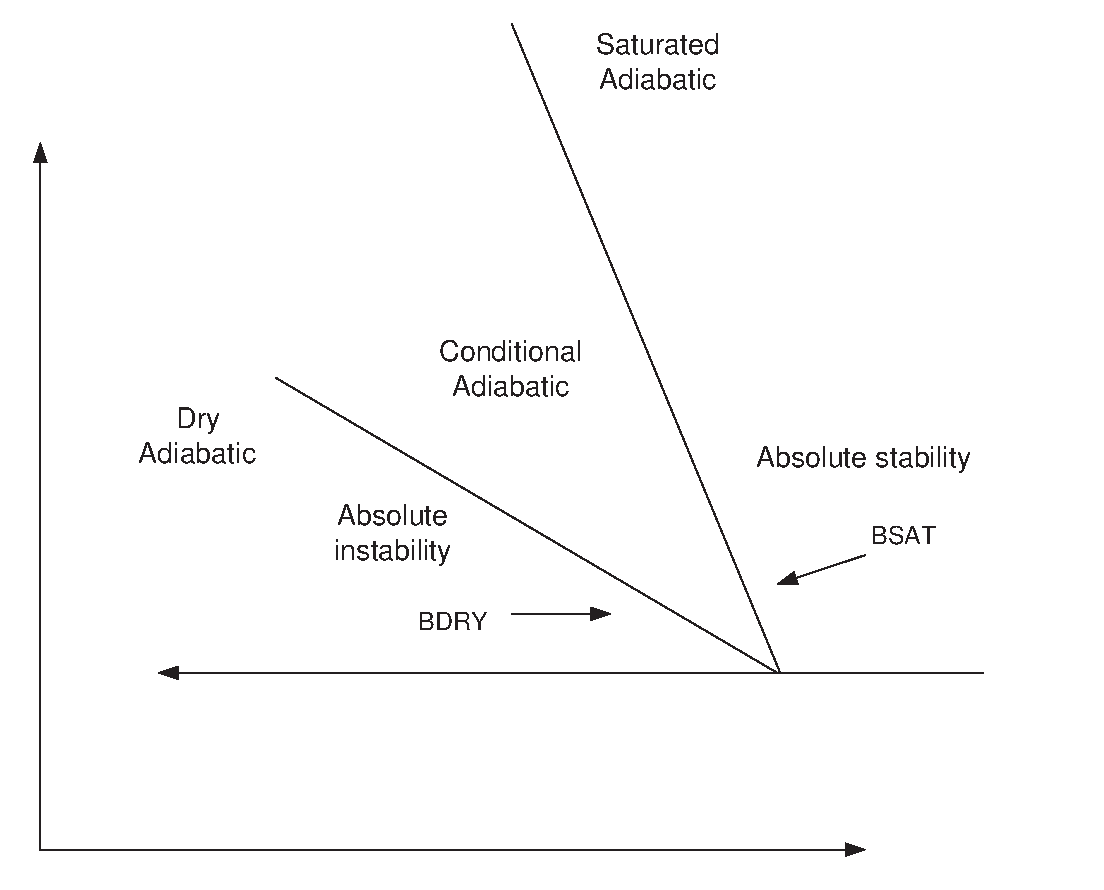
\includegraphics[width=11cm]{vertstab.eps}
    \caption{Stability conditions for the vertical stability of saturated and unsaturated air.} %this is how it shows up in the List of Figures
    \label{f:verticalstab}
    \end{figure}
.\\    
And finally I end this example file with a table which will be centered in the middle of the following page
\begin{table}[hp]
\centering
\renewcommand{\arraystretch}{1.5}
\begin{tabular}{|ll|}
\hline
\multicolumn{2}{|c|}{\bf\sffamily {\it Data} files listed in a table }\\
\hline\hline
\multicolumn{2}{|l|}{\bf\sffamily First part} \\
Fabracadabra.m	& - Saturation computation\\
Fobracadabra.m	& - Pressure computation\\
Fibricadibri.m	& - Permeability computation\\
&\\
\multicolumn{2}{|l|}{\bf\sffamily Structural rock model} \\
struct.m	& - Rock structural data using symmetric boundary condition \\
bstruct.m	& - Rock structural data using anti-symmetric boundary condition \\
\hline
\end{tabular}
\caption{Good-looking program data deck files.} %this is how it shows up in the List of Tables
\label{tbl:tbl}
\end{table}

		
% My part
    %\part{Theory}
    	\include{Chapters/chapter-Introduction}
    	\chapter{Theory} \label{chap:theory}

This chapter describes the theory behind blending and deblending. First the detail hiding operator notation is explained. This notation is used to describe the forward model of seismic data. By introducing the blending operator the forward model is extended to the blended case. Next, the deblending method presented in \citet{Mahdad-Deblending-Method} is discussed to illustrate some of the concepts used in this thesis.

\section{The Forward Model of Blending} \label{sec:Ch-Theory-Operator}
%The detail hiding operator notation was introduced by \citet{Berkhout1982}, and later on it was extended for blended data. 

\subsection{Conventional Seismic Data}
In the detail hiding operator notation \citep{Berkhout1982} the recorded signal is considered discrete in terms of time $t$, receiver position $x_r$, and source position $x_s$. Thus, the measurements can be organized in a cube, $\mathbf{p(t,x_r,x_s)}$ (see Figure \ref{fig:Ch-Theory-DataMatrix}). Each frequency slice of this new cube represents the data matrix, $\mathbf{P}$. 

In the data matrix, $\mathbf{P}$, each column corresponds to a monochromatic common shot gather (see Figure \ref{fig:Ch-Theory-DataMatrixMahdad}), each row to a monochromatic common receiver gather, each diagonal to a monochromatic common offset gather, and each anti-diagonal to a monochromatic common midpoint gather. 

\begin{figure}
    \centering
	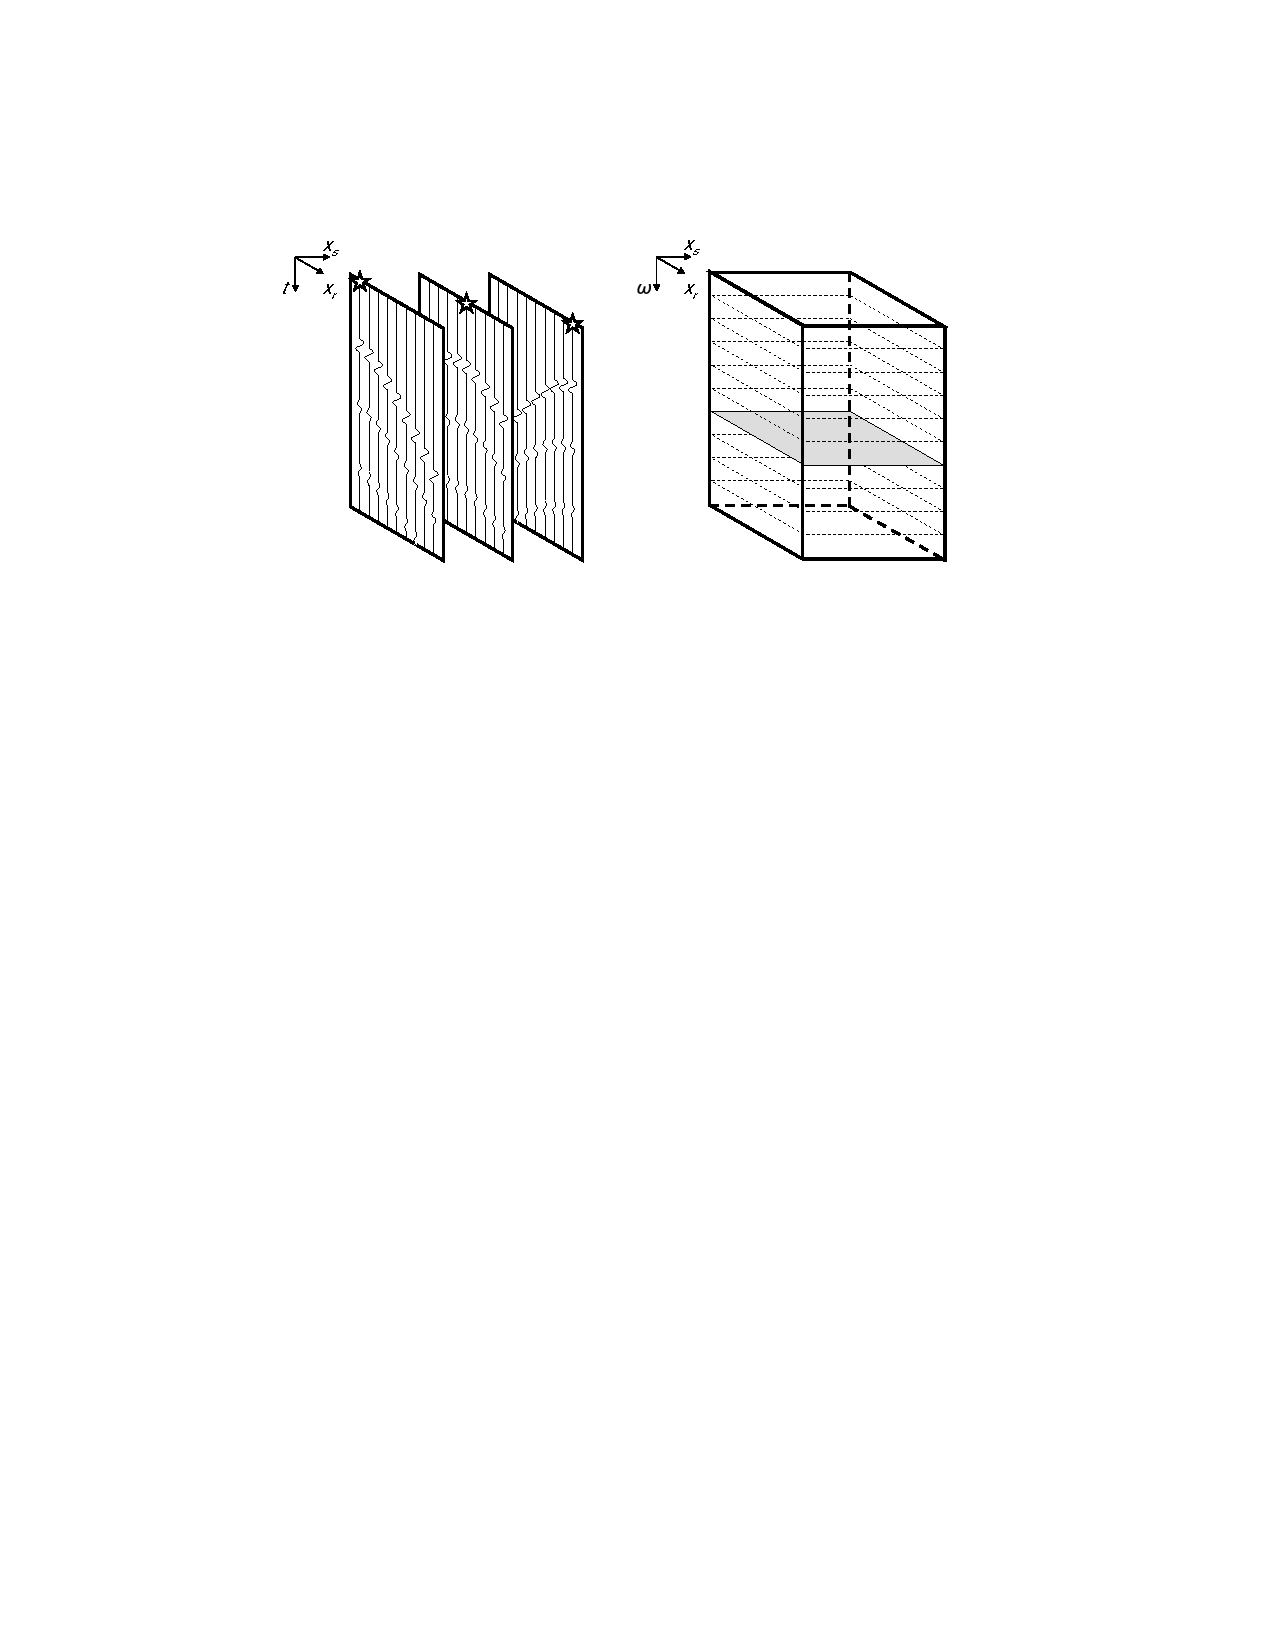
\includegraphics{Plots/P-Groenestijn_2010}
	\caption{Illustration of the data matrix, $\mathbf{P}$, by \citet{Groenestijn_2010}. \textit{Left:} The signal generated at the source position, $x_s$, is measured at receiver position, $x_r$, as a function of time, $t$. Thus, the discretized data is saved in a cube, $\mathbf{p(t,x_r,x_s)}$. \textit{Right:} The cube on the right equals the left cube after a Fourier transform with respect to time. Each frequency slice of the right cube represents the data matrix, $\mathbf{P}$.}
	\label{fig:Ch-Theory-DataMatrix}
\end{figure}


\begin{figure}
    \centering
	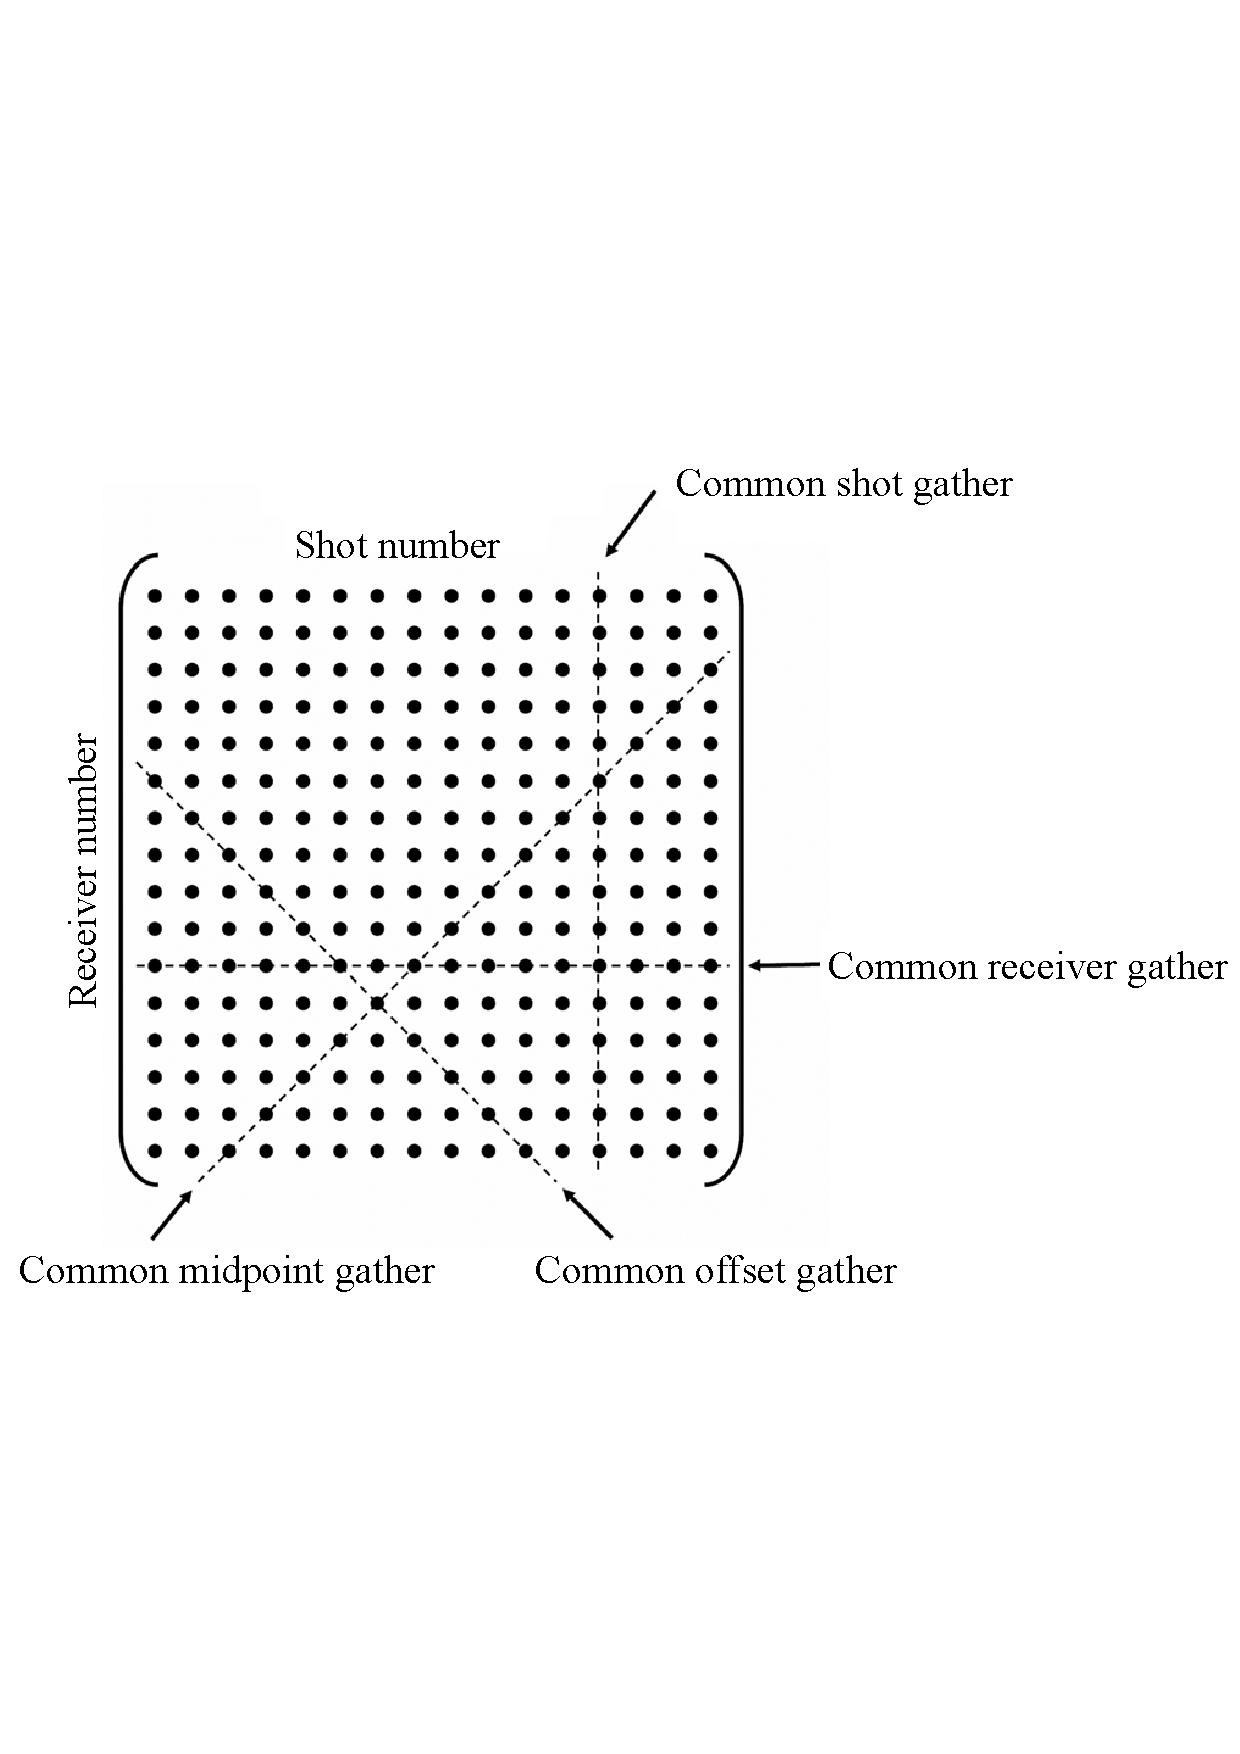
\includegraphics[width = 0.6\textwidth]{Plots/Mahdad-Data-Matrix-edited}
	\caption{Illustration of the data matrix, $\mathbf{P}$, by \cite{Mahdad-Deblending-Method}. The dotted lines indicate directions of common gathers.}
	\label{fig:Ch-Theory-DataMatrixMahdad}
\end{figure}

According to the seismic forward model of \citet{Berkhout1982} the data matrix, $\mathbf{P}$, can be represented by a matrix multiplication of the source matrix, $\mathbf{S}$, the impulse response of the earth, $\mathbf{X}$, and the receiver matrix, $\mathbf{D}$:

\begin{equation}
	\mathbf{P} = \mathbf{D \, X \, S}.
	\label{eq:Ch-Theory-DataRepresentation}
\end{equation}

In the source matrix, $\mathbf{S}$, each row and each column represent one source position (see Figure \ref{fig:Ch-Theory-BlendedSource-Matrices}). Thus, $\mathbf{S}$ is a diagonal matrix. Each diagonal element $s_{ii}$ captures one frequency component of the source signature injected in the earth at the position $x_s = x_i$. By applying a Fourier transform to all frequency components of the element $s_{ii}$ the source signature is obtained.

 The impulse response of the earth, $\mathbf{X}$, describes how an impulse at the source location, $x_s$, is transformed in the earth into the signal at the receiver location, $x_r$.

$\mathbf{D}$ is the receiver matrix, which converts the seismic wavefield at the receiver location $x_r$ to the recorded signal. This includes the forward model of the receiver ghost.

In practice, one tries to retrieve the unknown earth response, $\mathbf{X}$, from the data, $\mathbf{P}$, by removing $\mathbf{S}$ (designature) and $\mathbf{D}$ (receiver deghosting).



\subsection{Blended Seismic Data}

\begin{figure}
	
	\centering
	\begin{subfigure}[t]{0.6\textwidth}	
	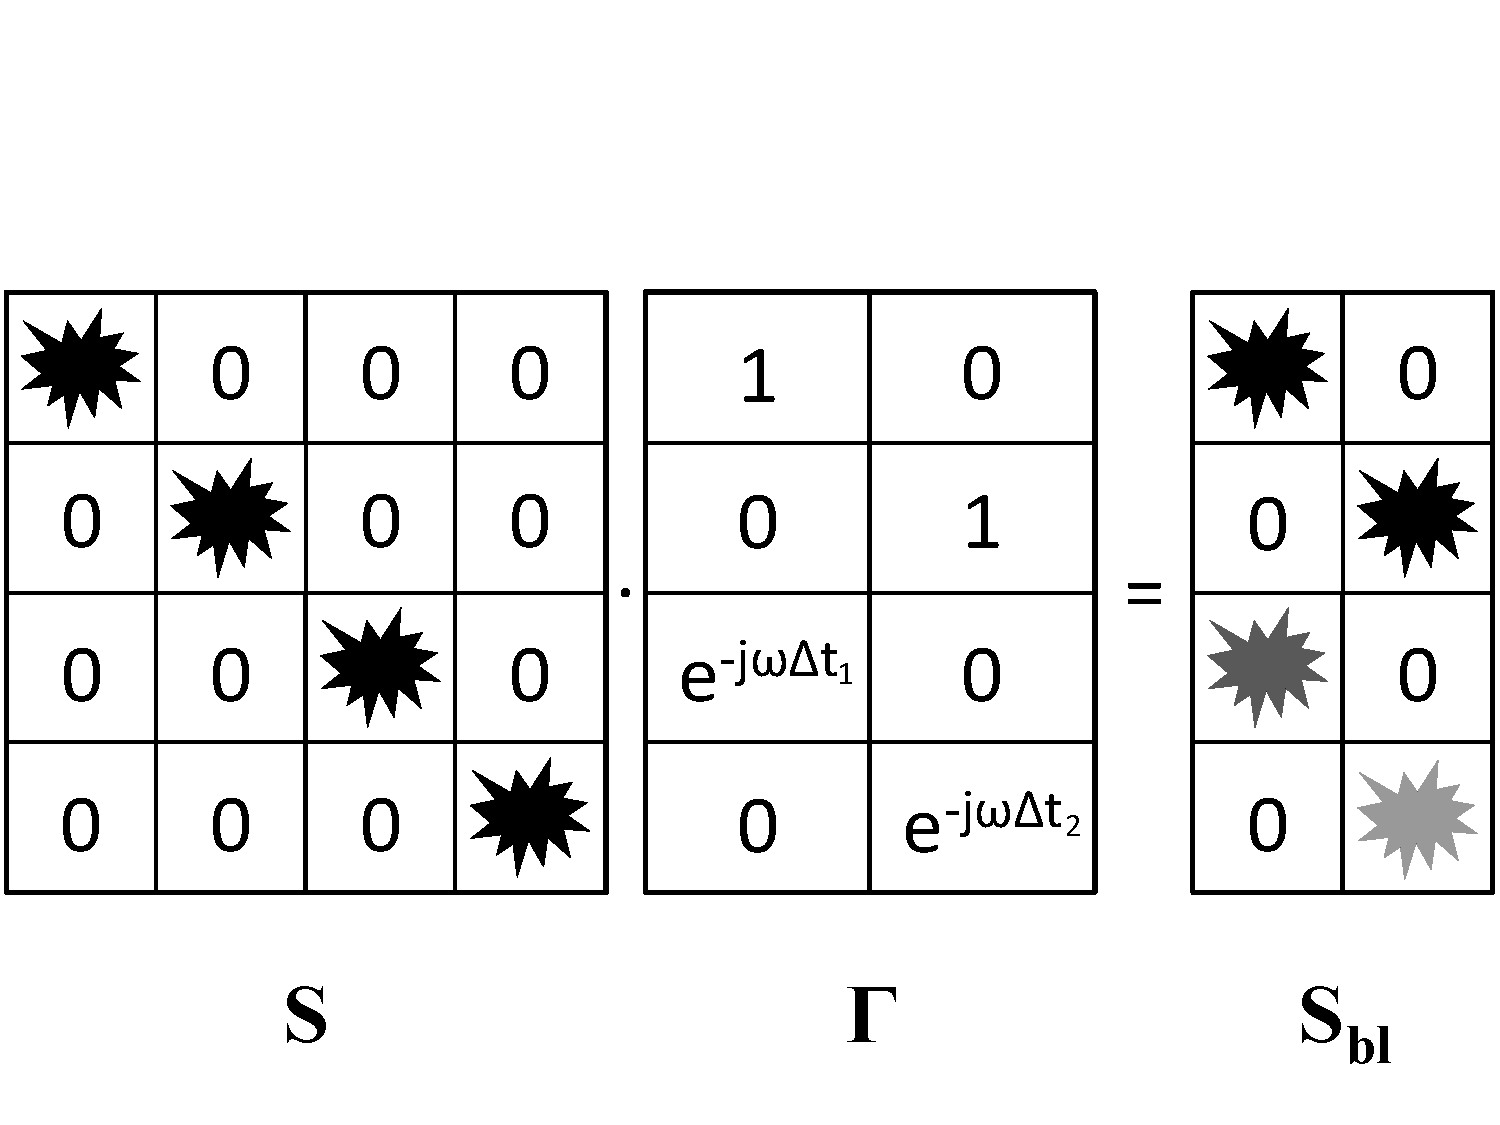
\includegraphics[width=\textwidth]{Plots/Blended-Source-edit2}
	\caption{}
	\label{fig:Ch-Theory-BlendedSource-Matrices}
	\end{subfigure}
	\par\bigskip
	\begin{subfigure}[t]{\textwidth}
	\centering
	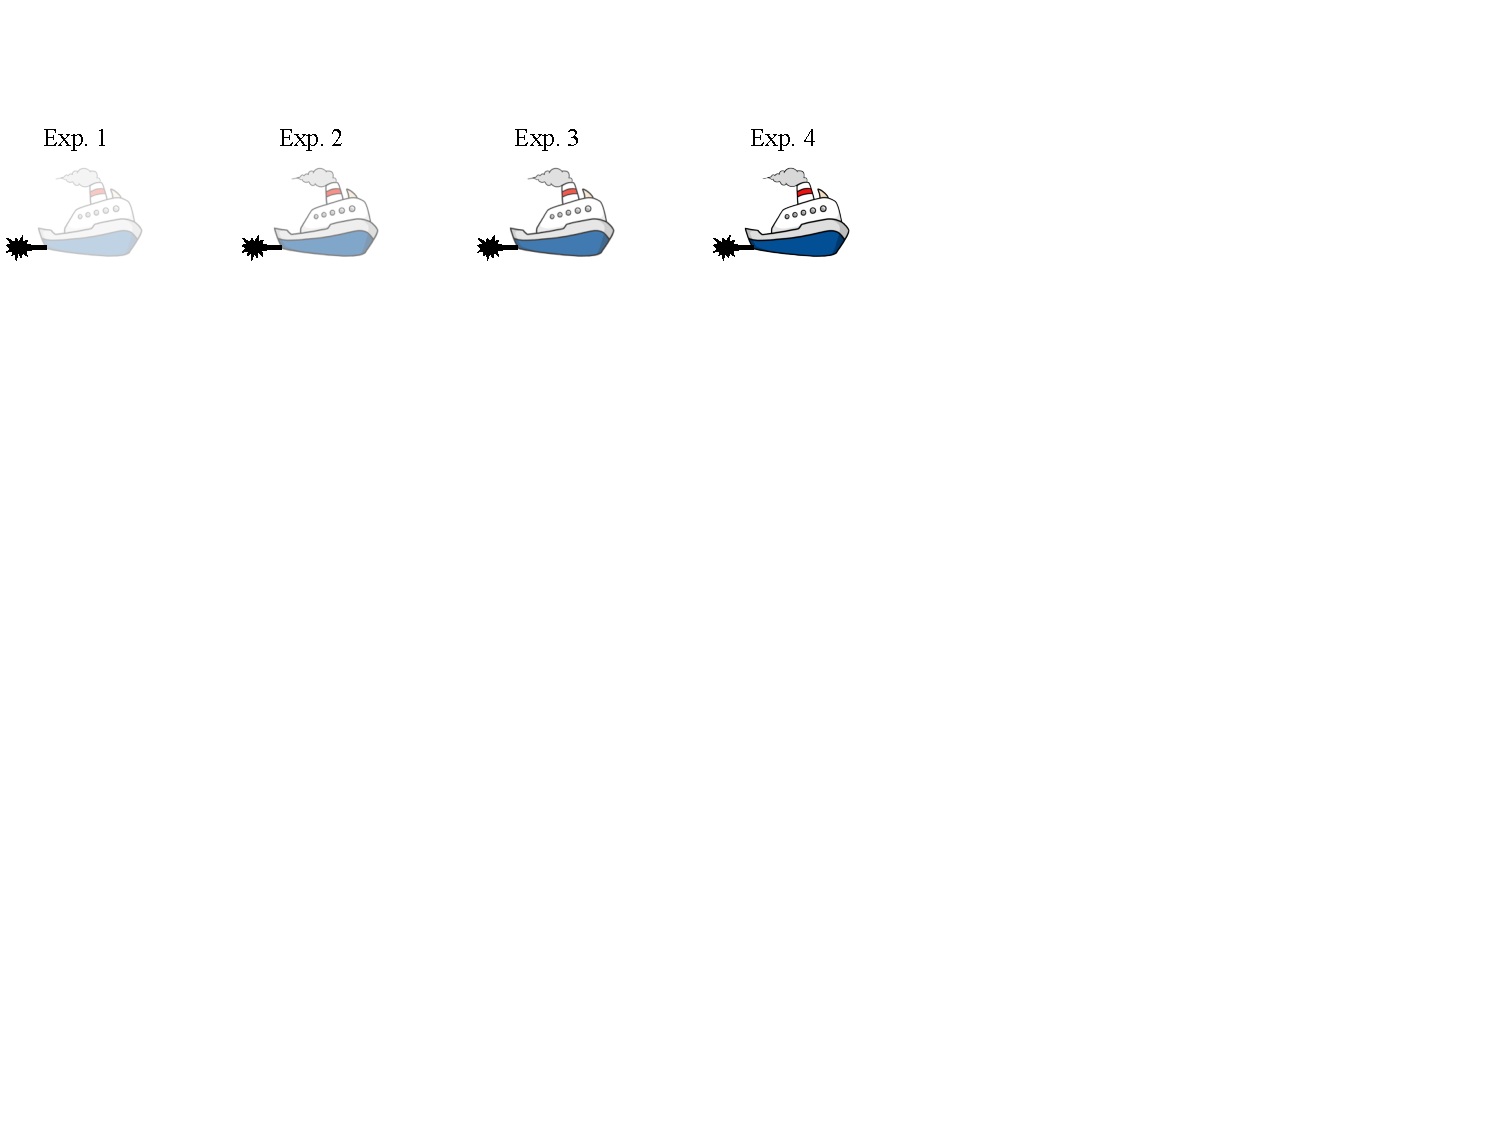
\includegraphics[width=0.5\textwidth]{Plots/Blended-Source-Conventional}
	\caption{}
	\label{fig:Ch-Theory-BlendedSource-Conventional}
	\end{subfigure}
	\par\bigskip
	\begin{subfigure}[t]{\textwidth}
	\centering
	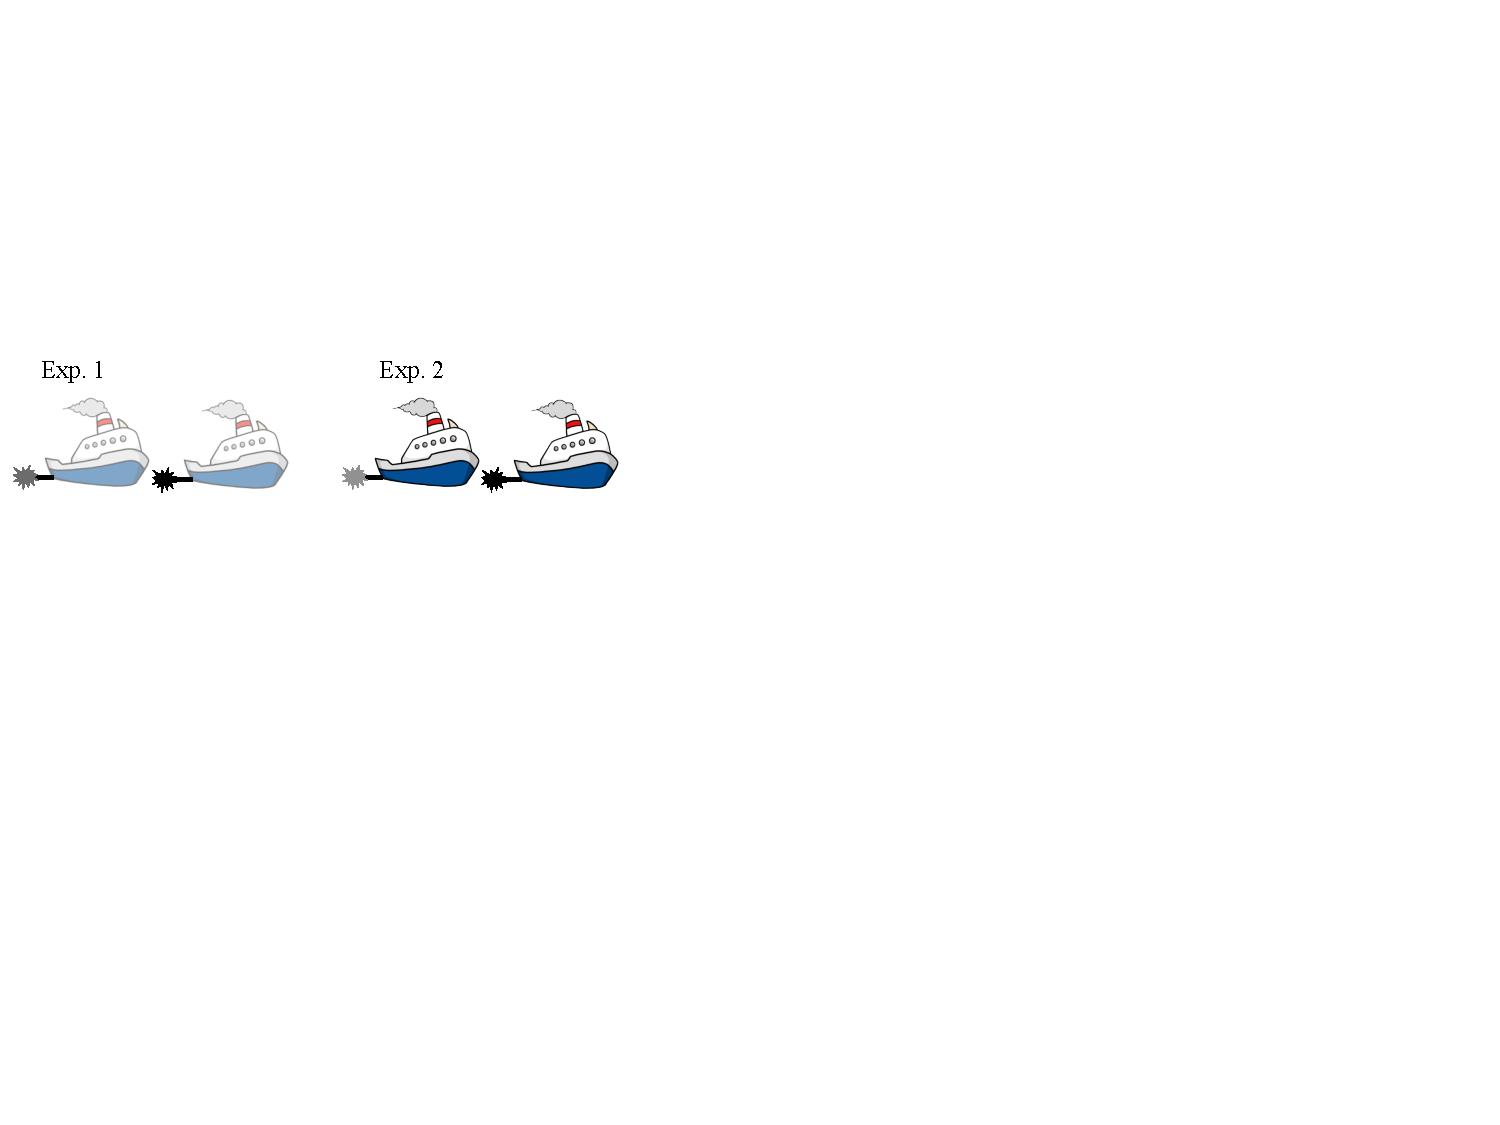
\includegraphics[width=0.36\textwidth]{Plots/Blended-Source-New}
	\caption{}
	\label{fig:Ch-Theory-BlendedSource-Blended}
	\end{subfigure}
    % RATIO of the boat images 294 : 410
	
	\caption{(a) A conventional source matrix, $\mathbf{S}$, is transformed to a blended source matrix, $\mathbf{S}_{bl}$, by applying the blending matrix, $\mathbf{\Gamma}$. Each star represents a source, and the gray scale of the stars represents the relative firing time. (b) Illustration of conventional acquisition with one vessel. This acquisition set up is modeled by the source matrix $\mathbf{S}$. (c) Illustration of blended acquisition with two vessels. In this case the blended source matrix $\mathbf{S}_{bl}$ models the acquisition set up. The experiment number is indicated on top of each drawing.}
	\label{fig:Ch-Theory-BlendedSource}
	
\end{figure}


For blended acquisition the recorded events belonging to different sources overlap as shown in the shot gather in Figure \ref{fig:Ch-Theory-BlendedData}. 

\begin{figure}
	\centering
	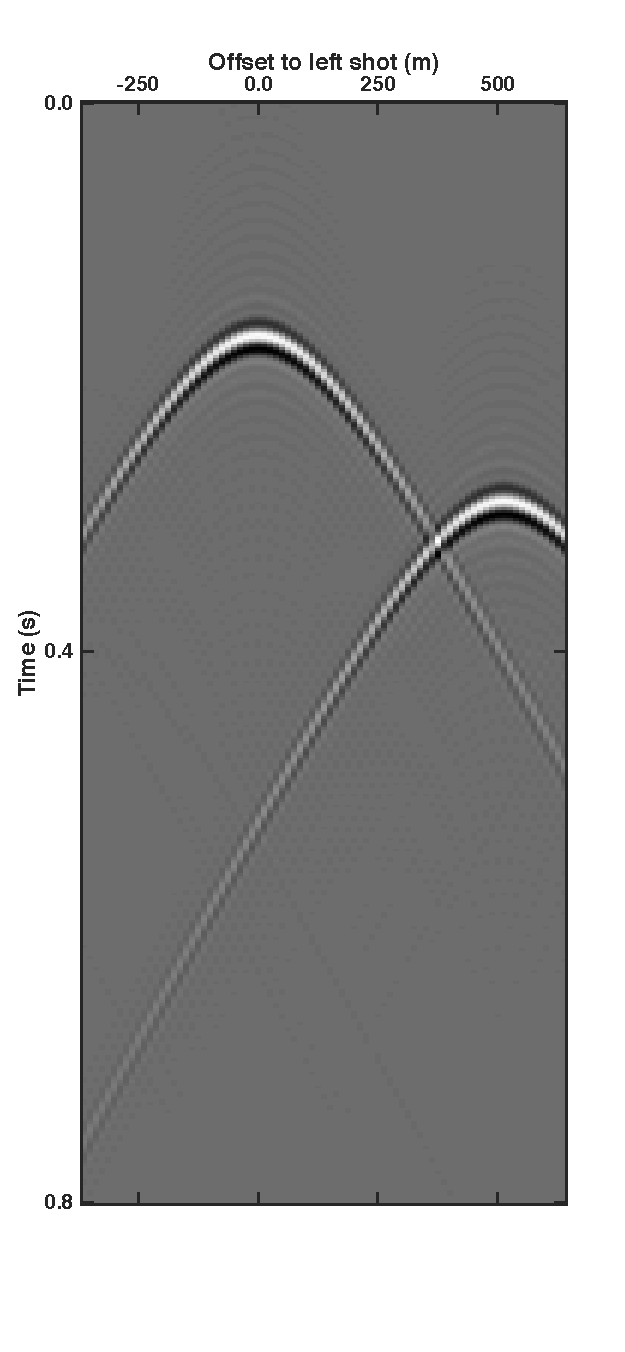
\includegraphics[width=0.25\textwidth]{Plots/Mahdad/30iter/BlendedCSG_sh1-edit_copy}
	\caption{Common shot gather of two blended shots. The shot on the right is fired \SI{120}{\milli\second} after the left shot.}
	\label{fig:Ch-Theory-BlendedData}
\end{figure}

Blending can be captured in the forward model by introducing a blending matrix, $\mathbf{\Gamma}$, which transforms the source matrix, $\mathbf{S}$, into a blended source matrix, $\mathbf{S}_{bl}$,

\begin{equation}
	\mathbf{S}_{bl} = \mathbf{S \, \Gamma}.
	\label{eq:Ch-Theory-BlendedSource}
\end{equation}

 Each row of $\mathbf{\Gamma}$ represents one source, and each column of $\mathbf{\Gamma}$ represents one experiment (see Figure \ref{fig:Ch-Theory-BlendedSource}). 
 
 The blending matrix captures the physics of a blended acquisition as follows: An element $\gamma_{ij}$ of the blending matrix includes a source $i$ and an experiment $j$. If the source $i$ is not fired in the $j^{th}$ experiment the amplitude $A_{ij}$ is zero. If it is fired, source $i$ has a relative amplitude $A_{ij}$ and a relative time delay $t_{ij}$ with respect to the first source fired in the $j^{th}$ experiment;

\begin{equation}
	\gamma_{ij} =  A_{ij} \mathrm{e}^{-j \omega \Delta t_{ij}}.
	\label{eq:Ch-Theory-BlendingElement}
\end{equation}  
 
Thus, the blending matrix selects specific sources from the source matrix and superimposes as visualized in Figure \ref{fig:Ch-Theory-BlendedSource}. From Figure \ref{fig:Ch-Theory-BlendedSource} it also becomes clear that both the blending matrix, $\mathbf{\Gamma}$, and the blended source matrix, $\mathbf{S}_{bl}$, have more rows than columns, i.e. there are more sources than experiments. Thus, the acquisition can be done in less time.

In the case of source blending the receiver matrix, $\mathbf{D}$, is not influenced by blending. And of course, the earth impulse response, $\mathbf{X}$, is independent of the acquisition design. Hence, the blended data can be written as;

\begin{equation}
	\mathbf{P}_{bl} = \mathbf{D} \, \mathbf{X} \, \mathbf{S}_{bl} = \mathbf{D} \, \mathbf{X} \, \mathbf{S} \, \mathbf{\Gamma} = \mathbf{P \, \Gamma}.
	\label{eq:Ch-Theory-BlendedData}
\end{equation}

Note that, the blended data matrix, $\mathbf{P}_{bl}$, also has less columns, i.e. less experiments, than the unblended data matrix, $\mathbf{P}$.



\section{Deblending} \label{sec:MahdadMethod}

Before removing the receiver matrix, $\mathbf{D}$, and the source matrix, $\mathbf{S}$, one must remove  the blending matrix, $\mathbf{\Gamma}$, from the blended data, $\mathbf{P}_{bl}$. This process is called deblending.

The deblending method presented in this thesis builds on the method of \citet{Mahdad-Deblending-Method}. Therefore, the method of \citet{Mahdad-Deblending-Method} is described in great detail.

The basic workflow of the method of \citet{Mahdad-Deblending-Method} is summarized in Figure \ref{fig:Ch-Theory-FlowChart} and will be explained step by step in the following subsections. 

\begin{figure}
	\centering
	\includegraphics[width=0.8\textwidth]{Plots/Mahdad-FlowChart-v5}
	\caption{Flowchart belonging to the deblending method of \citet{Mahdad-Deblending-Method}.}
	\label{fig:Ch-Theory-FlowChart}
\end{figure}

\subsection{Pseudo-Deblending}

Unfortunately, the inverse problem of equation \ref{eq:Ch-Theory-BlendedData} is underdetermined, which means that there is not a unique solution for the unblended data, $\mathbf{P}$. Thus, additional constraints are required to deblend the data, which are (1) sparsity of the signal in the $x$-$t$-domain and (2) coherency of the signal in the $f$-$k$-domain. 

The first estimate of the unblended data matrix, $\mathbf{P}$, is obtained by pseudo-deblending;

\begin{equation}
	\mathbf{P}_{ps} = \mathbf{P}_{bl} \, \mathbf{\Gamma}^H.
	\label{eq:Ch-Theory-PseudoDeblended}
\end{equation}

Pseudo-deblending copies the blended data to the locations of all shots present in the blended shot and shifts them  upward in time to compensate for the time delay. For example, Figure \ref{fig:Ch-Theory-PseudoDeblendedCSG2} and \ref{fig:Ch-Theory-PseudoDeblendedCSG} shows the two pseudo-deblended shot gathers of the blended data in Figure \ref{fig:Ch-Theory-BlendedData}. Note that the pseudo-deblended data have the same size as $\mathbf{P}$.


\subsection{Common Receiver Gather}
By transforming the data to another domain, e.g. to the common receiver domain, the interfering sources become incoherent and are visible as spiky noise (see Figure \ref{fig:Ch-Theory-PseudoDeblendedCRG}). Therefore, the interfering sources can be attenuated with a noise filter. 

%\todo[inline]{MOVE TO EXTENSION PART: Considering the 1/b factor, the interfering source creates blending noise and scales the amplitude of the shot of interest. So, is it correct to set blending noise and interfering source equal?}

\begin{figure}
	\centering
	\begin{subfigure}[t]{0.25\textwidth}
		\centering
		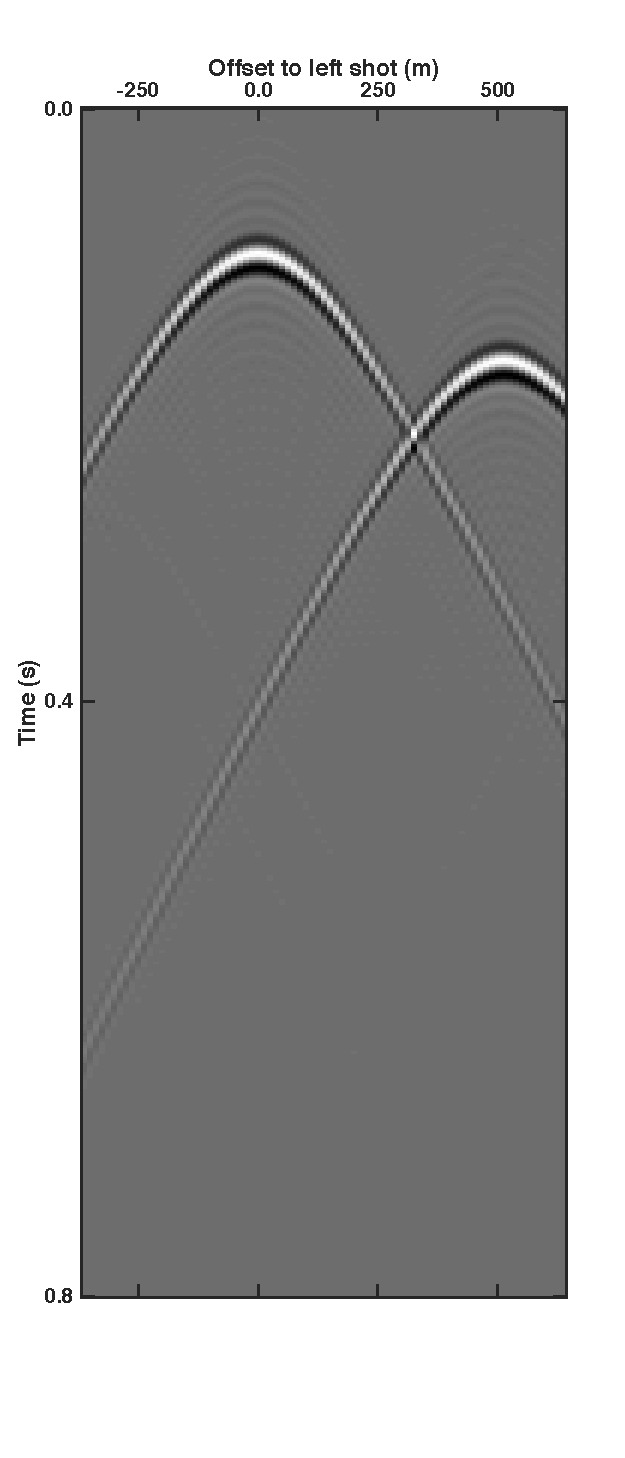
\includegraphics[width=0.925\textwidth]{Plots/Mahdad/30iter/Pseudo-DeblendedCSG_sh2}	
		\caption{Common-shot-gather}
		\label{fig:Ch-Theory-PseudoDeblendedCSG2}
	\end{subfigure}
	%
	\centering
	\begin{subfigure}[t]{0.25\textwidth}
		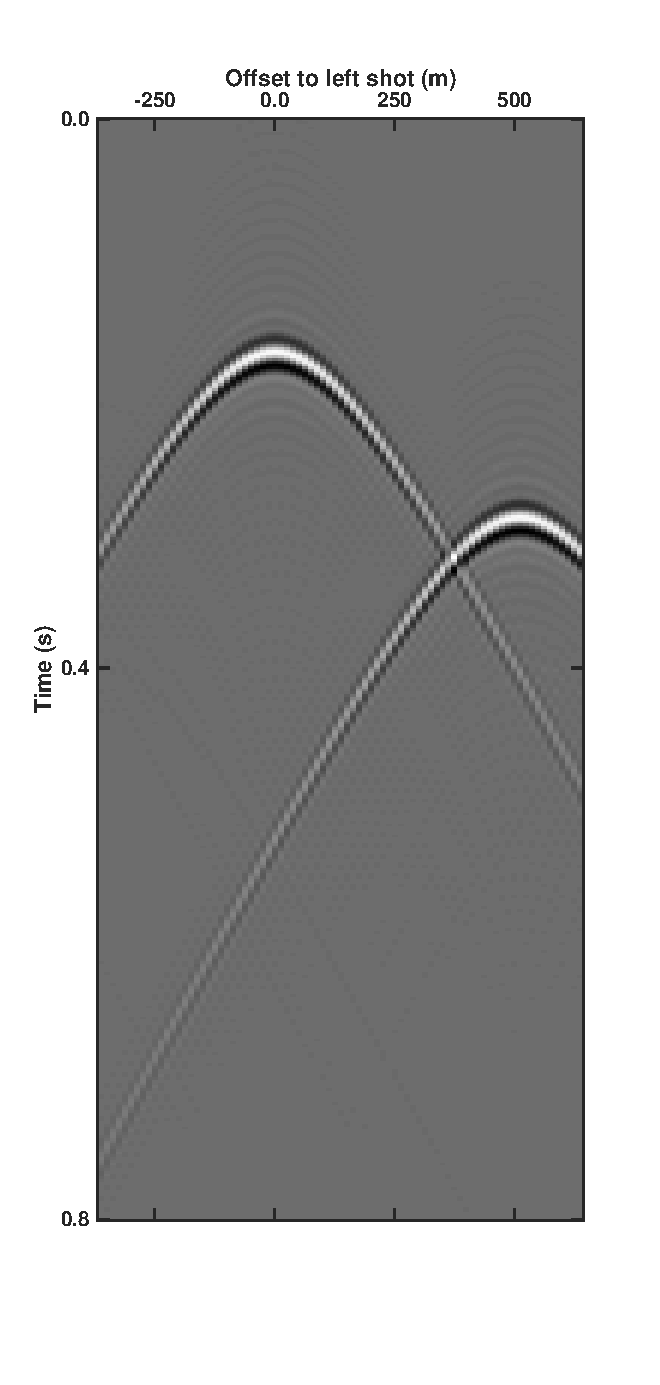
\includegraphics[width=\textwidth]{Plots/Mahdad/30iter/Pseudo-DeblendedCSG_sh1}	
		\caption{Common-shot-gather}
		\label{fig:Ch-Theory-PseudoDeblendedCSG}
	\end{subfigure}
	%
	\centering
	\begin{subfigure}[t]{0.25\textwidth}
		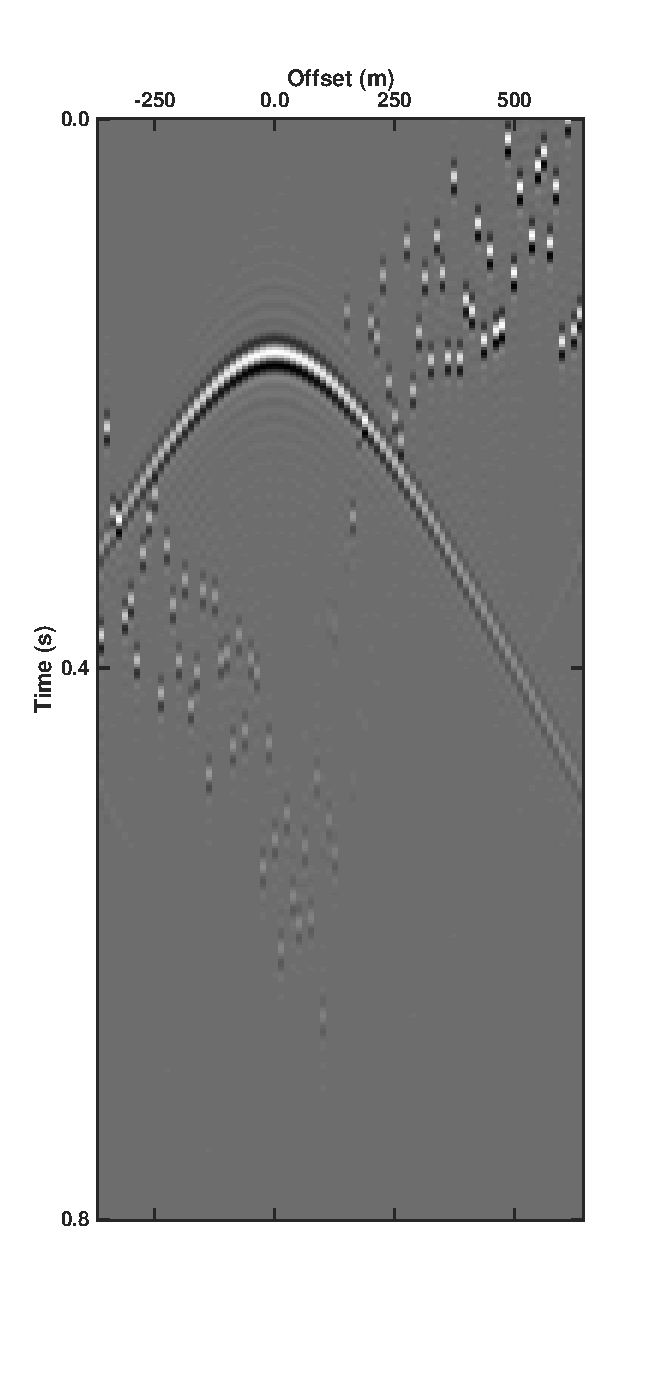
\includegraphics[width=\textwidth]{Plots/Mahdad/30iter/Pseudo-DeblendedCRG_rec30}	
		\caption{Common-receiver-gather}
		\label{fig:Ch-Theory-PseudoDeblendedCRG}
	\end{subfigure}
	\caption{Pseudo-deblended data, $\mathbf{P}_{ps}$, sorted in common shot gathers (a,b) and in a common receiver gather (c). The pseudo-deblended data of the right shot (a) and the left shot (b,c) were shifted by different time delays. The overlapping sources map in the pseudo-deblended shot gathers as coherent events, while they map as incoherent spikes in the pseudo-deblended receiver gather.}
	\label{fig:Ch-Theory-PseudoDeblended}

\end{figure}


\subsection{Iterative Blending Noise Estimation} \label{sec:IterBlenNoiseEst}

In an ideal case the noise generated by the interfering sources, the so called blending noise, is calculated with the unblended data,

\begin{equation}
	\mathbf{N} = \mathbf{P}_{bl} \, \mathbf{\Gamma}^H - \mathbf{P} = \mathbf{P}_{ps} - \mathbf{P}.
	\label{eq:Ch-Theory-Noise}
\end{equation}

Obviously, in practice the unblended data is unknown and must be estimated by adding extra constraints. The loop shown in Figure \ref{fig:Ch-Theory-FlowChart} applies the constraints to reduce the blending noise iteratively until the solution is obtained. 

In the following all the quantities which are estimated are indicated with a hat. The steps of the iterative blending noise estimation are demonstrated in Figure \ref{fig:Ch-Theory-IterativeDeblending}.

\begin{figure}
	\centering
	\begin{subfigure}[t]{0.25\textwidth}
		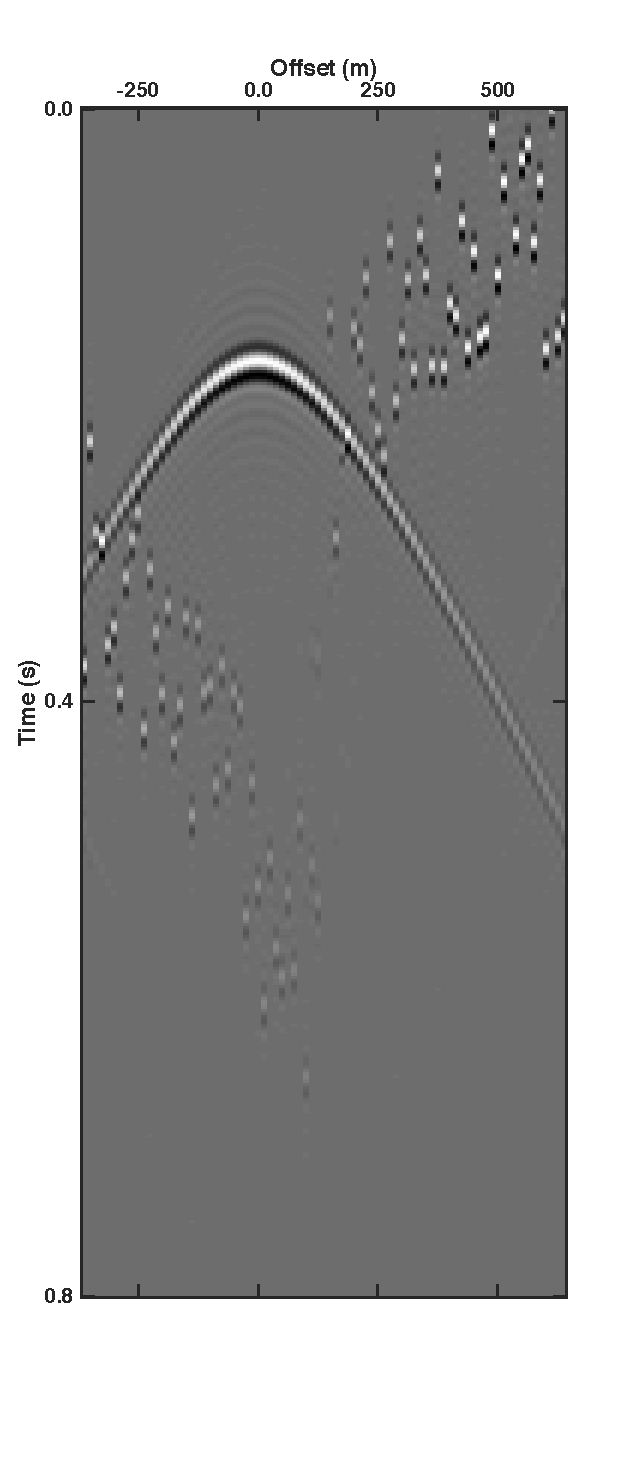
\includegraphics[width=\textwidth]{Plots/Mahdad/5iter/Pseudo-DeblendedCRG_rec30}	
		\caption{}
		\label{fig:Ch-Theory-PseudoDeblendedCRG5}
	\end{subfigure}
	%
	\centering
	\begin{subfigure}[t]{0.25\textwidth}
		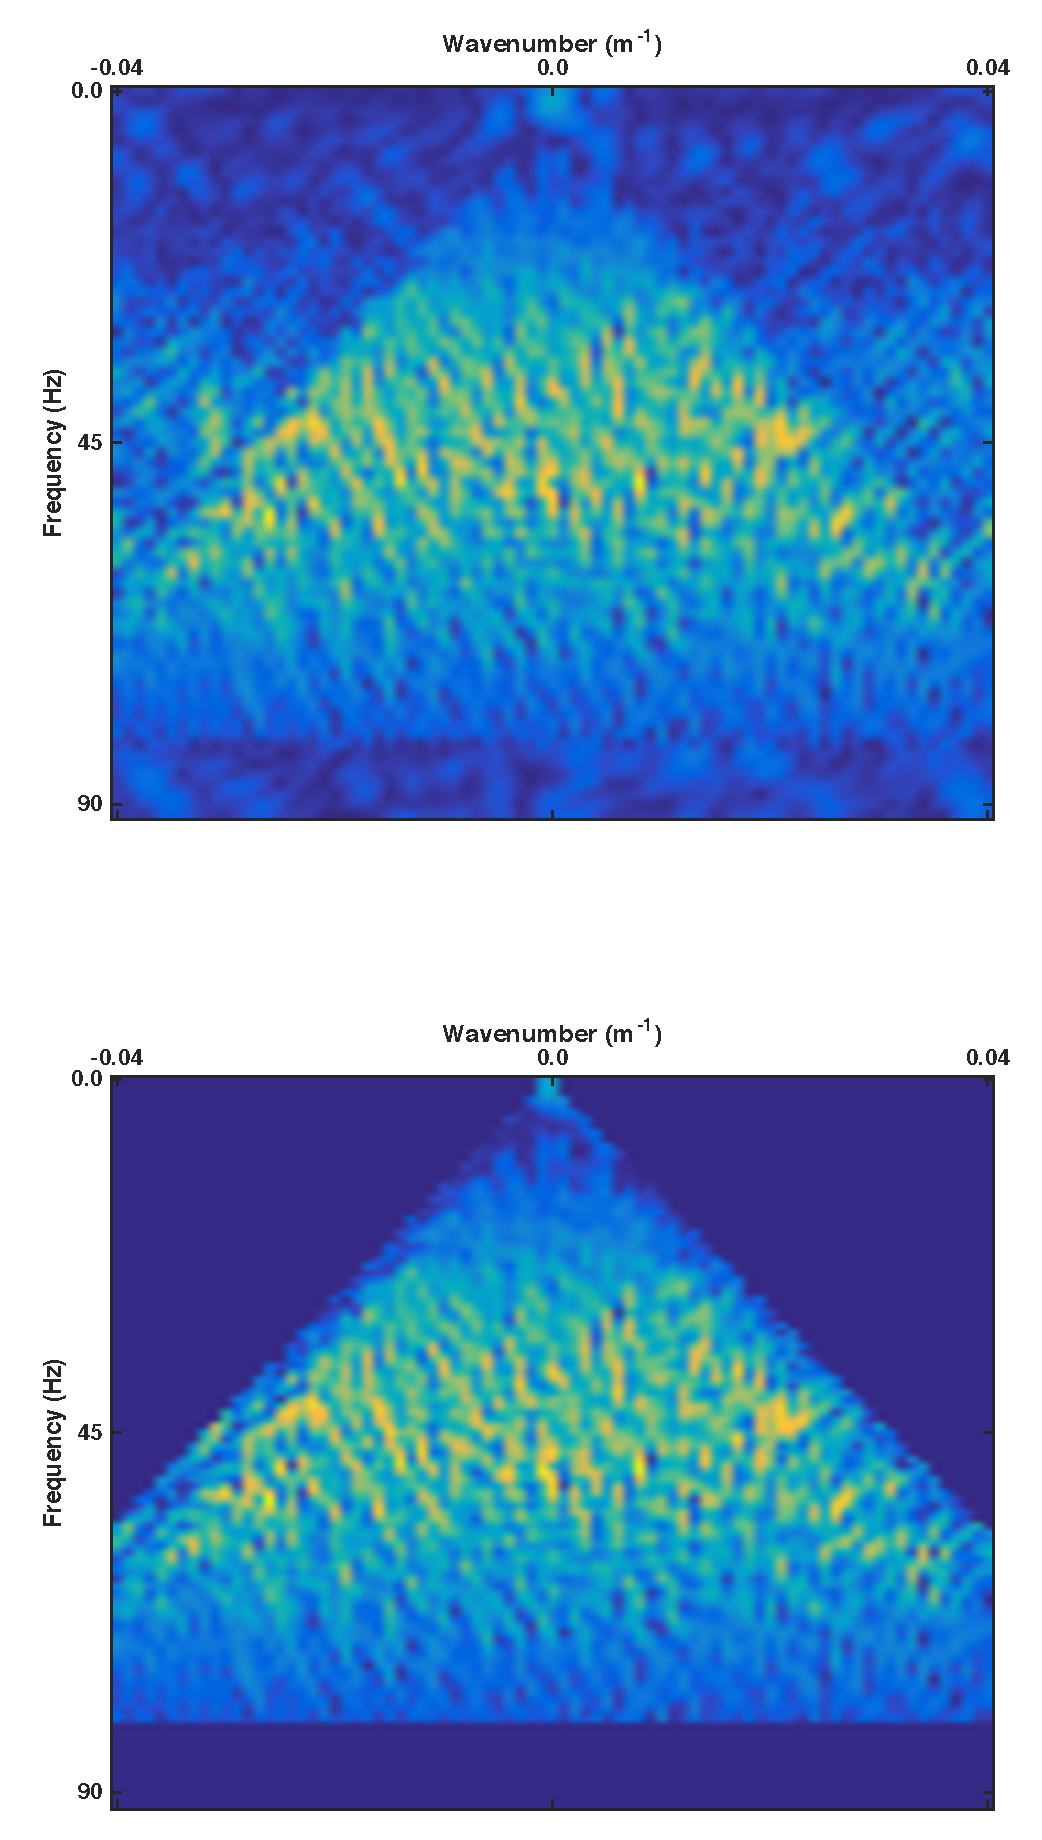
\includegraphics[width=\textwidth]{Plots/Mahdad/5iter/FK-Spectra}	
		\caption{}
		\label{fig:Ch-Theory-FKDeblended-NoFilter}
	\end{subfigure}
	%
	\begin{subfigure}[t]{0.25\textwidth}
		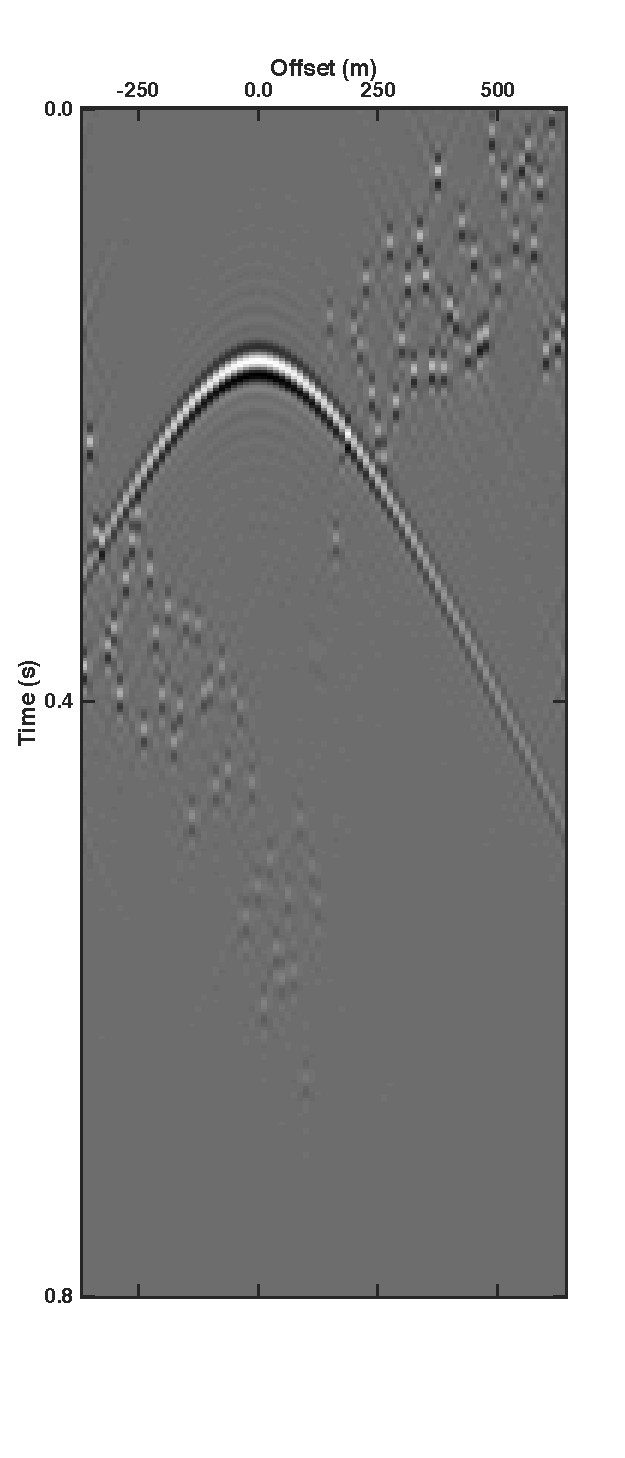
\includegraphics[width=\textwidth]{Plots/Mahdad/5iter/FkFilteredCRG_rec30}	
		\caption{}
		\label{fig:Ch-Theory-FKFiltered}
	\end{subfigure}
	%
	\begin{subfigure}[t]{0.25\textwidth}
		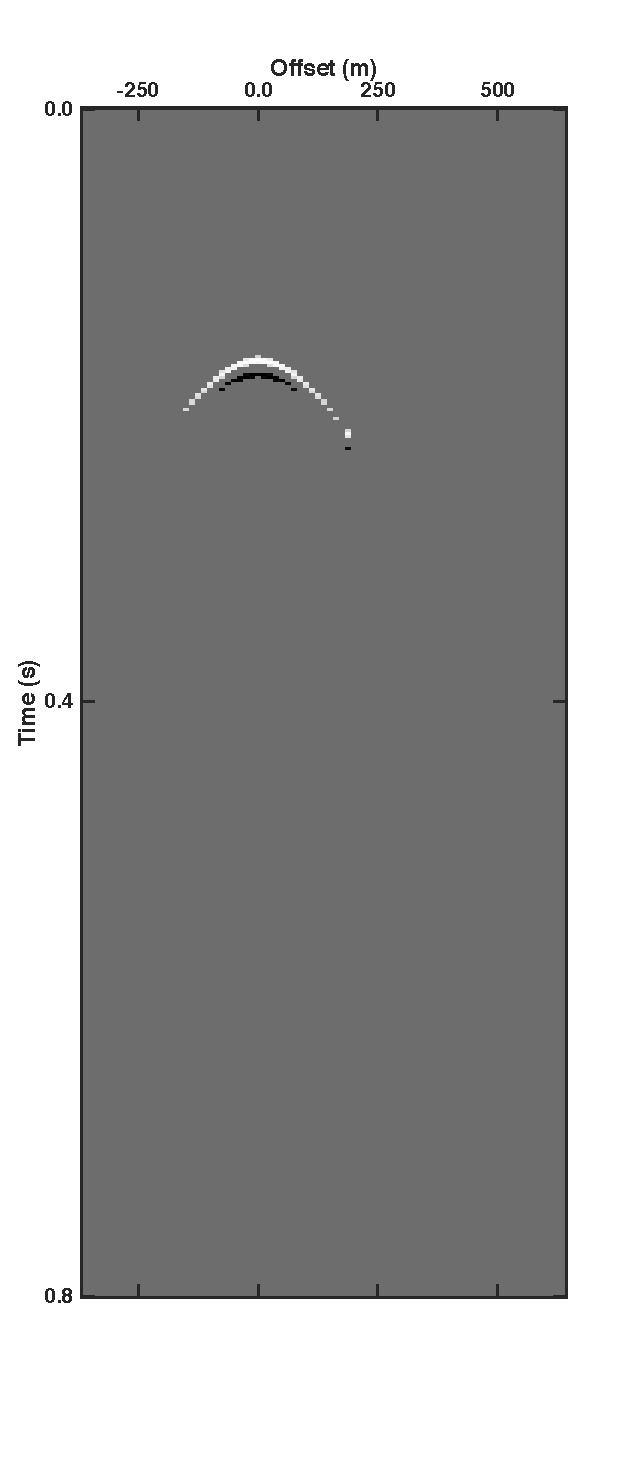
\includegraphics[width=\textwidth]{Plots/Mahdad/5iter/ThresholdCRG_rec30}	
		\caption{}
		\label{fig:Ch-Theory-Threshold}
	\end{subfigure}
	%
	\begin{subfigure}[t]{0.25\textwidth}
		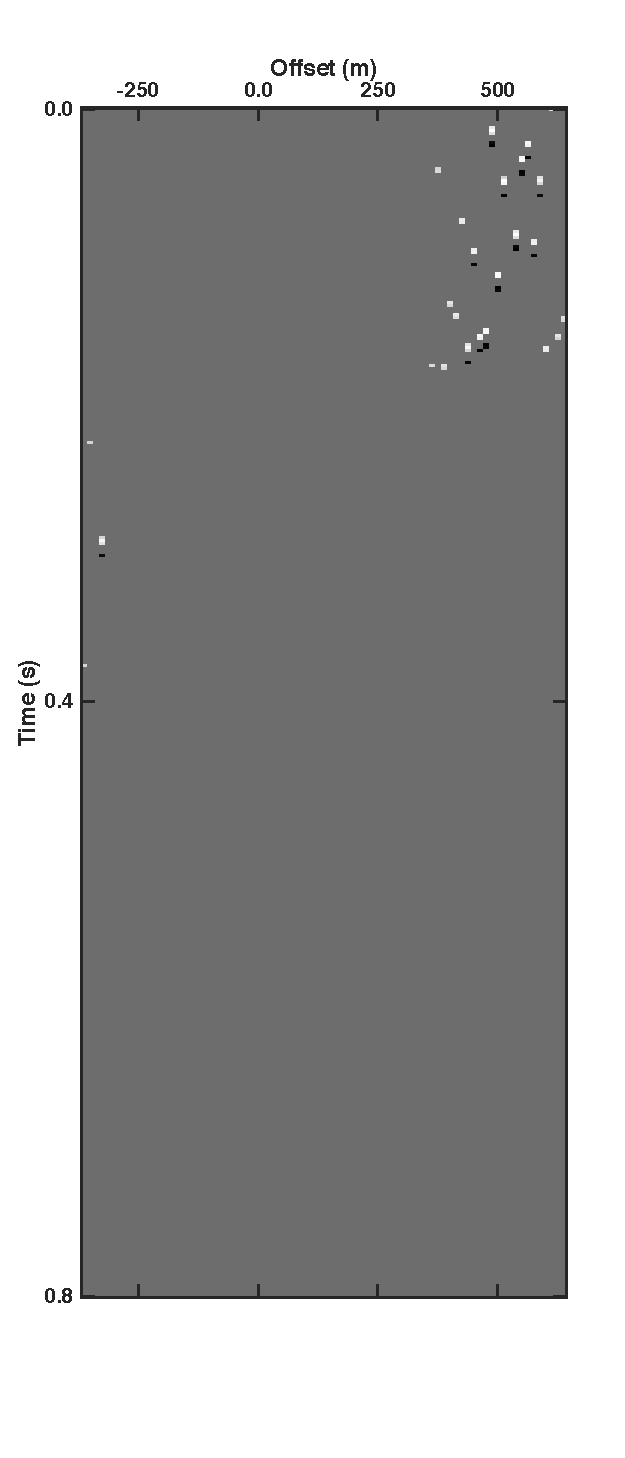
\includegraphics[width=\textwidth]{Plots/Mahdad/5iter/NoiseCRG_rec30}	
		\caption{}
		\label{fig:Ch-Theory-Noise}
	\end{subfigure}
	%
	\begin{subfigure}[t]{0.25\textwidth}
		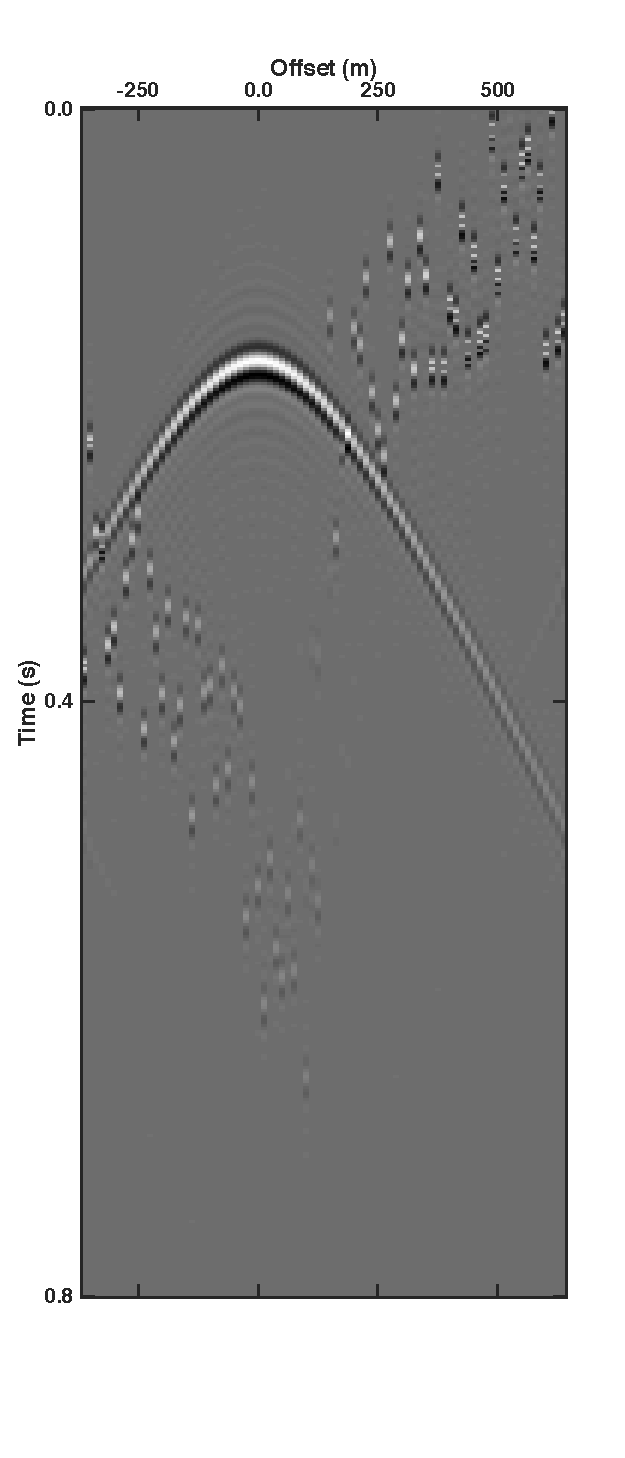
\includegraphics[width=\textwidth]{Plots/Mahdad/5iter/DeblendedCRG_rec30}	
		\caption{}
		\label{fig:Ch-Theory-Deblended}
	\end{subfigure}
	\caption{(a) Pseudo-deblended receiver gather. The subfigures (b)-(f) illustrate each step of the deblending algorithm. For better visibility examples from the $5^{th}$ iteration are chosen. (b) $f$-$k$-spectrum before (top) and after (bottom) $f$-$k$-filtering, (c) $f$-$k$-filtered common receiver gather, (d) after thresholding, (e) estimated source interference (f) estimated data.}
	\label{fig:Ch-Theory-IterativeDeblending}
\end{figure}


\subsubsection*{F-K-Filtering}

One of the constraints is coherency, i.e. by assuming the blending noise in Figure \ref{fig:Ch-Theory-PseudoDeblendedCRG} is incoherent it can be removed. For this purpose the data is transformed from the space time to the wavenumber frequency domain where the spiky noise spreads over all wavenumber and frequency components (see Figure \ref{fig:Ch-Theory-FKDeblended-NoFilter}, top). 

%For a 2D $f$-$k$-spectrum the minimum (physical) velocity of the subsurface, $v_{min}$, determines the maximum wavenumber, $k_{max}$,  for a given frequency, $f$;

The unblended data maps in the $f$-$k$-domain as a cone (see Figure \ref{fig:Ch-Theory-fk-Unblended-data}). The minimum (physical) velocity, $v_{min}$, of the subsurface determines the slope of the cone. This means that for a given frequency, $f$, the maximum wavenumber, $k_{max}$, is defined as; 

\begin{equation}
	k_{max} = \frac{f}{v_{min}}.
	\label{eq_Ch-Theory-MaxWavenmber}
\end{equation} 

In the marine case the minimum velocity is usually the water velocity, $v_{w} = \SI{1500}{\metre\per\second}$.

\begin{figure}
	\centering
	\begin{subfigure}[t]{0.45\textwidth}
		\centering
		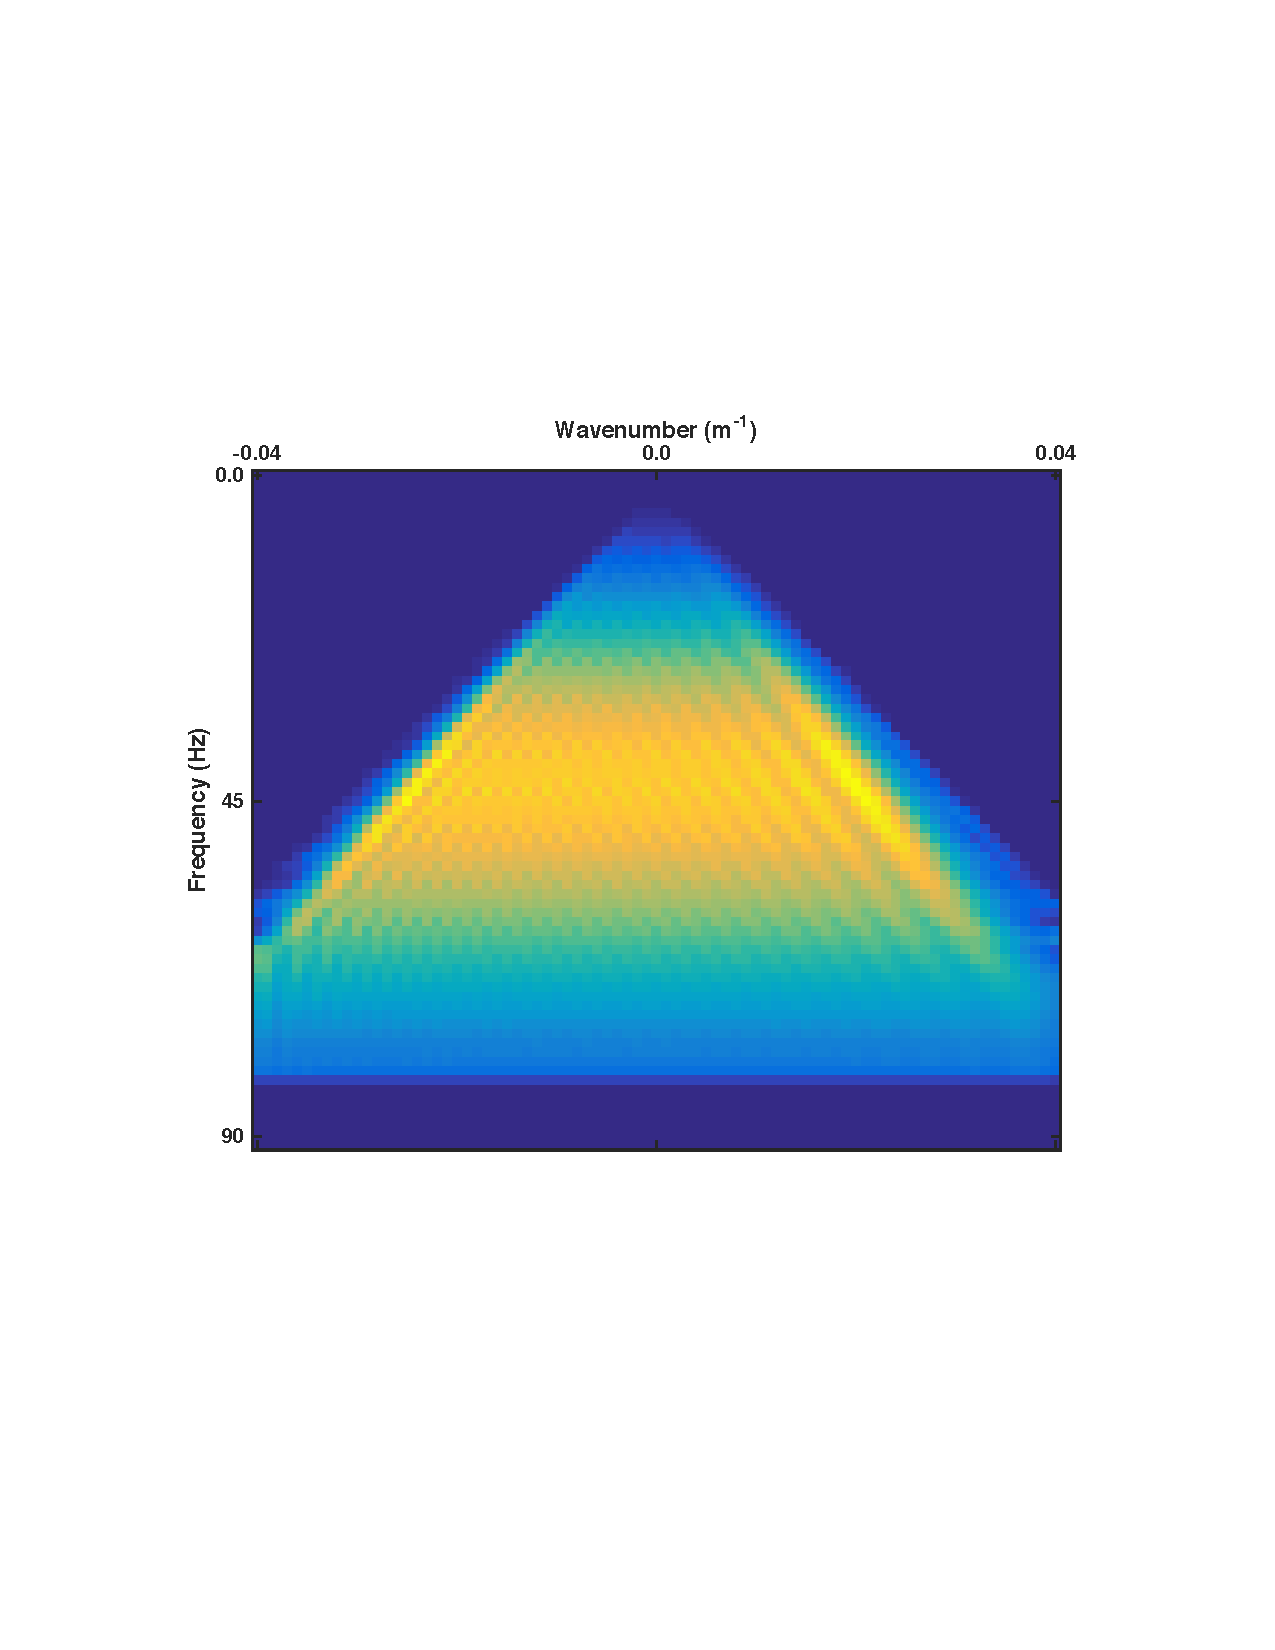
\includegraphics[width = \textwidth]{Plots/Mahdad/30iter/FK-UnblendedCRG_r1}
		\caption{$f$-$k$-spectrum of an unblended common shot gather.}
		\label{fig:Ch-Theory-fk-Unblended-data}
	\end{subfigure}
	%
	\centering
	\begin{subfigure}[t]{0.45\textwidth}
		\centering
		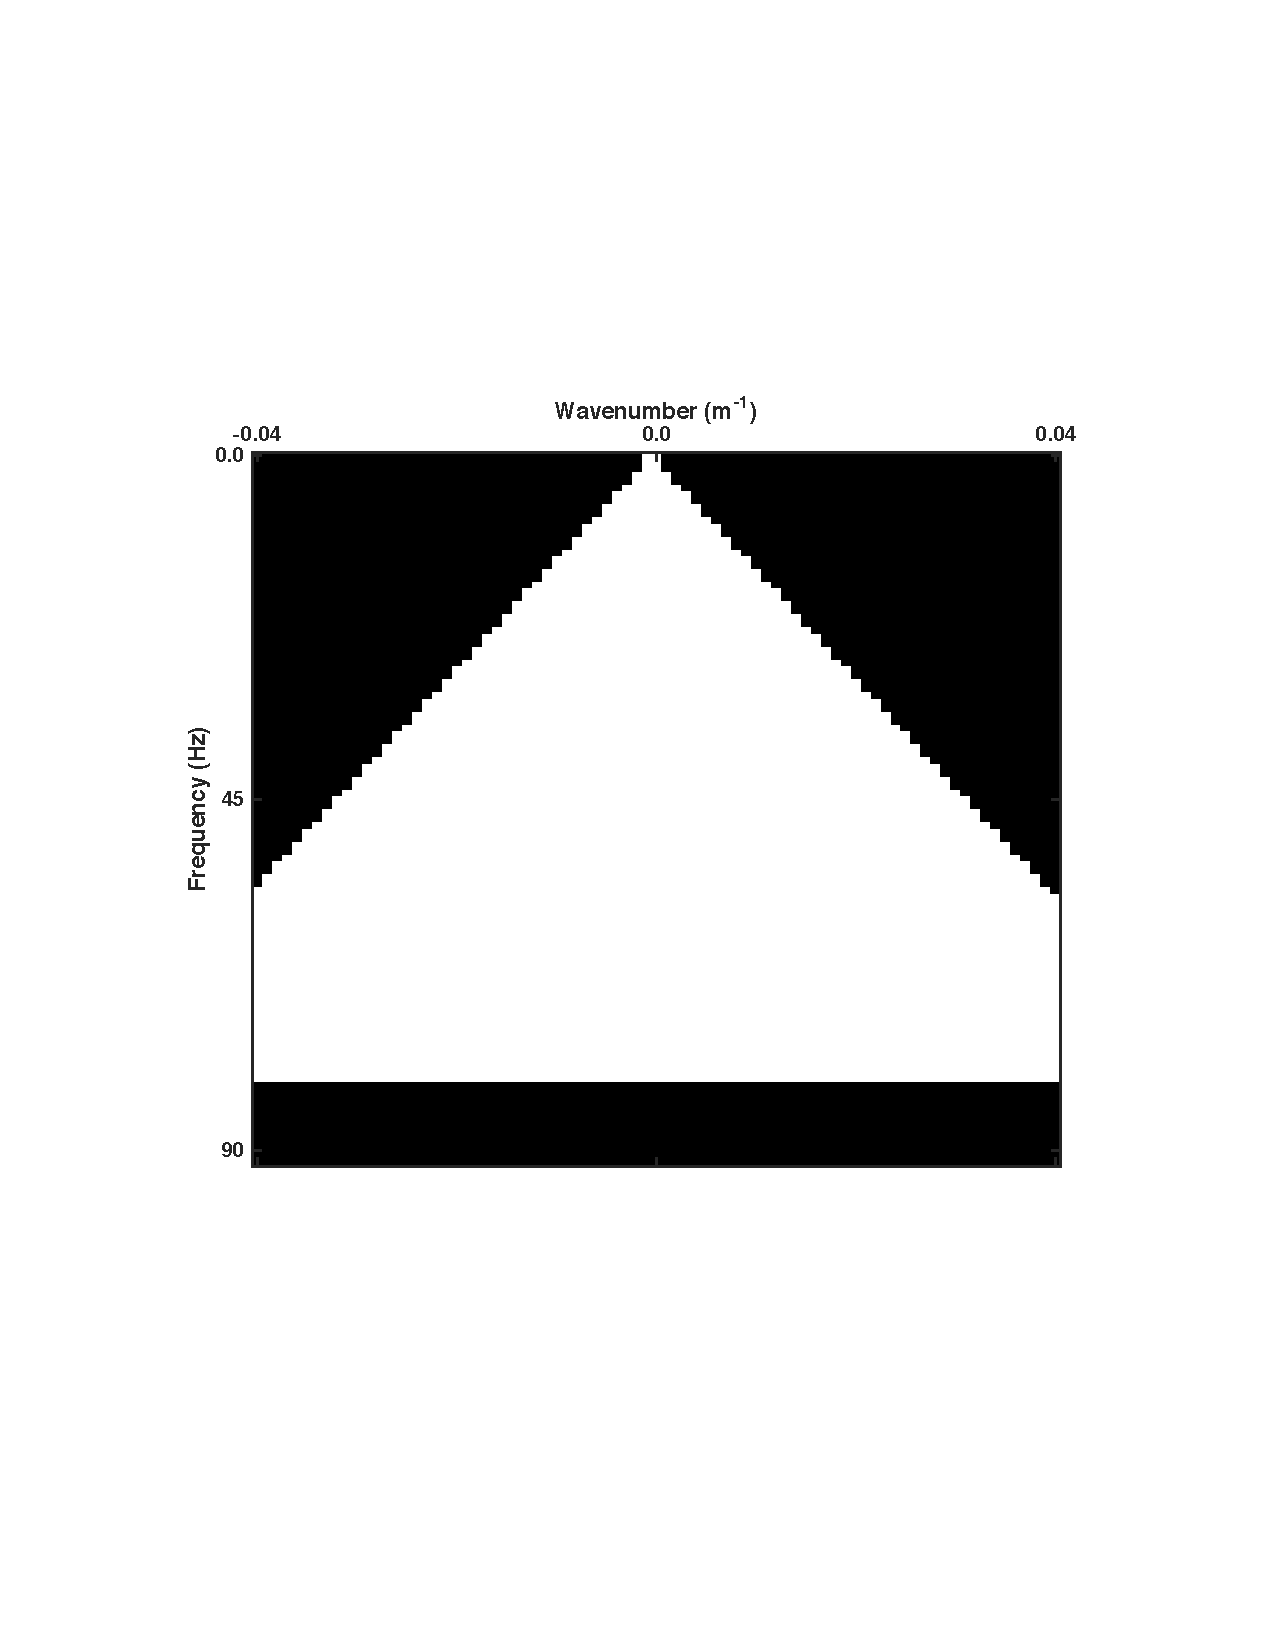
\includegraphics[width = 0.957\textwidth]{Plots/Mahdad/5iter/FK-MaskCRG_rec30}
		\caption{The $f$-$k$-mask is determined by the minimum signal velocity in the subsurface. The white area of the filter equals one, the black area equals zero. Thus, the filter removes data which is mapped outside of the white signal cone.}
		\label{fig:Ch-Theory-FK-Mask}
	\end{subfigure}
	
	\caption{}
	\label{fig:Ch-Theory-fk-unblended-data-mask}
\end{figure}

For each frequency, $f$, wavenumbers above $k_{max}$ are removed which results in a 2D $f$-$k$-filter as depicted in Figure \ref{fig:Ch-Theory-FK-Mask}.

The $f$-$k$-filter removes the part of the blending noise, which maps outside of the signal cone. Thus, after transforming the data back to the space time domain the amplitudes of the spiky noise are attenuated (see Figure \ref{fig:Ch-Theory-FKFiltered}). 

Note that $f$-$k$-filtering can only reduce unaliased frequency components of the blending noise. In Figure \ref{fig:Ch-Theory-FK-Mask} the highest unaliased frequency is defined by the point where the white cone intersects with the frequency axis, i.e. at \SI{60}{\hertz}. 

The high cut frequency of the $f$-$k$-mask is set according to the highest frequency components in the data. The aliased blending noise will pass the $f$-$k$-filter and will be reduced afterwards by thresholding. 


\subsubsection*{Thresholding}

The second constraint for the estimation of the unblended data is sparsity of the signal in the space time domain.

After $f$-$k$-filtering the spiky noise is attenuated (see Figure \ref{fig:Ch-Theory-FKFiltered}). Consequently, the signal amplitudes are now stronger than the noise amplitudes. This allows to define a threshold in the $x$-$t$ domain, which is larger than the noise amplitudes and smaller than the highest signal amplitudes. Only amplitudes above the threshold are picked, i.e. only signal with strong amplitudes is selected (see Figure \ref{fig:Ch-Theory-Threshold}). 

\subsubsection*{Interference Estimation}

The resulting thresholded data, \textbf{\={P}}, is used to predict the source interference;

\begin{equation}
	\textbf{\^{N}}_\textbf{i} = \textbf{\={P}} \, (\mathbf{\Gamma \, \Gamma^H} - \textbf{I}),
	\label{eq:Ch-Theory-NoiseEstimation}
\end{equation}

which is illustrated in Figure \ref{fig:Ch-Theory-Noise}.

At each iteration the blending noise is attenuated further, such that the threshold can be lowered. Hence, the predicted source interference increases and approaches the true source interference. 


\subsubsection*{Blending Noise Subtraction} 

The estimate of the unblended data matrix \textbf{\^{P}}$_\textbf{i}$ is updated by subtracting the noise from the pseudo-deblended data,

\begin{equation}
	\textbf{\^P}_\textbf{i+1} = \textbf{P}_\textbf{bl} \, \mathbf{\Gamma}^H - \textbf{\^{N}}_\textbf{i}, 
	\label{eq:Ch-Theory-DataUpdate1}
\end{equation}

which is shown in Figure \ref{fig:Ch-Theory-Deblended}.

This process is repeated iteratively till convergence is reached. In this context convergence can be defined as the point where the difference $\mid \textbf{\^P}_\textbf{i+1} - \textbf{\^{P}}_\textbf{i} \mid$ drops below a predefined limit. Alternatively, one can set a maximum number of iterations. 

Figure \ref{fig:Ch-Theory-EstimatedData} shows the estimate of the unblended data for increasing iterations. One can observe that the blending noise is attenuated with every iteration, and the blended shot is successively  attenuated.

Note that $f$-$k$-filtering lowers the noise level by removing unaliased blending noise. Next, the lowered noise level enables thresholding to reduce aliased frequency components of the blending noise. Thus, the combination of $f$-$k$-filtering and thresholding is very powerful.


\begin{figure}
	\centering
	\begin{subfigure}[t]{0.25\textwidth}
		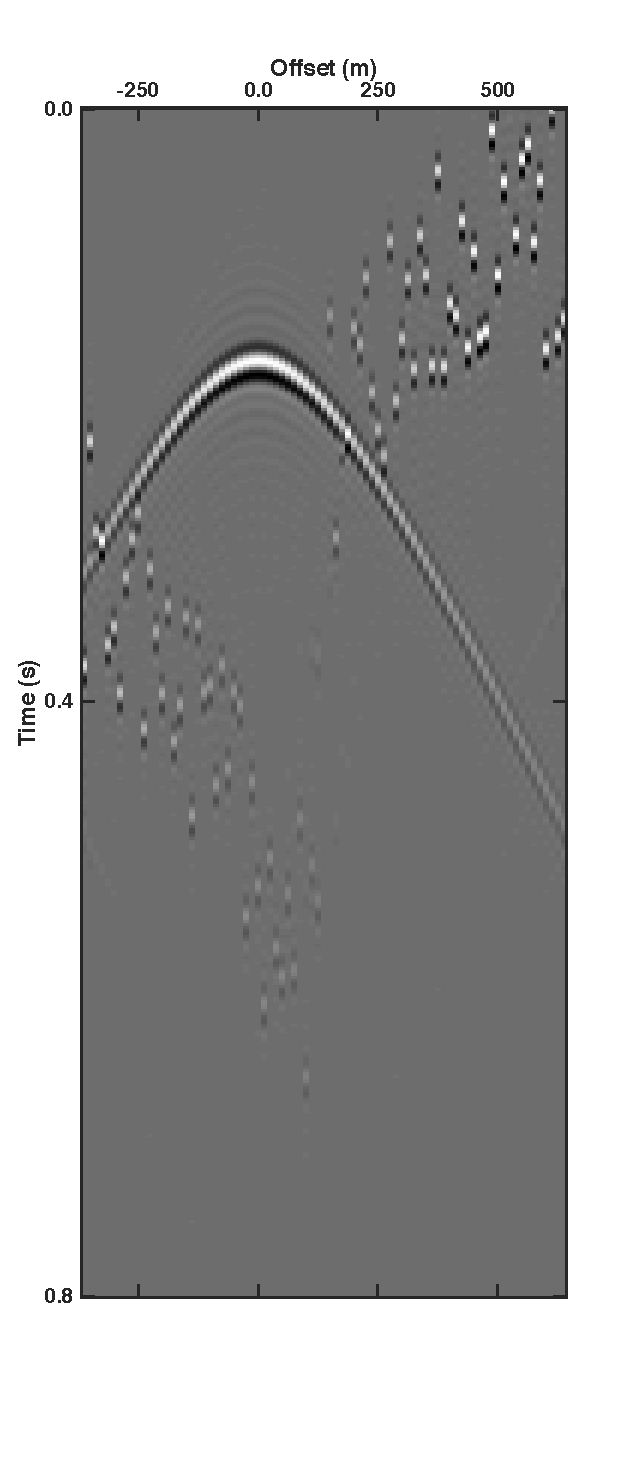
\includegraphics[width=\textwidth]{Plots/Mahdad/1iter/DeblendedCRG_rec30}	
		\caption{1 Iteration}
		\label{fig:Ch-Theory-DeblendedCRG1}
	\end{subfigure}
	%
	\centering
	\begin{subfigure}[t]{0.25\textwidth}
		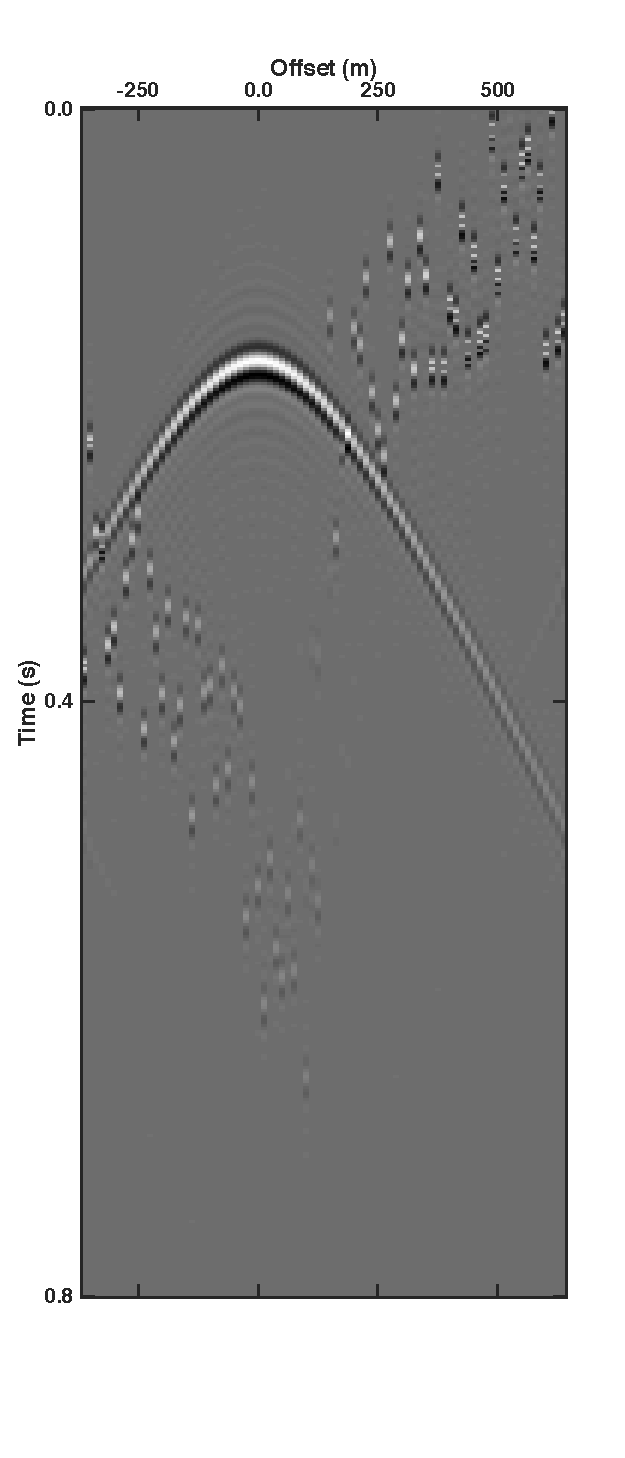
\includegraphics[width=\textwidth]{Plots/Mahdad/5iter/DeblendedCRG_rec30}	
		\caption{5 Iterations}
		\label{fig:Ch-Theory-DeblendedCRG5}
	\end{subfigure}
	%
	\begin{subfigure}[t]{0.25\textwidth}
		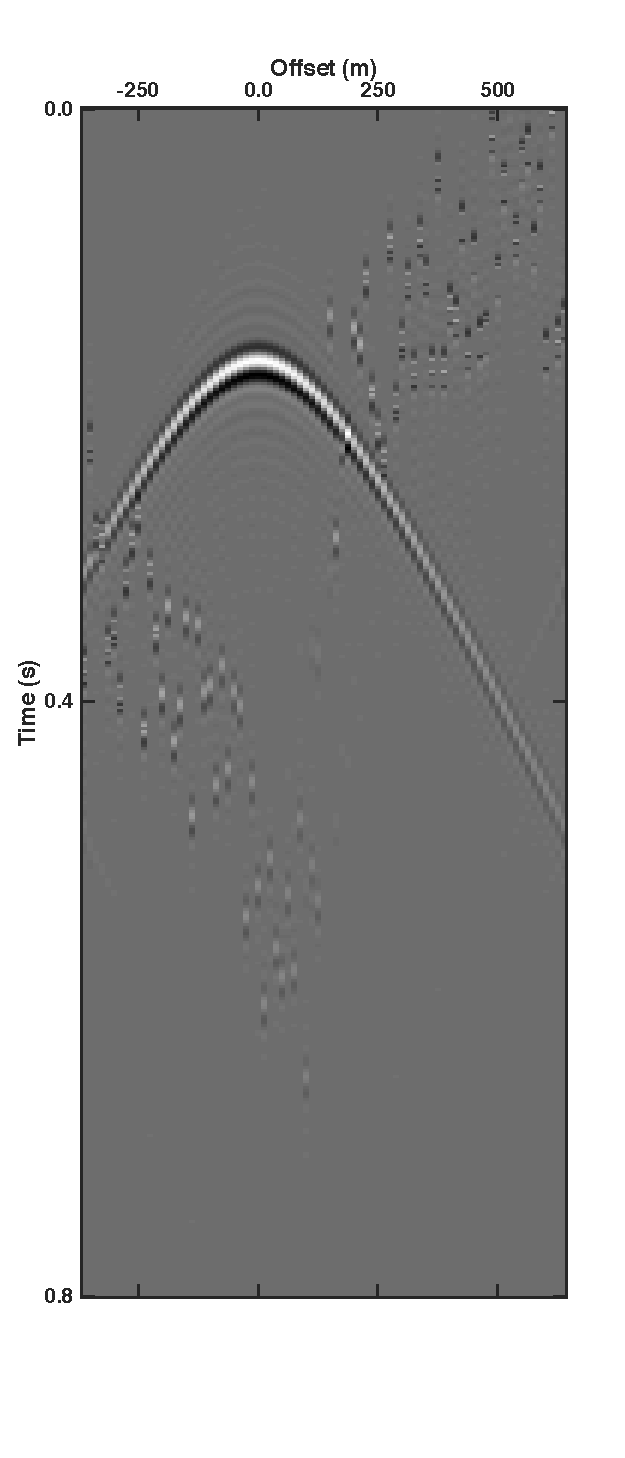
\includegraphics[width=\textwidth]{Plots/Mahdad/10iter/DeblendedCRG_rec30}	
		\caption{10 Iterations}
		\label{fig:Ch-Theory-DeblendedCRG10}
	\end{subfigure}
	%
	\begin{subfigure}[t]{0.25\textwidth}
		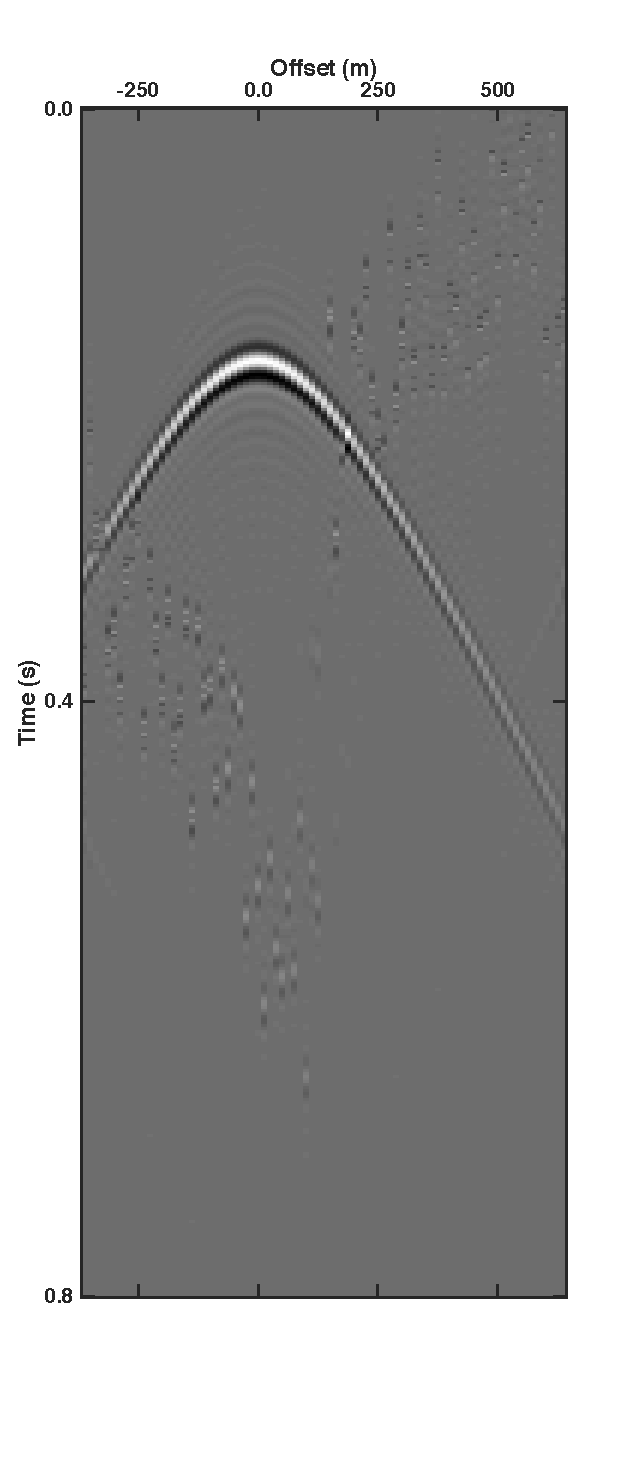
\includegraphics[width=\textwidth]{Plots/Mahdad/15iter/DeblendedCRG_rec30}	
		\caption{15 Iterations}
		\label{fig:Ch-Theory-DeblendedCRG15}
	\end{subfigure}
	%
	\begin{subfigure}[t]{0.25\textwidth}
		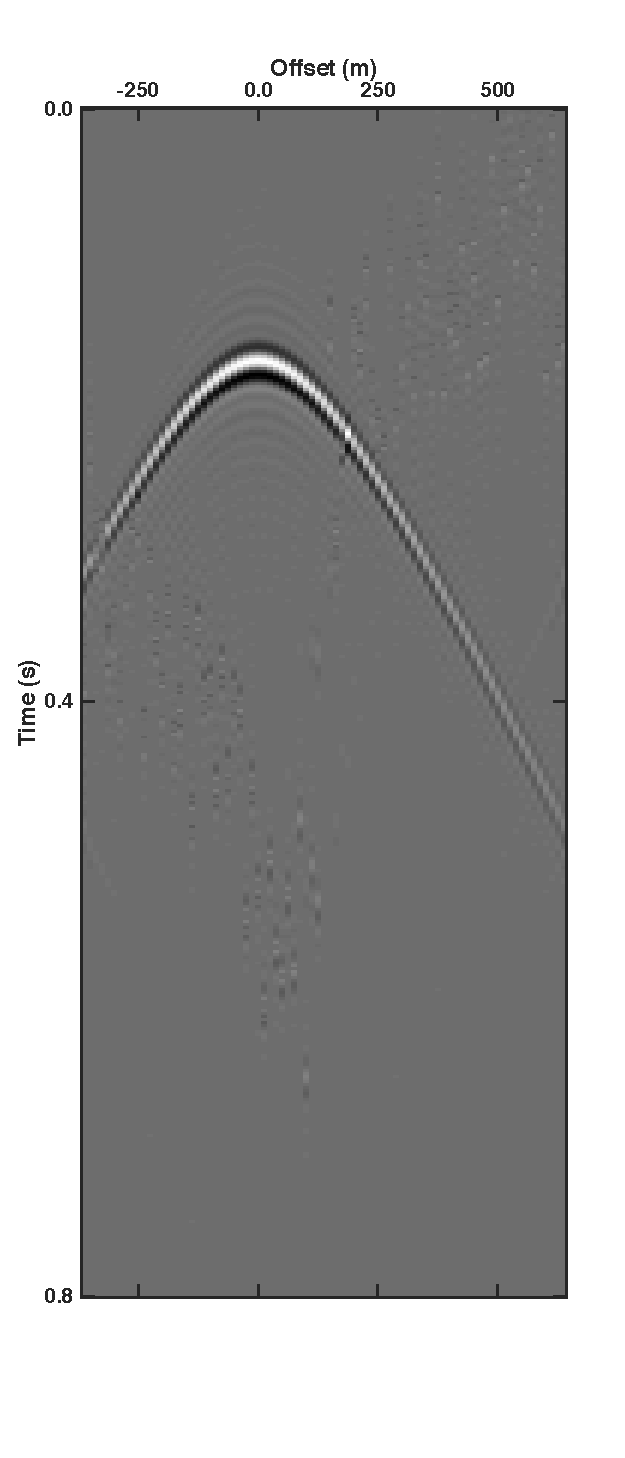
\includegraphics[width=\textwidth]{Plots/Mahdad/20iter/DeblendedCRG_rec30}	
		\caption{20 Iterations}
		\label{fig:Ch-Theory-DeblendedCRG20}
	\end{subfigure}
	%
	\begin{subfigure}[t]{0.25\textwidth}
		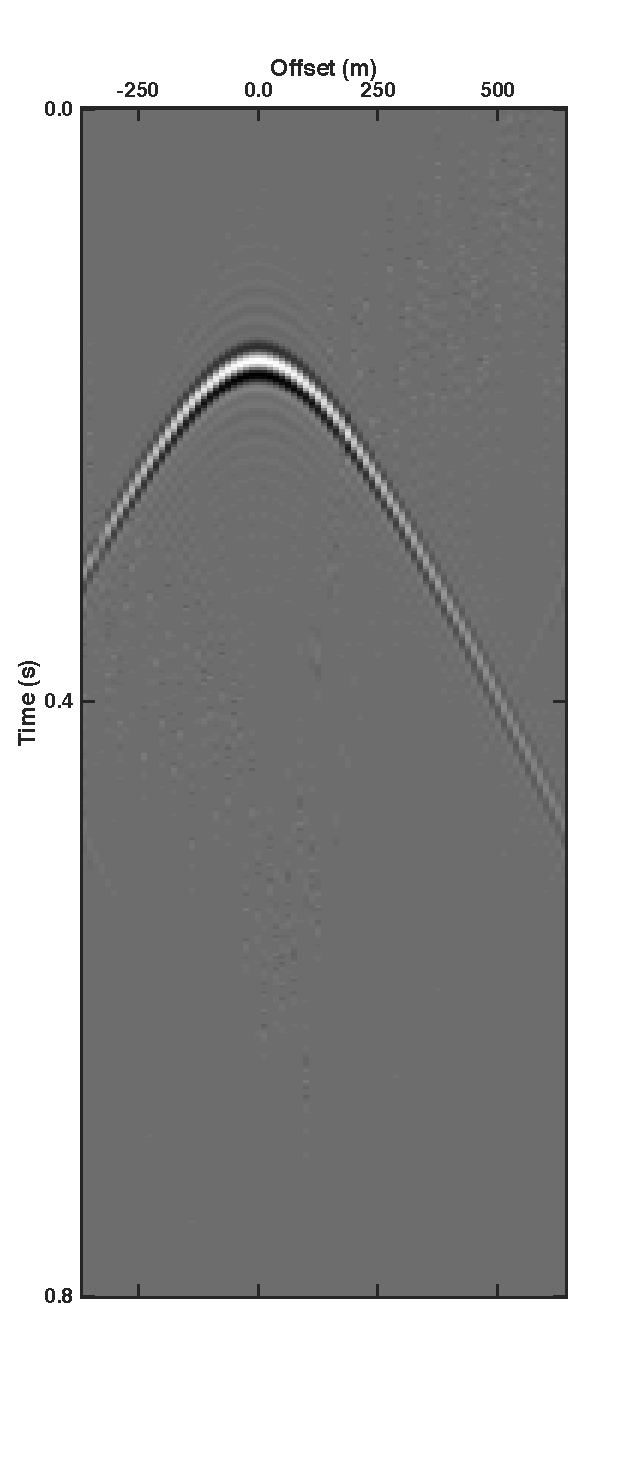
\includegraphics[width=\textwidth]{Plots/Mahdad/25iter/DeblendedCRG_rec30}	
		\caption{25 Iterations}
		\label{fig:Ch-Theory-DeblendedCRG25}
	\end{subfigure}
	\caption{Common receiver gather of the estimated data after 1, 5, 10, 15, 20 and 25 iterations.}
	\label{fig:Ch-Theory-EstimatedData}

\end{figure}

\FloatBarrier

\section{Analysis of the Blending Matrix} \label{sec:BlendingMatrix}

In order to optimize the blended acquisition design, one must understand the properties of the blending matrix $\mathbf{\Gamma}$ and its influence on the deblending performance.

The blending matrix $\mathbf{\Gamma}$ determines the pseudo-deblended data,

\begin{equation}
	\mathbf{ P_{ps} } = \mathbf{P \Gamma \Gamma ^H},
	\label{eq:Ch-Theory-Pseudo-Deblended-Data}
\end{equation}

which is a superposition of the unblended data, $\mathbf{P}$, and the source interference, $\mathbf{N}$,

\begin{equation}
	\mathbf{P}_{ps} = \mathbf{P} + \mathbf{N}.
	\label{eq:Ch-Theory-PseudoSuperposition}
\end{equation}

The more incoherent the source interference, $\mathbf{N}$, the better it can be removed by noise filters.

In the following the effect of the blending matrix, $\mathbf{\Gamma}$, on the product $\mathbf{\Gamma \Gamma}^H$ and on the pseudo-deblended data is analyzed. For simplicity, it is assumed that the blending matrix, $\mathbf{\Gamma}$, only contains phase shift terms, $\mathrm{e}^{-j \omega \Delta t}$, with an amplitude equal to 1 or 0. It is also assumed that each source is fired only once, unlike e.g. the shot repetition case \citep{Sixue}.

Each row of $\mathbf{\Gamma}$ represents a source $k$ and each column of $\mathbf{\Gamma ^H}$ represents a source $l$ with a complex conjugated phase term (see Figure \ref{fig:Ch-Theory-GGH}). Hence, each element $g_{kl}$ of the matrix $\mathbf{\Gamma \Gamma}^H$ is the dot product between the $k^{th}$ source and the complex conjugate of the $l^{th}$ source.

\begin{figure}
	\centering
	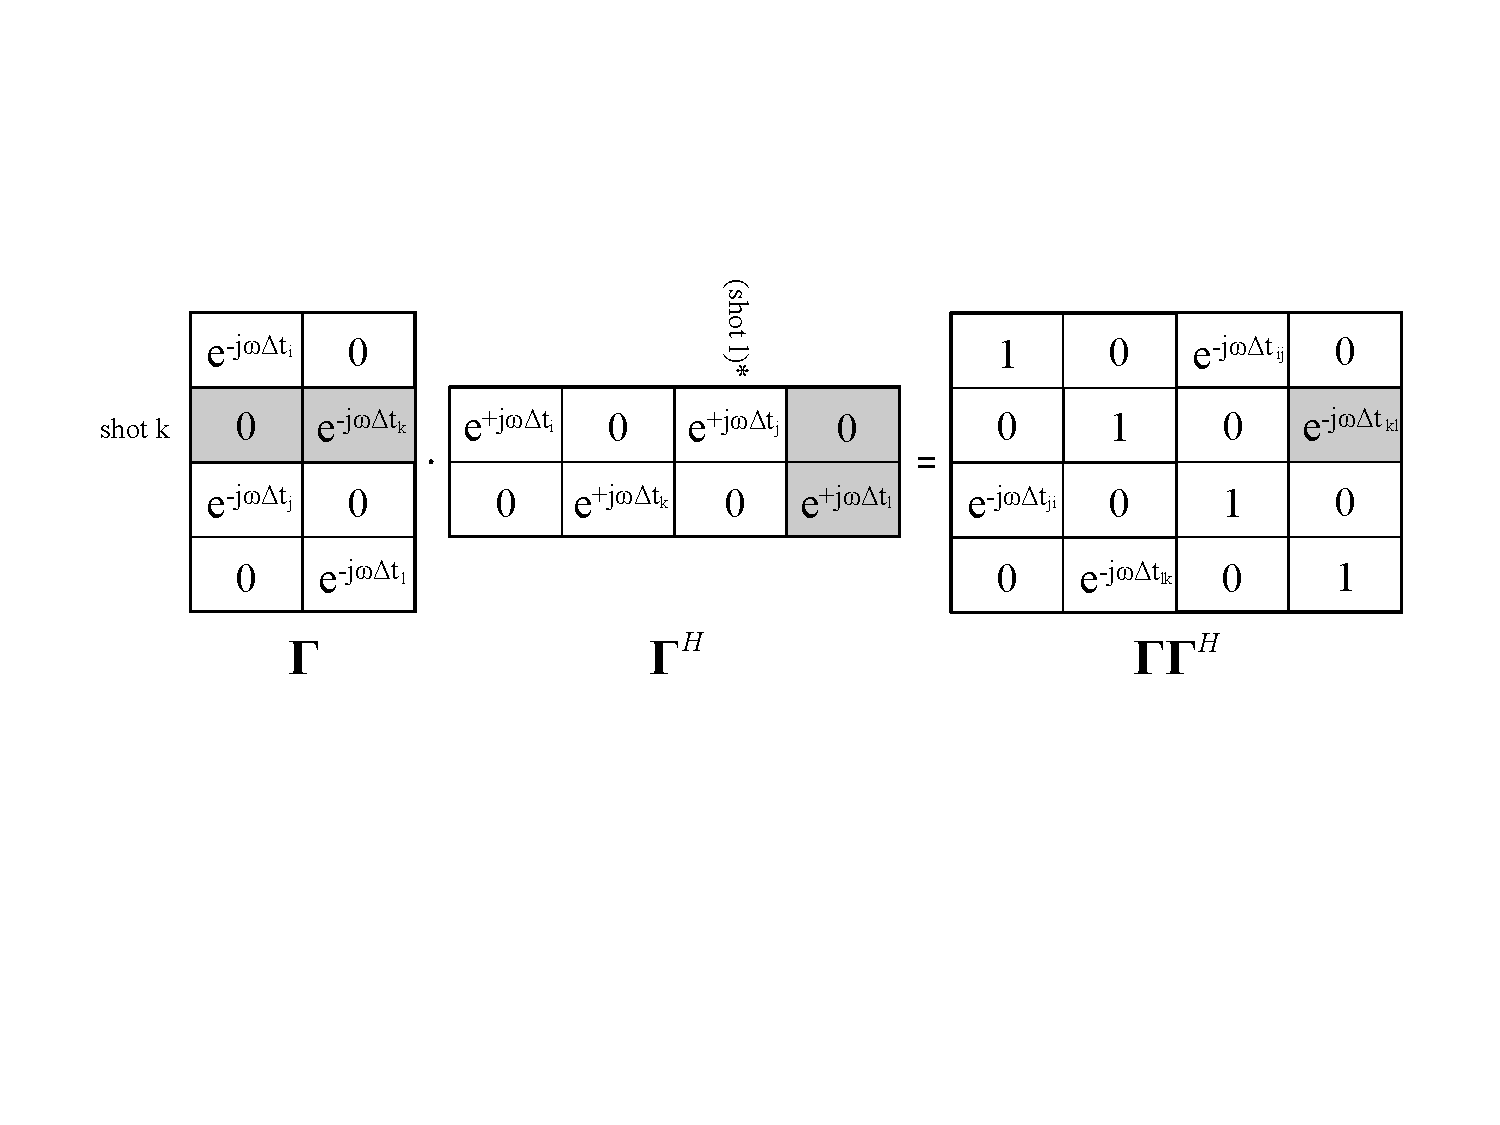
\includegraphics[width = \textwidth]{Plots/GGH}
	\caption{Illustration of the matrix product, $\mathbf{\Gamma \Gamma}^H$. In this notation $\Delta t_k$ refers to the phase shift of the source $k$, and $\Delta t_{kl}$ refers to the phase shift between the sources $k$ and $l$, $\Delta t_{kl} = \Delta t_k - \Delta t_l$.}
	\label{fig:Ch-Theory-GGH}
\end{figure}

Consequently, an element $g_{kl}$ of the product $\mathbf{\Gamma \Gamma}^H$ represents the overlap of the sources $k$ and $l$ for all experiments. The main diagonal of $\mathbf{\Gamma \Gamma}^H$ refers to the overlap of each source with itself, which of course is perfect and therefore equal to 1. The off diagonal elements of $\mathbf{\Gamma \Gamma}^H$ are either 0 if the associated sources do not overlap, or contain a phase shift, $\mathrm{e}^{\, -j \omega \Delta t_{kl}}$.

In equation \ref{eq:Ch-Theory-Pseudo-Deblended-Data} the main diagonal elements of $\mathbf{\Gamma \Gamma}^H$ copy the data matrix, $\mathbf{P}$, while the off-diagonal elements create the source interference, $\mathbf{N}$. If the elements $g_{ik}$ along a sub-diagonal are in phase, they will shift the columns of the data matrix and apply a coherent phase shift to each of them (see Figure \ref{fig:Ch-Theory-PseudoCRG-CoherentDelay}). Instead if the elements $g_{ik}$ along a sub-diagonal are out of phase, they will shift the columns of the data matrix and distort the phase of each column (see Figure \ref{fig:Ch-Theory-PseudoCRG-IncoherentDelay}). 

Figure \ref{fig:Ch-Theory-PseudoCRG-FK-CoherentDelay} and \ref{fig:Ch-Theory-PseudoCRG-FK-IncoherentDelay} display the $f$-$k$-spectra of the pseudo-blended data for constant and random firing time delays respectively. In the case of constant firing time delays almost all of the energy maps in the signal cone. In the case of random firing time delays a significant part of the energy maps outside of the signal cone. Therefore, the coherency constraint requires random firing delays.  

\begin{figure}
	\centering
	\begin{subfigure}[b]{0.3\textwidth}
		\centering
		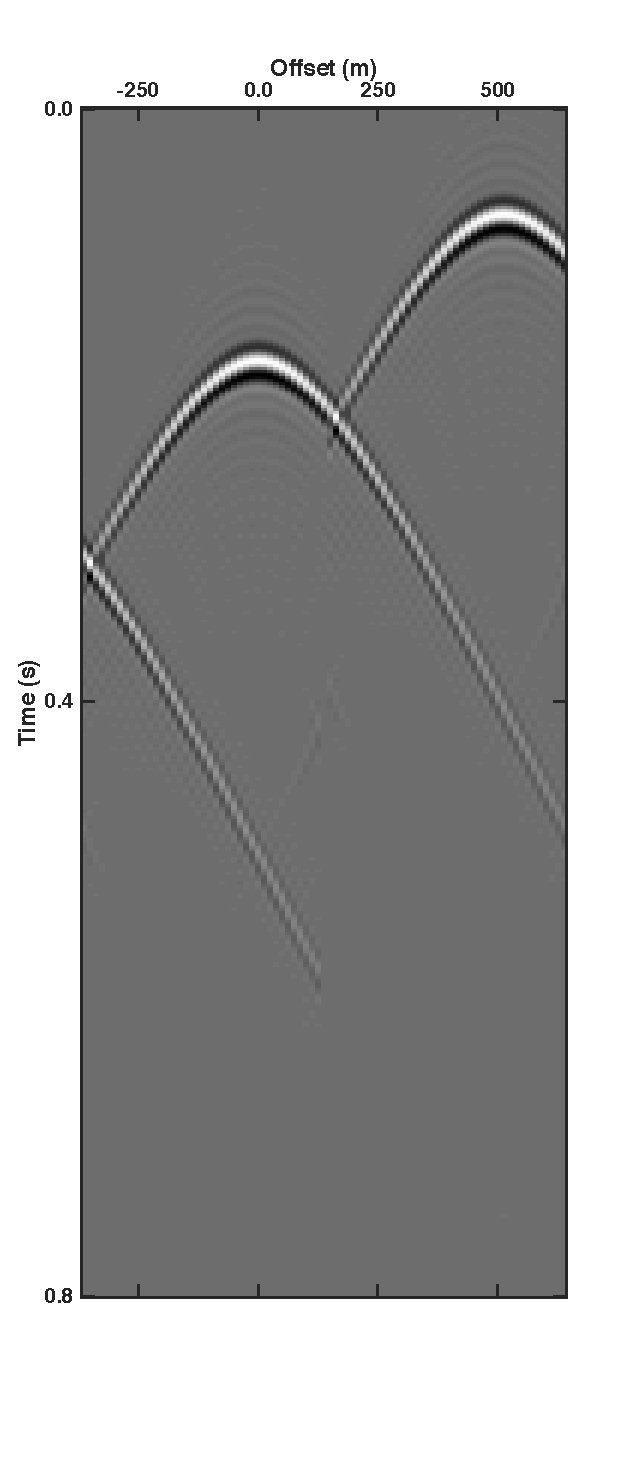
\includegraphics[width = \textwidth]{Plots/Mahdad/25iter/TimeDelay/Pseudo-DeblendedCRG_rec30_coh}
		\caption{}
		\label{fig:Ch-Theory-PseudoCRG-CoherentDelay}
	\end{subfigure}
	%
	\centering
	\begin{subfigure}[b]{0.3\textwidth}
		\centering
		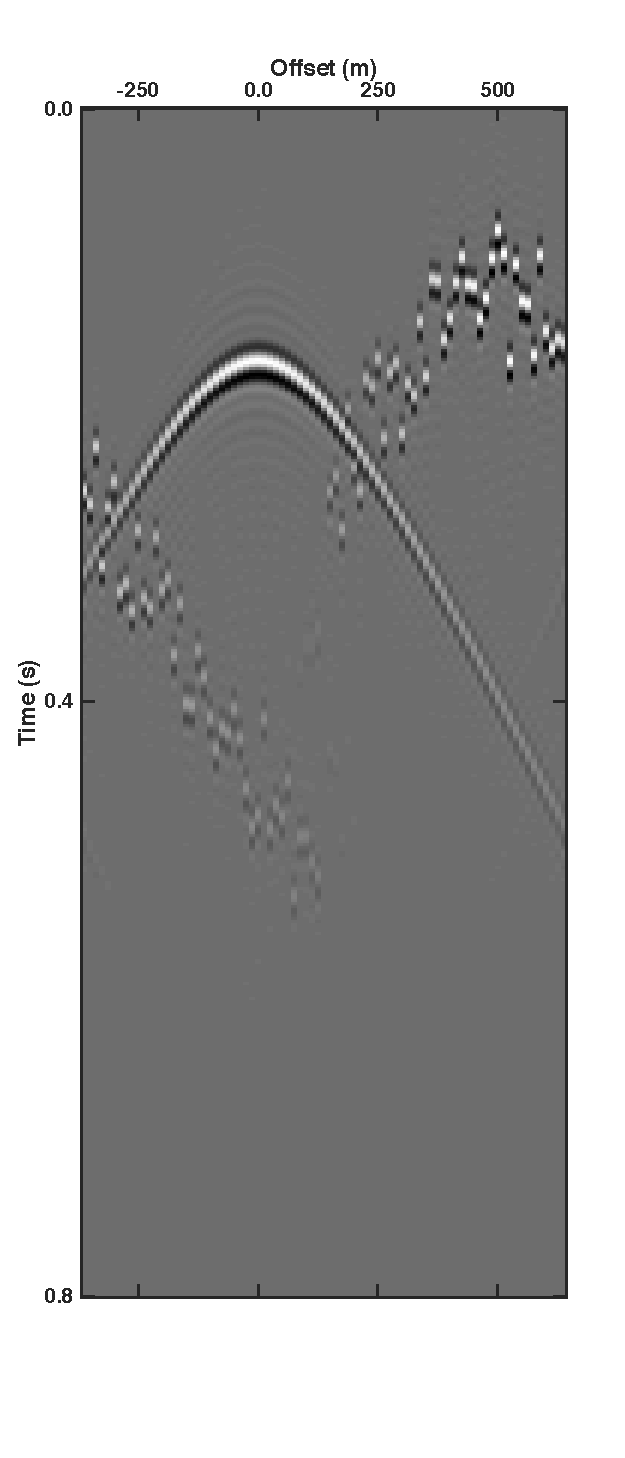
\includegraphics[width = \textwidth]{Plots/Mahdad/25iter/TimeDelay/Pseudo-DeblendedCRG_rec30}
		\caption{}
		\label{fig:Ch-Theory-PseudoCRG-IncoherentDelay}
	\end{subfigure}
	%
	\centering
	\begin{subfigure}[b]{0.3\textwidth}
	
		\centering
		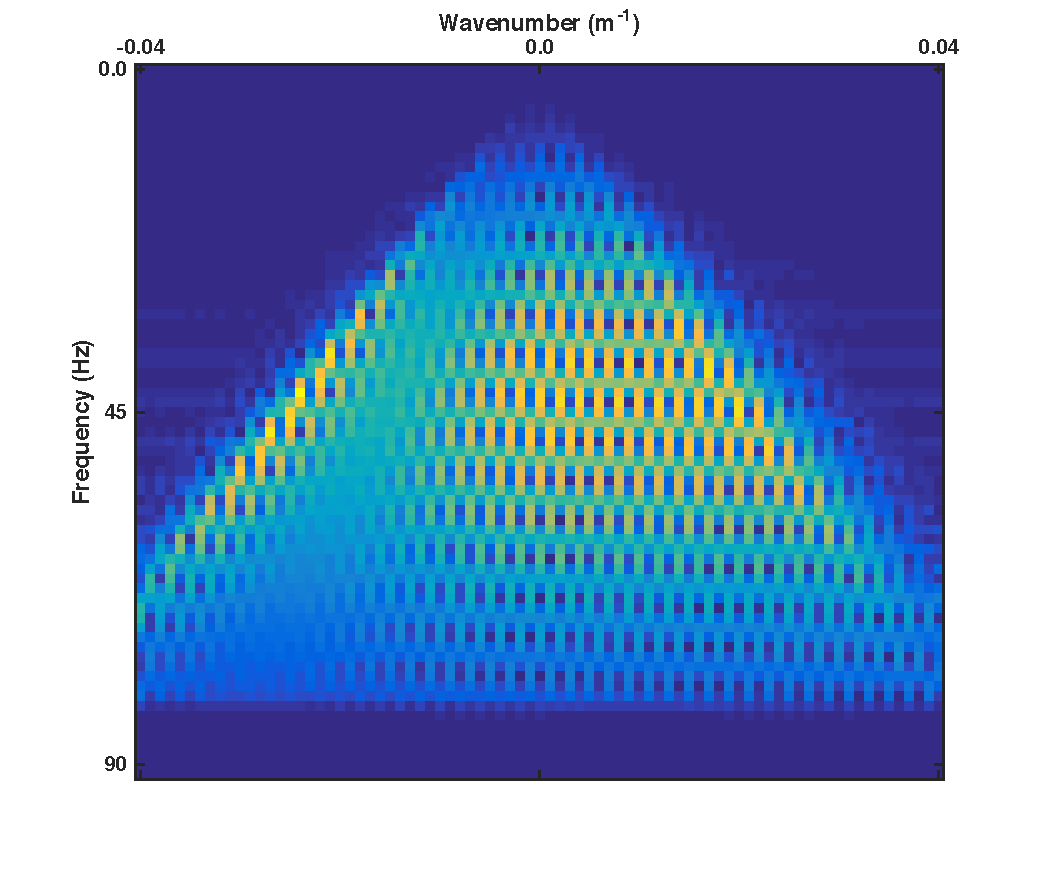
\includegraphics[width = \textwidth]{Plots/Mahdad/25iter/TimeDelay/FK-Pseudo-deblendedCRG_rec30_coh}
		\caption{}
		\label{fig:Ch-Theory-PseudoCRG-FK-CoherentDelay}
		
		\par\bigskip
		
		\centering
		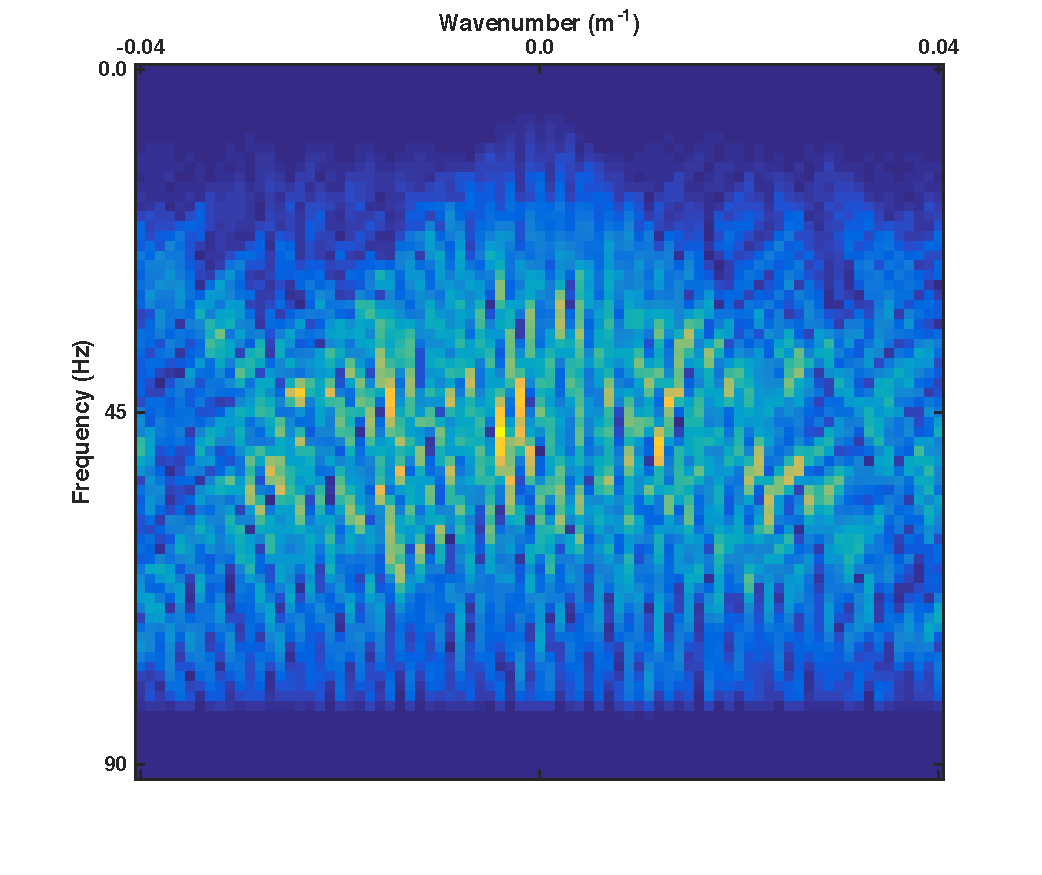
\includegraphics[width = \textwidth]{Plots/Mahdad/25iter/TimeDelay/FK-Pseudo-deblendedCRG_rec30}
		\caption{}
		\label{fig:Ch-Theory-PseudoCRG-FK-IncoherentDelay}
		
	\end{subfigure}
	
	\caption{Comparison of the pseudo-deblended receiver gather for (a) constant firing time delays of \SI{100}{\milli\second}, and (b) random firing time delays between \SI{0}{\milli\second} and \SI{100}{\milli\second}. (c) and (d) show the $f$-$k$-spectra of (a) and (b) respectively.}
	\label{fig:Ch-Theory-PseudoCRG-IncoherencyEffect}

\end{figure}

\begin{figure}
	\centering
	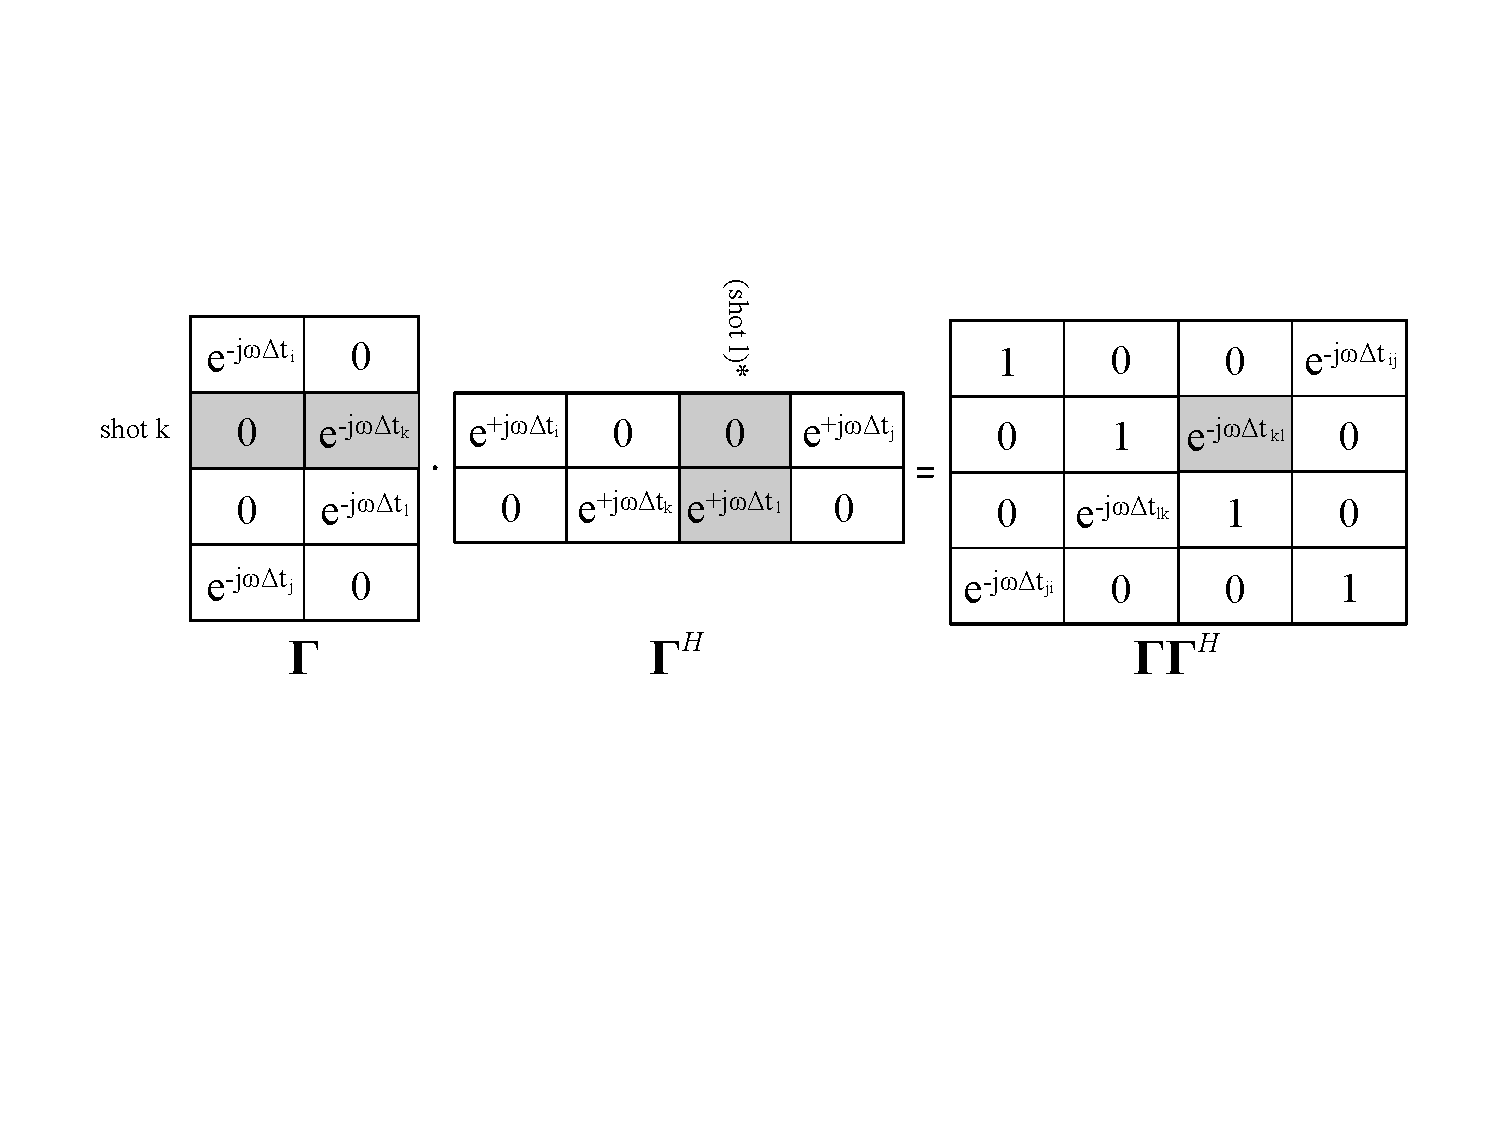
\includegraphics[width=\textwidth]{Plots/GGH_x}
	\caption{The blending matrix, $\mathbf{\Gamma}$, is obtained by interchanging the $3^{rd}$ and $4^{th}$ row of the blending matrix in Figure \ref{fig:Ch-Theory-GGH}. In acquisition this is equivalent to moving source 3 to experiment 2, and source 4 to experiment 1. A random permutation of the rows of the blending matrix spreads the off-diagonal elements of the matrix product, $\mathbf{\Gamma\Gamma}^H$. The elements are not assembled on the sub-diagonals anymore.}
	\label{fig:Ch-Theory-GGHx}
\end{figure}

\begin{comment}
In order to generate incoherent source interference, $\mathbf{N}$, it is therefore favorable if the elements $a_{ik}$ of each lower or upper diagonal are out of phase. For example, considering the $n^{th}$ upper or lower diagonal of the matrix $\mathbf{\Gamma \Gamma}^H$ this observation translates to the acquisition as follows: All source pairs, which are $n$ sources apart from each other, must be fired incoherently. The incoherent firing is realized by delaying blended sources with a random time delay.
\end{comment}

Of course, the degree of incoherency of the source interference, $\mathbf{N}$, also depends on whether the sources blended in an experiment are selected randomly, or in a spatially coherent pattern. For example, one expects the source interference to be more incoherent if in each experiment randomly picked sources are blended, than if in each experiment adjacent sources are blended (see Figure \ref{fig:Ch-Theory-GGHx}).

In 2D blending only adjacent sources can be blended, thus, the blended sources cannot be selected randomly. This changes when blending is extended to 3D: Within the crossline direction sources can be selected randomly and blended. 

\todo[inline]{This might need some extra explanation and plot!}

\begin{comment}

In terms of the blending matrix $\mathbf{\Gamma}$ a spatially incoherent firing pattern means that the rows, i.e. the sources, are shuffled randomly. As a consequence the off-diagonal elements of the matrix product $\mathbf{\Gamma \Gamma}^H$ are reordered randomly. This shuffling process can help to further distort the phase of the interfering sources. However, if the maximum allowed time delay between blended sources is aready large the spatially incoherent blending pattern will not increase the incoherency of the interfering sources.   

In practice, the maximum allowed firing time delay is limited by the available acquisition time. The spatial distribution of blended sources is constraint by the acquisition design.
	
\end{comment}


\FloatBarrier


    	\chapter{Incoherency} \label{chap:Incoherency}

In this chapter the blending operator is analyzed in greater detail. Then a measure for incoherency will be introduced and the role of incoherency for deblending will be discussed.

\section{Analysis of the Blending Matrix} \label{sec:BlendingMatrix}

In order to optimize the blended acquisition design, one must understand the properties of the blending matrix $\mathbf{\Gamma}$ and its influence on the deblending performance.

The blending matrix $\mathbf{\Gamma}$ determines the pseudo-deblended data,

\begin{equation}
	\mathbf{P}_{ps} = \mathbf{P \Gamma \Gamma}^H,
	\label{eq:Ch-Theory-Pseudo-Deblended-Data}
\end{equation}

which are a superposition of the unblended data, $\mathbf{P}$, and the blending noise, $\mathbf{N}$,

\begin{equation}
	\mathbf{P}_{ps} = \mathbf{P} + \mathbf{N}.
	\label{eq:Ch-Theory-PseudoSuperposition}
\end{equation}

The more incoherent the blending noise, $\mathbf{N}$, the better it can be removed by noise filters.

In the following the effect of the blending matrix, $\mathbf{\Gamma}$, on the matrix product $\mathbf{\Gamma \Gamma}^H$ and on the pseudo-deblended data is analyzed. For simplicity, it is assumed that all shots are equal in strength and fire the same signature into the earth. This means that the blending matrix, $\mathbf{\Gamma}$, only contains phase shift terms, $\mathrm{e}^{-j \omega \Delta t}$, with an amplitude equal to 1 or 0. It is also assumed that each shot is fired only once, unlike e.g. the shot repetition case \citep{Sixue}.

Each row of $\mathbf{\Gamma}$ represents a shot $k$, and each column of $\mathbf{\Gamma}^H$ represents a shot $l$ with a complex conjugated phase term (see Figure \ref{fig:Ch-Theory-GGH}). Hence, each element $g_{kl}$ of the matrix $\mathbf{\Gamma \Gamma}^H$ is the dot product between the $k^{th}$ shot and the complex conjugate of the $l^{th}$ shot.

\begin{figure}
	\centering
	\includegraphics[width = \textwidth]{Plots/GGH_v2}
	\caption{Illustration of the matrix product, $\mathbf{\Gamma \Gamma}^H$. In this notation $\Delta t_k$ refers to the phase shift of the shot $k$, and $\Delta t_{kl}$ refers to the phase shift between the shots $k$ and $l$, $\Delta t_{kl} = \Delta t_k - \Delta t_l$.}
	\label{fig:Ch-Theory-GGH}
\end{figure}

Consequently, an element $g_{kl}$ of the matrix product $\mathbf{\Gamma \Gamma}^H$ represents the overlap of the shots $k$ and $l$ for all experiments. The main diagonal of $\mathbf{\Gamma \Gamma}^H$ refers to the overlap of each shot with itself, which of course is perfect and therefore equal to 1. The off diagonal elements of $\mathbf{\Gamma \Gamma}^H$ are either 0 if the associated shots do not overlap, or contain a phase shift, $\mathrm{e}^{\, -j \omega \Delta t_{kl}}$.

\subsection*{Temporal incoherency}

In the following the term "sub-diagonal" will be used to refer to an arbitrary diagonal of the matrix $\mathbf{\Gamma \Gamma}^H$. For example, the $d^{th}$ sub-diagonal includes all the matrix elements $g_{ij}$, which fulfill the condition;

\begin{equation}
	j -i = d.
	\label{eq:Ch-Incoherency-Subdiagonal}
\end{equation}

In equation \ref{eq:Ch-Theory-Pseudo-Deblended-Data} the main diagonal elements of $\mathbf{\Gamma \Gamma}^H$ copy the data matrix, $\mathbf{P}$, while the off-diagonal elements create the blending noise, $\mathbf{N}$. In case of a coherent firing time delay the elements along a sub-diagonal $d$ are in phase. This means that the sub-diagonal elements will shift the columns of the data matrix and apply a coherent phase shift to each of them resulting in the pseudo-deblended receiver gather shown in Figure \ref{fig:Ch-Theory-PseudoCRG-CoherentDelay}. Instead if the elements $g_{ij}$ along a sub-diagonal $d$ are out of phase, they will shift the columns of the data matrix and distort the phase of each column (see Figure \ref{fig:Ch-Theory-PseudoCRG-IncoherentDelay}). 

Figure \ref{fig:Ch-Theory-PseudoCRG-FK-CoherentDelay} and \ref{fig:Ch-Theory-PseudoCRG-FK-IncoherentDelay} display the $f$-$k$-spectra of the pseudo-blended data for constant firing time delays and random firing time delays respectively. In the case of constant firing time delays almost all of the energy maps in the signal cone. In the case of random firing time delays a significant part of the energy maps outside of the signal cone. Therefore, the coherency constraint requires random firing time delays. 

In this thesis the random firing time delays are referred to as temporal incoherency.  

\begin{figure}
	\centering
	\begin{subfigure}[b]{0.3\textwidth}
		\centering
		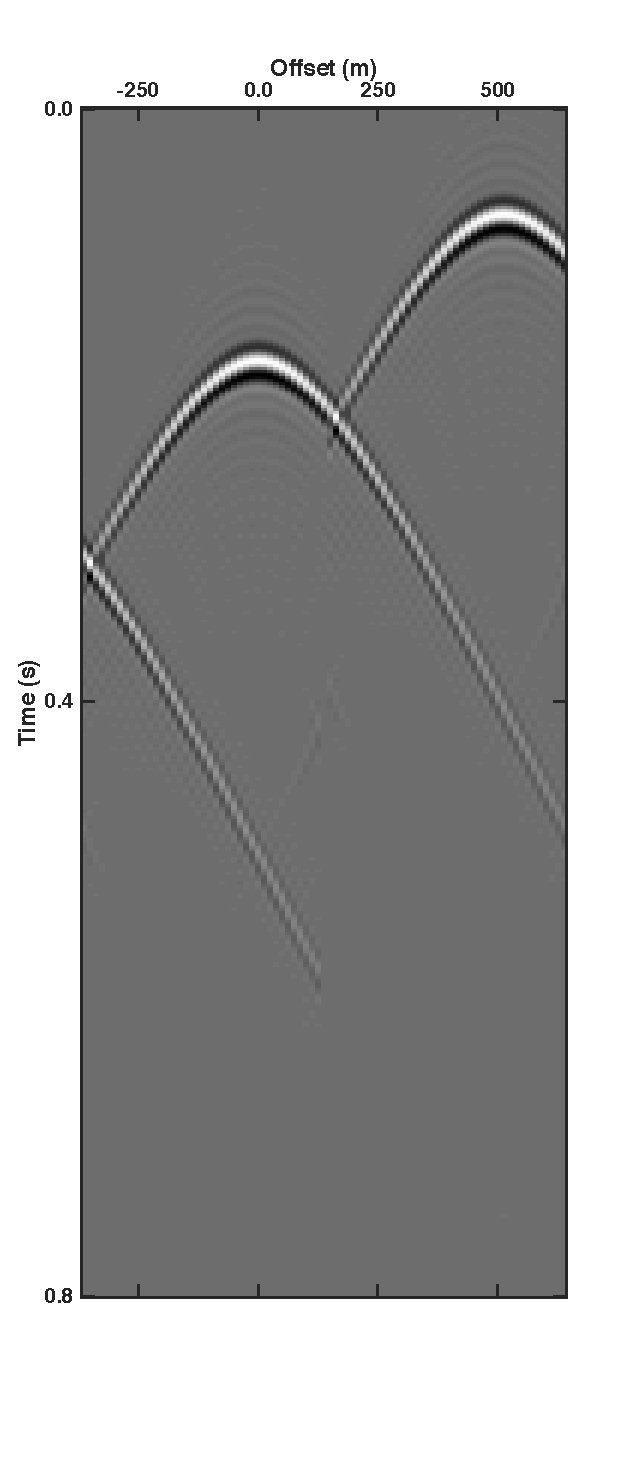
\includegraphics[width = \textwidth]{Plots/Mahdad/25iter/TimeDelay/Pseudo-DeblendedCRG_rec30_coh}
		\caption{}
		\label{fig:Ch-Theory-PseudoCRG-CoherentDelay}
	\end{subfigure}
	%
	\centering
	\begin{subfigure}[b]{0.3\textwidth}
		\centering
		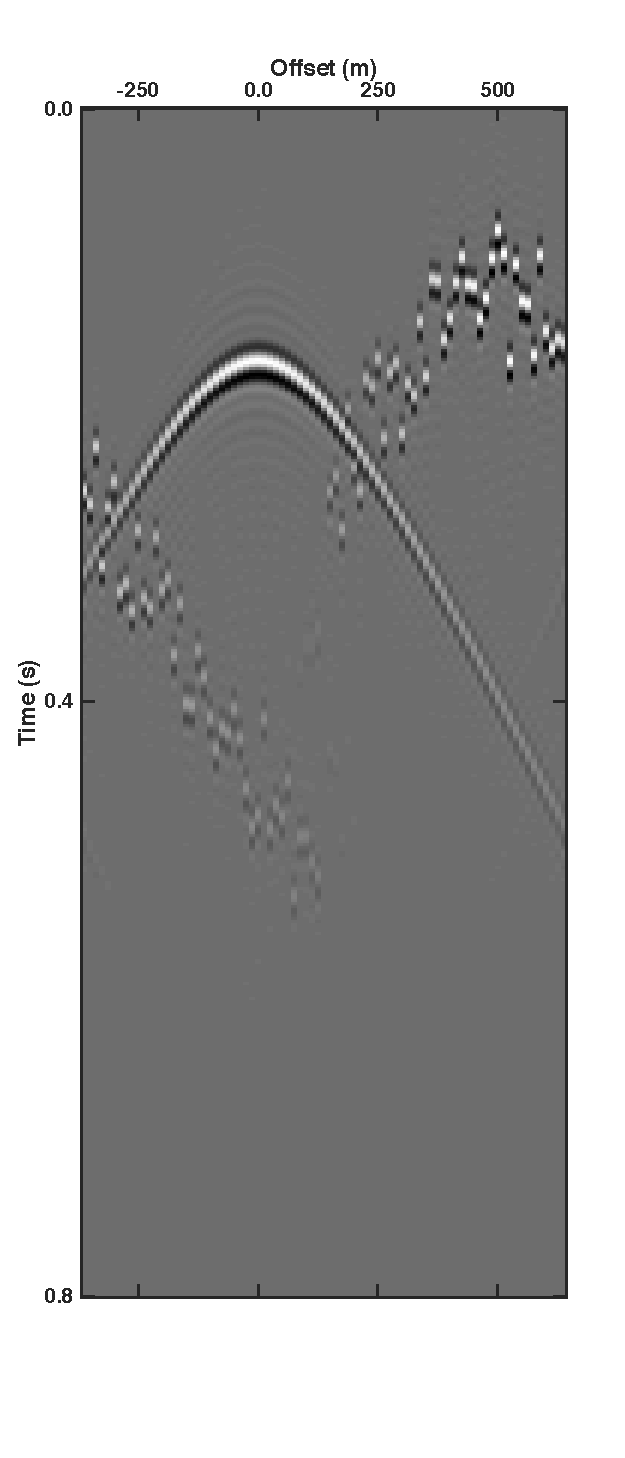
\includegraphics[width = \textwidth]{Plots/Mahdad/25iter/TimeDelay/Pseudo-DeblendedCRG_rec30}
		\caption{}
		\label{fig:Ch-Theory-PseudoCRG-IncoherentDelay}
	\end{subfigure}
	%
	\centering
	\begin{subfigure}[b]{0.3\textwidth}
	
		\centering
		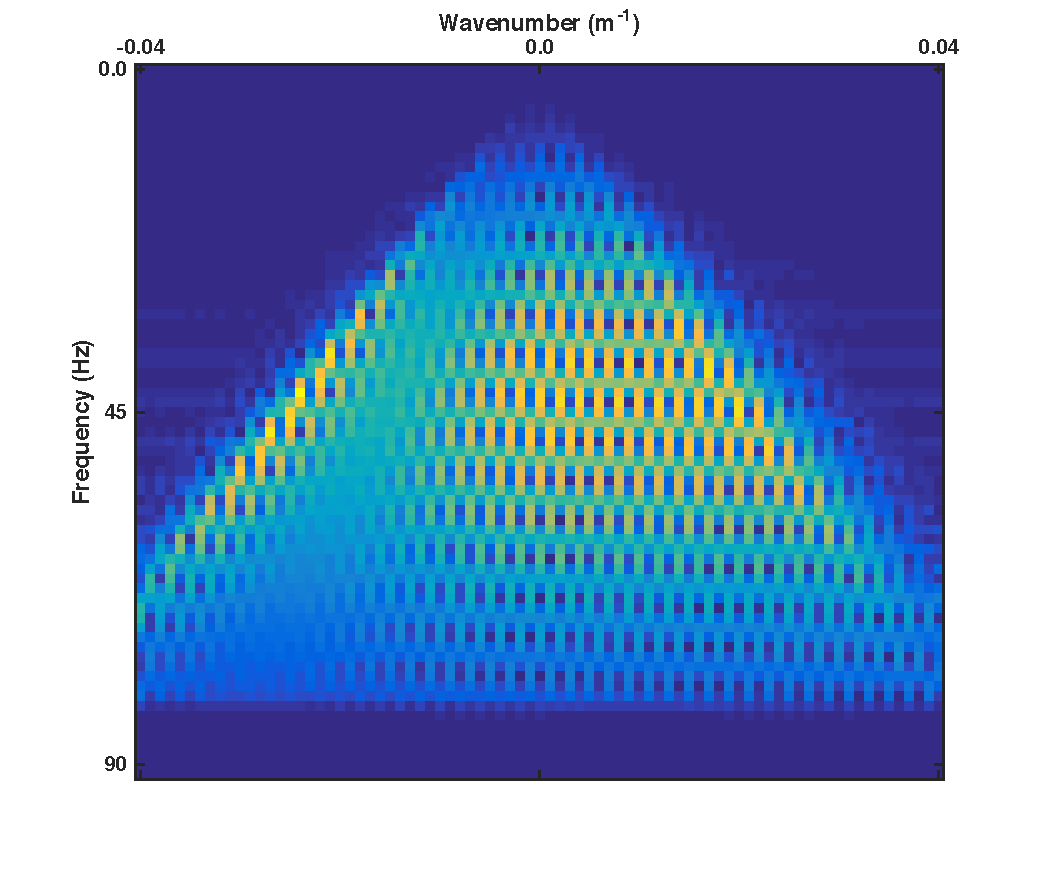
\includegraphics[width = \textwidth]{Plots/Mahdad/25iter/TimeDelay/FK-Pseudo-deblendedCRG_rec30_coh}
		\caption{}
		\label{fig:Ch-Theory-PseudoCRG-FK-CoherentDelay}
		
		\par\bigskip
		
		\centering
		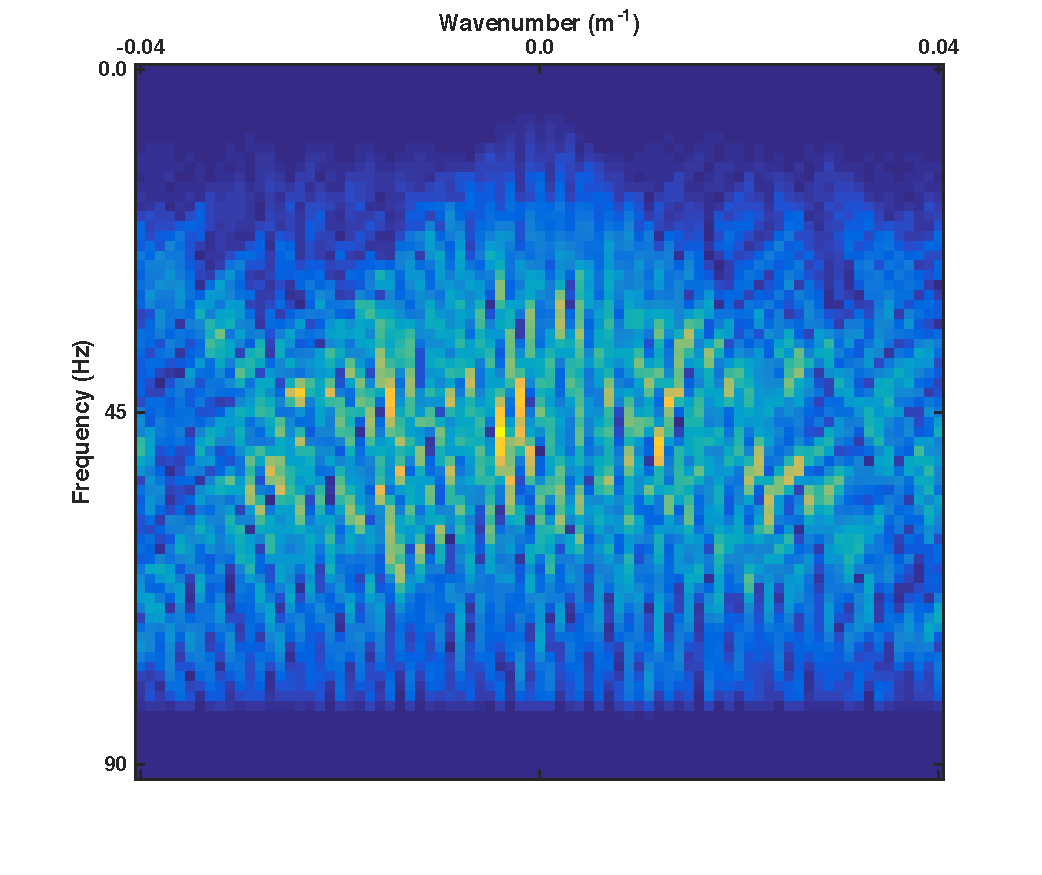
\includegraphics[width = \textwidth]{Plots/Mahdad/25iter/TimeDelay/FK-Pseudo-deblendedCRG_rec30}
		\caption{}
		\label{fig:Ch-Theory-PseudoCRG-FK-IncoherentDelay}
		
	\end{subfigure}
	
	\caption{Comparison of the pseudo-deblended receiver gather for (a) constant firing time delays of \SI{100}{\milli\second}, and (b) random firing time delays between \SI{0}{\milli\second} and \SI{100}{\milli\second}. (c) and (d) show the $f$-$k$-spectra of (a) and (b) respectively.}
	\label{fig:Ch-Theory-PseudoCRG-IncoherencyEffect}

\end{figure}

\begin{figure}
	\centering
	\includegraphics[width=\textwidth]{Plots/GGH_x_v2}
	\caption{The blending matrix, $\mathbf{\Gamma}$, is obtained by interchanging the $3^{rd}$ and $4^{th}$ row of the blending matrix in Figure \ref{fig:Ch-Theory-GGH}. In acquisition this is equivalent to moving shot 3 to experiment 2, and shot 4 to experiment 1. A random permutation of the rows of the blending matrix spreads the off-diagonal elements of the matrix product, $\mathbf{\Gamma\Gamma}^H$. The elements are not assembled on the sub-diagonals anymore.}
	\label{fig:Ch-Theory-GGHx}
\end{figure}

\begin{comment}
In order to generate incoherent source interference, $\mathbf{N}$, it is therefore favorable if the elements $a_{ik}$ of each lower or upper diagonal are out of phase. For example, considering the $n^{th}$ upper or lower diagonal of the matrix $\mathbf{\Gamma \Gamma}^H$ this observation translates to the acquisition as follows: All source pairs, which are $n$ sources apart from each other, must be fired incoherently. The incoherent firing is realized by delaying blended sources with a random time delay.
\end{comment}


\subsection*{Spatial incoherency}

Of course, the degree of incoherency of the blending noise, $\mathbf{N}$, also depends on whether the shots blended in an experiment are selected randomly, or in a spatially coherent pattern. For example, one expects the blending noise to be more incoherent if in each experiment randomly picked shots are blended, than if in each experiment adjacent shots are blended, because the interfering shots are now spread over the sub-diagonals (see Figure \ref{fig:Ch-Theory-GGHx}).

In this thesis selecting random shots for an experiment is referred to as spatial incoherency.

In practice in 2D blending shots cannot be blended in a spatially incoherent fashion, at least not in a conventional 2D marine acquisition design. In the chapter \ref{chap:MahdadMethod3d} it will be shown that blending in 3D allows to blend shots spatially incoherent within the crossline direction. 

In this chapter spatial incoherency will be illustrated with 2D synthetic data, where the acquisition design is not constraint by practicability.



\begin{comment}

In terms of the blending matrix $\mathbf{\Gamma}$ a spatially incoherent firing pattern means that the rows, i.e. the sources, are shuffled randomly. As a consequence the off-diagonal elements of the matrix product $\mathbf{\Gamma \Gamma}^H$ are reordered randomly. This shuffling process can help to further distort the phase of the interfering sources. However, if the maximum allowed time delay between blended sources is aready large the spatially incoherent blending pattern will not increase the incoherency of the interfering sources.   

In practice, the maximum allowed firing time delay is limited by the available acquisition time. The spatial distribution of blended sources is constraint by the acquisition design.
	
\end{comment}


\FloatBarrier

\section{Effect of Incoherency}

An incoherent blending pattern is crucial for good deblending performance (see section \ref{sec:BlendingMatrix}). Thus, a measure of incoherency and deblending quality will be introduced. Then, the possibilities of creating an incoherent blending pattern are presented. Finally, the effect of incoherency on the deblending quality will be shown on a synthetic data set.


\subsection*{Incoherency Measure}

\todo[inline]{Move this sentence to the introduction (literature). You might also want to mention the work of the Greek guy Apostolos.\\
In this thesis only the incoherency of the acquisition design is considered. Thus, the blending matrix, $\Gamma$, or more precisely the product $\mathbf{\Gamma \Gamma}^H$ determines the incoherency.}

A measure of incoherency will be introduced in order to analyze the importance of an incoherent blending pattern quantitatively.

In section \ref{sec:BlendingMatrix} it was shown that for an incoherent blending pattern the elements, $\mathrm{e}^{-j \omega \Delta t_{kl}}$, along a sub-diagonal of the matrix product $\mathbf{\Gamma \Gamma}^H$ should be out of phase. Therefore, the phase variability of the sub-diagonal elements will be used to quantify incoherency.

Note that the sub-diagonal elements, $\mathrm{e}^{-j \omega \Delta t_{kl}}$, map in the complex plane on a circle with radius 1 (see Figure \ref{fig:Ch-Results-complex-circle}). 

\begin{figure}
	\centering
	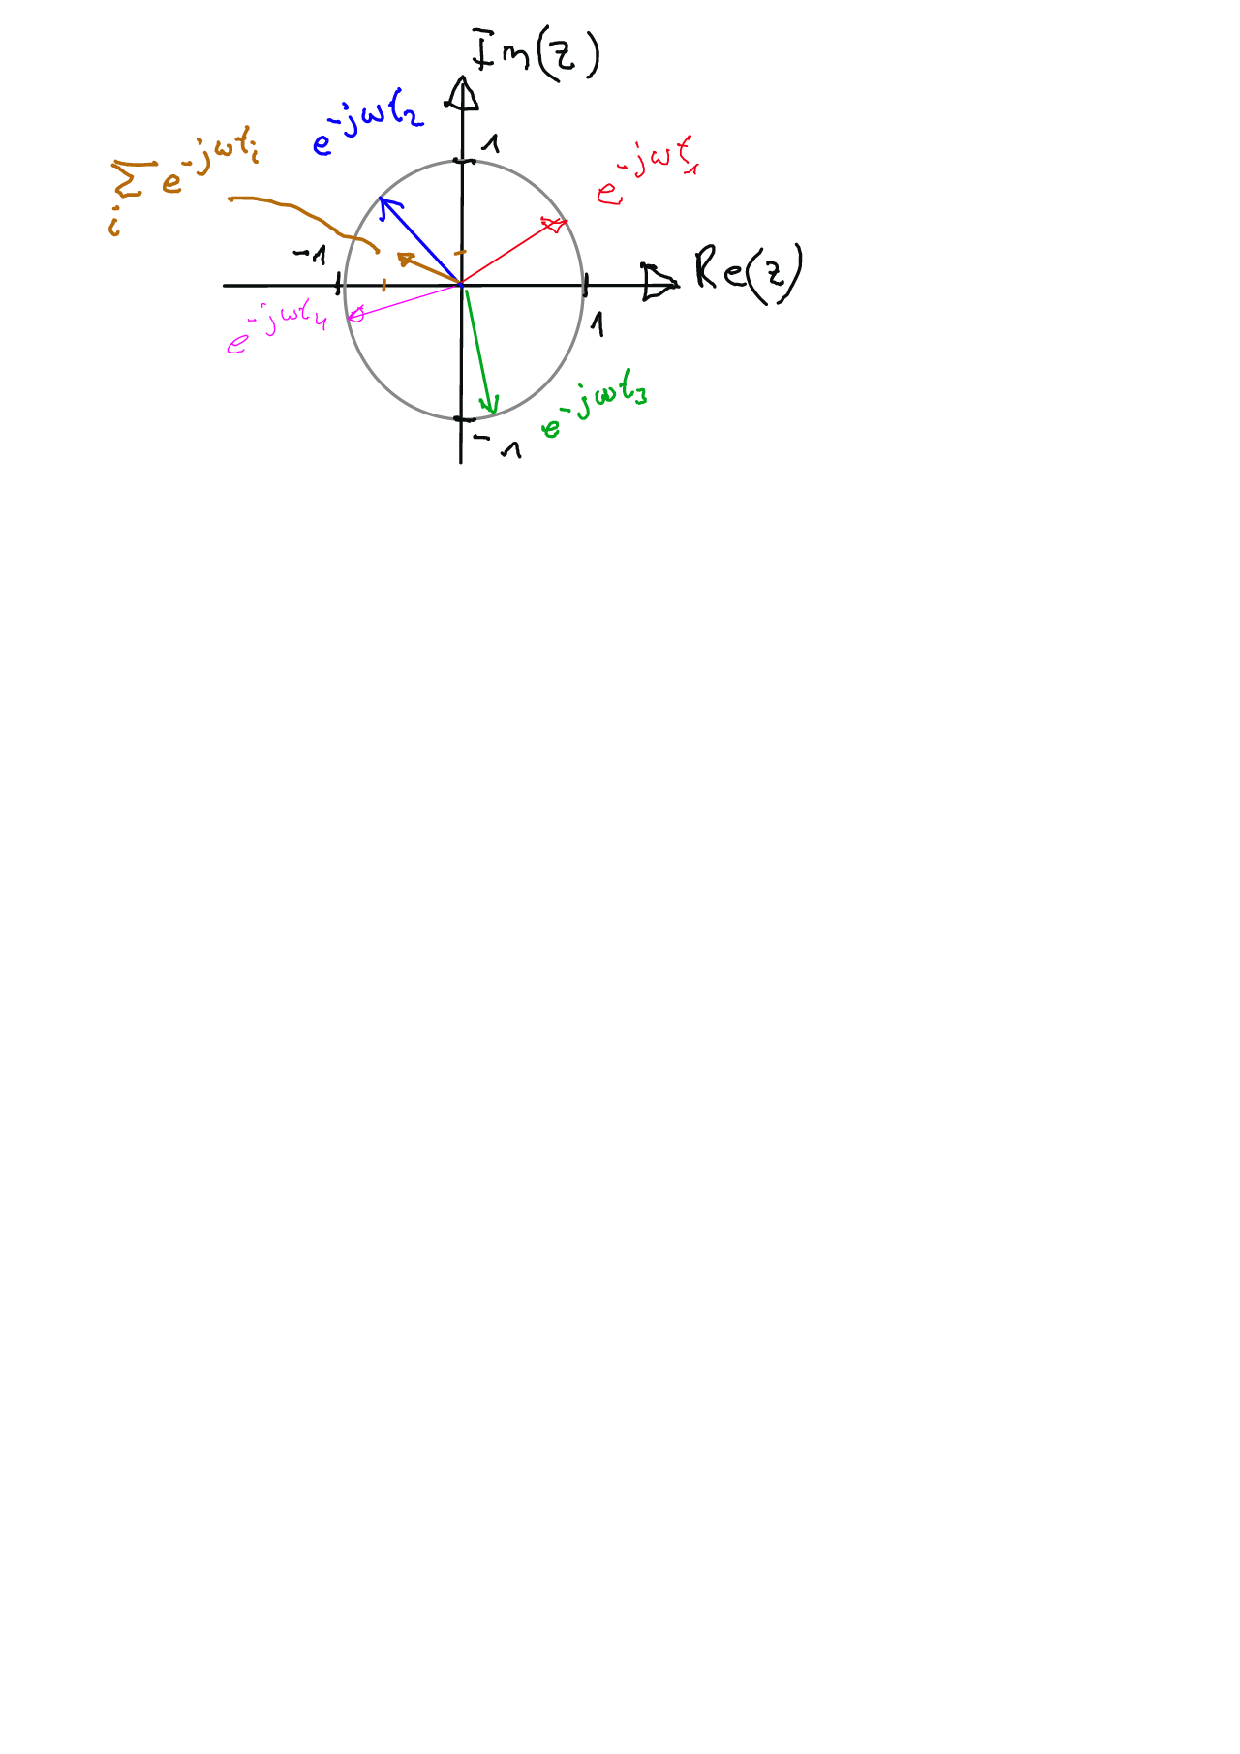
\includegraphics[width = 0.5\textwidth]{Plots/complex-circle}
	\caption{Illustration of the sub-diagonal elements in the complex number plane. The elements have unit length and variable phase. The absolute value of their sum depends on the phase coherency of the elements.}
	\label{fig:Ch-Results-complex-circle}
\end{figure}

The sum of the elements along the $d^{th}$ sub-diagonal can be constructive or destructive, depending on the phase variability. Thus, the absolute value of the sum, $S(d,\omega)$, measures the incoherency of an individual sub-diagonal. The sum, $S(d,\omega)$, is a function of the sub-diagonal $d$ and the frequency component, $\omega$;

%The resulting value is squared in order to put it in terms of energy;

\begin{equation}
	S(d,\omega) = \left| \sum_{j-i=d} \mathbf{\Gamma \Gamma}^H_{ij} (\omega) \right|.
	\label{eq:Ch-Results-incoherency-diagsum}	
\end{equation} 

For example, if all elements are in phase the absolute value of their sum, $S(d,\omega)$, is maximized. The more the elements are out of phase, i.e. the more incoherent they are, the smaller is $S(d,\omega)$. Thus, in case of an incoherent blending pattern $S(d,\omega)$ is small for all sub-diagonals $d$, except for the main diagonal, $d = 0$.  

All frequency components, $\omega$, of $S(d,\omega)$ are summed. The resulting function, $S(d)$, only depends on the sub-diagonal number. Next, each element of $S(d)$ is squared to relate it to energy. 

The incoherency, $\mu$, is quantified by the ratio of the main diagonal and the sum of all sub-diagonals;

\begin{equation}
	\mu = \frac{\left( \; \sum_{\omega}S(d=0,\omega) \; \right)^2}{\sum_{d = 1-Ns}^{Ns-1} \left(\left( \; \sum_{\omega}S(d,\omega) \; \right)^2\right)}
	\label{eq:Ch-Results-incoherency}
\end{equation}





For illustration a blending matrix, $\mathbf{\Gamma}$, is generated and inserted in equation \ref{eq:Ch-Results-incoherency-diagsum}. This yields an output for each sub-diagonal, which is shown in Figure \ref{fig:Ch-Results-Diagonal-Sums}. The spike is caused by the elements on the main diagonal of $\mathbf{\Gamma \Gamma}^H$, which are all equal to 1, i.e. in phase. For a perfectly incoherent blending design the elements on a sub-diagonal cancel and the plot becomes a perfect spike. 


\begin{figure}
	\centering
	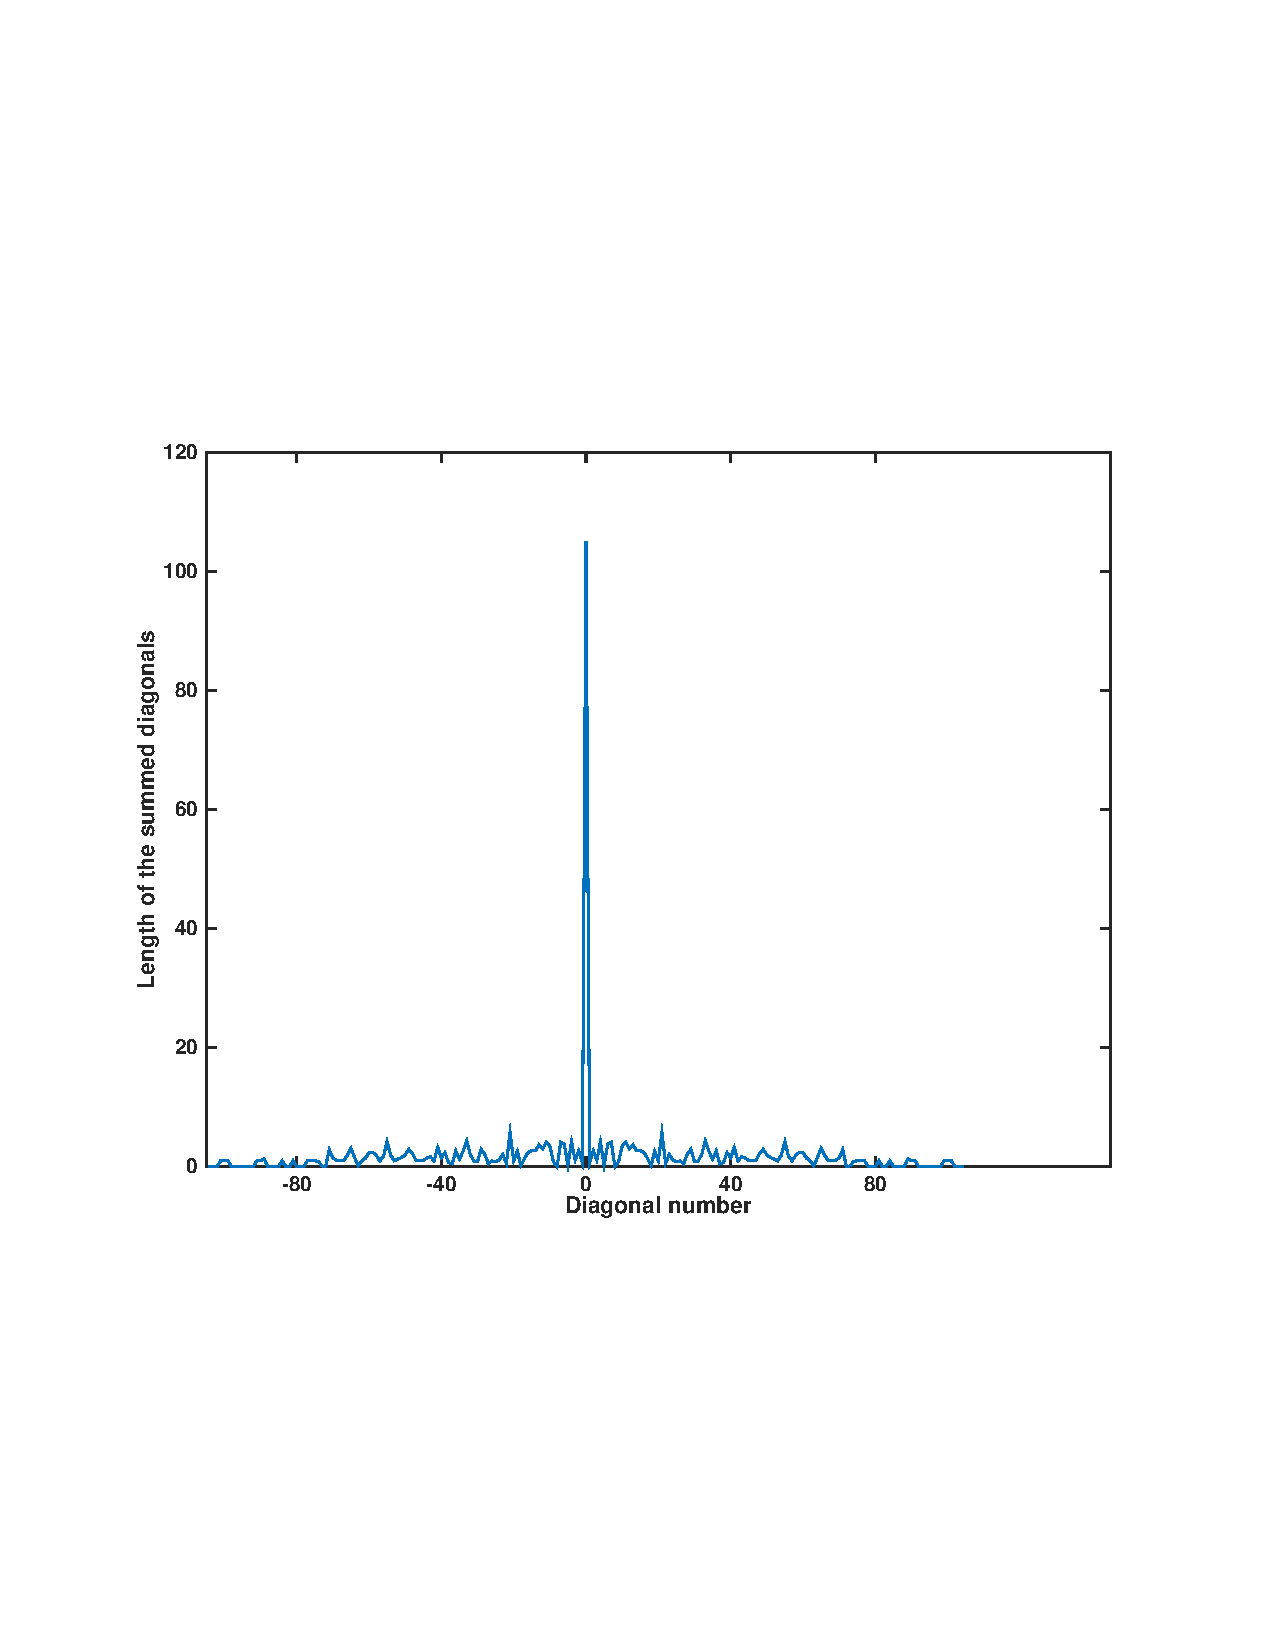
\includegraphics[width=0.6\textwidth]{Plots/diagonal-sums}
	\caption{The sub-diagonal elements, $\mathrm{e}^{-j \omega \Delta t_{kl}}$, of the product $\mathbf{\Gamma \Gamma}^H$ are summed. The length of each output is plotted. The spike is caused by the main diagonal elements of $\mathbf{\Gamma \Gamma}^H$ because they are all in phase.}
	\label{fig:Ch-Results-Diagonal-Sums}
\end{figure}

The closer Figure \ref{fig:Ch-Results-Diagonal-Sums} comes to a spike the more incoherent is the blending pattern. Thus, considering Figure \ref{fig:Ch-Results-Diagonal-Sums} the incoherency, $\mu$, is measured as the ratio between the amplitude of the spike and the sum of all amplitudes. 

In terms of the sub-diagonals of $\mathbf{\Gamma \Gamma}^H$ this is the ratio between the squared absolute value of the summed main diagonal and the sum of all squared absolute summed sub-diagonals;

\begin{equation}
	\mu(\omega) = \frac{  \left| \sum_{j-i = 0} \mathbf{\Gamma \Gamma}^H_{ij} (\omega) \right|^2    }{ \sum_{k = 1-N_s}^{N_s-1}	 \left( \left| \sum_{j-i = k} \mathbf{\Gamma \Gamma}^H_{ij} (\omega) \right|^2 \right)   }.
	\label{eq:Ch-Results-incoherency-monochromatic}
\end{equation}

Note that $N_s$ is the number of sources, i.e. the matrix $\mathbf{\Gamma \Gamma}^H$ has $N_s$ rows and columns.

Up to now, the incoherency is computed for each frequency separately. In order to account for all frequencies at once the nominator and denominator in equation \ref{eq:Ch-Results-incoherency-monochromatic} are summed over all frequency components;

\begin{equation}
	\mu = \frac{  \sum_{\omega} \left( \left| \sum_{j-i = 0} \mathbf{\Gamma \Gamma}^H_{ij} (\omega) \right|^2  \right)  }{  \sum_{\omega} \left( \sum_{k = 1-N_s}^{N_s-1}	 \left( \left| \sum_{j-i = k} \mathbf{\Gamma \Gamma}^H_{ij} (\omega) \right|^2 \right) \right)  } \;.
	\label{eq:Ch-Results-incoherency2}
\end{equation}



For example, for a perfectly incoherent blending pattern only the sum along the main diagonal ($k=0$) is non zero. Thus, the nominator and the denominator in equation \ref{eq:Ch-Results-incoherency} are identical, the incoherency equals 1. 

In contrast, for a perfectly coherent blending pattern all sub-diagonal elements are in phase. Consequently, the sum along the main diagonal is of the same magnitude as the sum along the sub-diagonals. The nominator in equation \ref{eq:Ch-Results-incoherency} becomes significantly smaller than the denominator, and the incoherency is nearly 0.


\section{Results}

\section{Effect of Maximum Firing Time Delay}

\section{Results}



    	\chapter{Crossline Deblending (3D)} \label{chap:MahdadMethod3d}

This thesis proposes to blend crossline sources. It is hypothesized that by combining several cross-lines one can effectively blend sources in 3D.

The deblending method of \citet{Mahdad-Deblending-Method} described in section \ref{sec:MahdadMethod} is designed for 2D blended data. In this chapter I will explain how each step of the Mahdad method can be extended to 3D data, and I will demonstrate its strengths and  performance.

First, the data sorting will be modified such that the blended 3D data can be described using the same forward model as in section \ref{sec:Ch-Theory-Operator}. The presented data sorting will allow to maintain all other steps of the deblending algorithm of \citet{Mahdad-Deblending-Method}. Second, the 2D $f$-$k$ filter will be extended to a 3D $f$-$k_x$-$k_y$ filter to remove noise in both crossline and inline direction.

\section{Data Sorting} \label{sec:Ch-Theory-3dExtension-DataSorting}

\subsection*{Data Matrix}

In 3D acquisition the sources and receivers are distributed on a 2D surface. Thus, their locations are defined by their inline and crossline positions, ($x$, $y$). Each data point which is measured by a source receiver pair at a specific time is therefore described by 5 coordinates, time $t$, receiver inline and crossline position ($x_r$, $y_r$), and source inline and crossline position ($x_s$, $y_s$).

Similar as in section \ref{sec:Ch-Theory-Operator} the 5D data "cube" will be again reorganized in a 2D data matrix according to \citet{Delphi-Format} (see Figure \ref{fig:Ch-Theory-DelphiFormat}). For this data sorting a 1D Fourier transform with respect to time is performed and a 4D frequency "slice" is selected.

The 4D "slice" is sorted in a 2D data matrix, $\mathbf{P}$, with as many rows as receivers and as many columns as shots. The total number of shots is obtained by multiplying the number of shots fired in each crossline and the number of shots fired in each inline. The total number of receivers is obtained likewise. Assume there are $Ns_x$ shots per crossline. The shots of the first crossline are assigned to the first $Ns_x$ columns of the data matrix, the shots of the second crossline are assigned to the next $Ns_x$ columns of the data matrix, etc. The receivers are sorted in the rows of the data matrix analogously.

\nomenclature{$Ns_x$}{Number of sources in crossline direction}
\nomenclature{$Ns_y$}{Number of sources in inline direction}
\nomenclature{$x$}{Crossline space coordinate}
\nomenclature{$y$}{Inline space coordinate}
\nomenclature{CRG}{Common-receiver gather}
\nomenclature{CSG}{Common-shot gather}

One row in the data matrix, $\mathbf{P}$, in Figure \ref{fig:Ch-Theory-DelphiFormat} represents  a 3D common-receiver gather. The data of this 3D common-receiver gather are shown in Figure \ref{fig:Ch-Theory-Data3d} in a 3D view, where the coordinates, $x$ and $y$, indicate the inline and crossline shot position respectively. For the described data sorting individual crossline slices are extracted from this data cube and assembled next to each other in a data matrix as shown in Figure \ref{fig:Ch-Theory-Data3d_Delphi}. This view will be referred to as 3D CRG 2D view. Each hyperbolic event refers to the response of the shots of one crossline.

\begin{figure}
	\centering
	\includegraphics[width=0.6\textwidth]{Plots/DelphiFormat-v3}
	\caption{Illustration of the data matrix $\mathbf{P}$ for 3D data \citep{Delphi-Format}. $y_r$ and $y_s$ represent the inline receiver and shot positions. $x_r$ and $x_s$ represent the crossline receiver and shot positions. Each row refers to a 3D common-receiver gather and each column to a 3D common-shot gather. A sub-matrix with fixed receiver and source inline positions ($y_r$, $y_s$) is equivalent to a data matrix for 2D acquisition.}
	\label{fig:Ch-Theory-DelphiFormat}
\end{figure}


\begin{figure}
	
	\begin{subfigure}[t]{\textwidth}
	 	\centering
		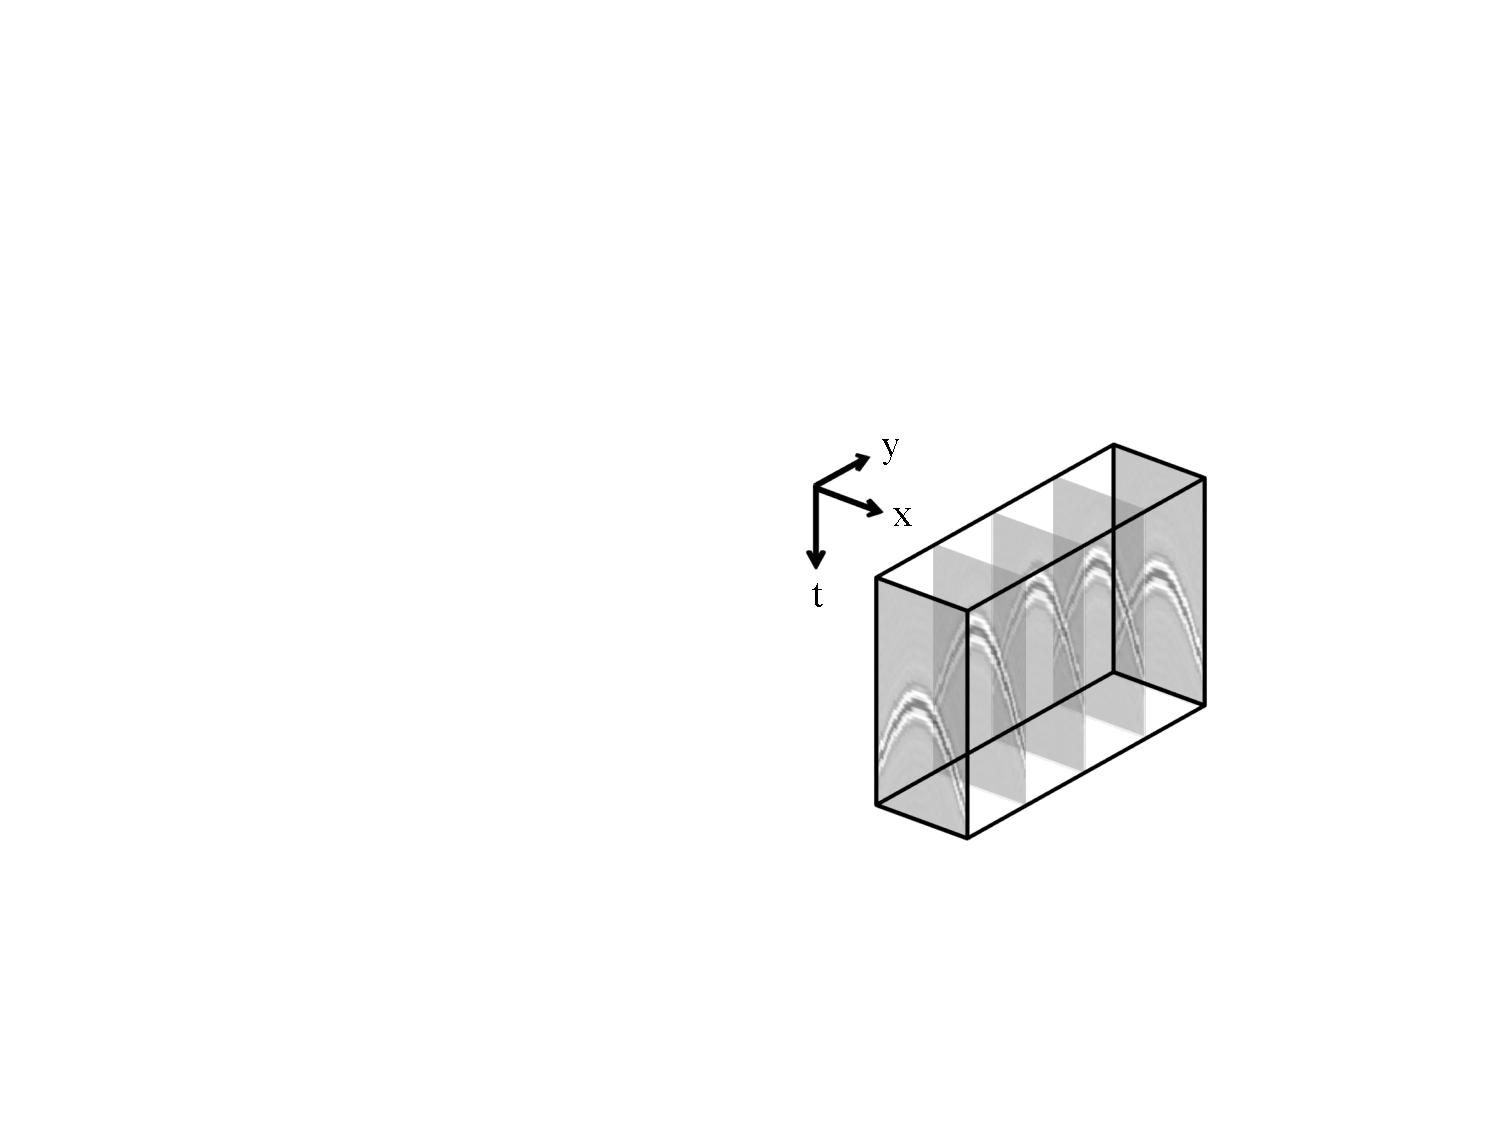
\includegraphics[width = 0.3\textwidth]{Plots/data3d}
		\caption{}
		\label{fig:Ch-Theory-Data3d}
	\end{subfigure}
	\par\bigskip
	\begin{subfigure}[t]{\textwidth}
		\centering
		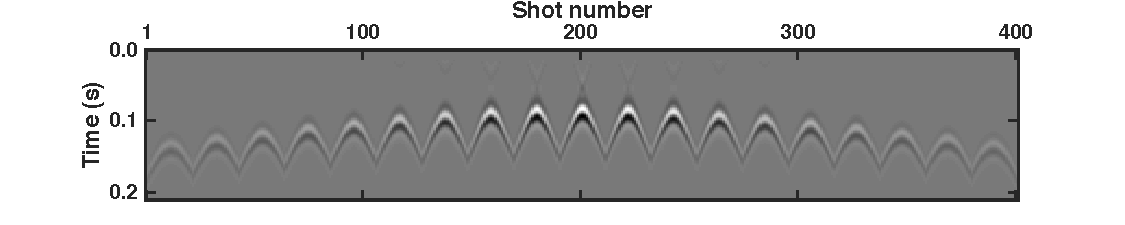
\includegraphics[width = \textwidth]{Plots/IdealData3d/p_Delphi}
		\caption{}
		\label{fig:Ch-Theory-Data3d_Delphi}
	\end{subfigure}
	
	\caption{(a) 3D common-receiver gather with crossline (x) and inline (y) sources (3D view). (b) Resorted data set. Individual crossline sections are plotted next to each other in 2D. For visibility both subfigures only show a reduced part of the data. This view is called 3D CRG 2D view.}
	\label{fig:Ch-Theory-DataSorting}
\end{figure}


\subsection*{Blending matrix}

The blending matrix for 3D is built in a similar fashion as the data matrix in 3D. As described in section \ref{sec:BlendingMatrix} each row of the blending matrix, $\mathbf{\Gamma}$, captures one shot. For extension to 3D the shots of the first crossline are placed in the top $Ns_x$ rows of the blending matrix, followed by the shots of the second crossline etc. (see Figure \ref{fig:Ch-Theory-3D-BlendingMatrix-Design}). The elements in the $j^{th}$ column of the blending matrix, $\mathbf{\Gamma}$, select the shots which are blended in the $j^{th}$ experiment. For example, the first column of the blending matrix in Figure \ref{fig:Ch-Theory-3D-BlendingMatrix} describes that in the first experiment shots (rows) $1$ and $3$ are blended with a time delay of $\Delta t_1$.

\todo[inline]{Keep this sentence for later: This framework allows to blend any source combination independent of the cross- and inline positions of the involved sources.}

With the new data and blending matrix sorting one can apply deblending to 3D data in the same way as presented in section \ref{sec:Ch-Theory-Operator} and section \ref{sec:MahdadMethod}. Note that unlike for 2D blending spatially incoherent blending patterns are practical for 3D blended acquisition.

\begin{figure}

	\begin{subfigure}[t]{0.5\textwidth}
		\centering
		\includegraphics[width = \textwidth]{Plots/DrawingsCartesianFormat3}
		\caption{}
		\label{fig:Ch-Theory-3D-BlendedAcquisition}
	\end{subfigure}
	%
	\begin{subfigure}[t]{0.5\textwidth}
		\centering
		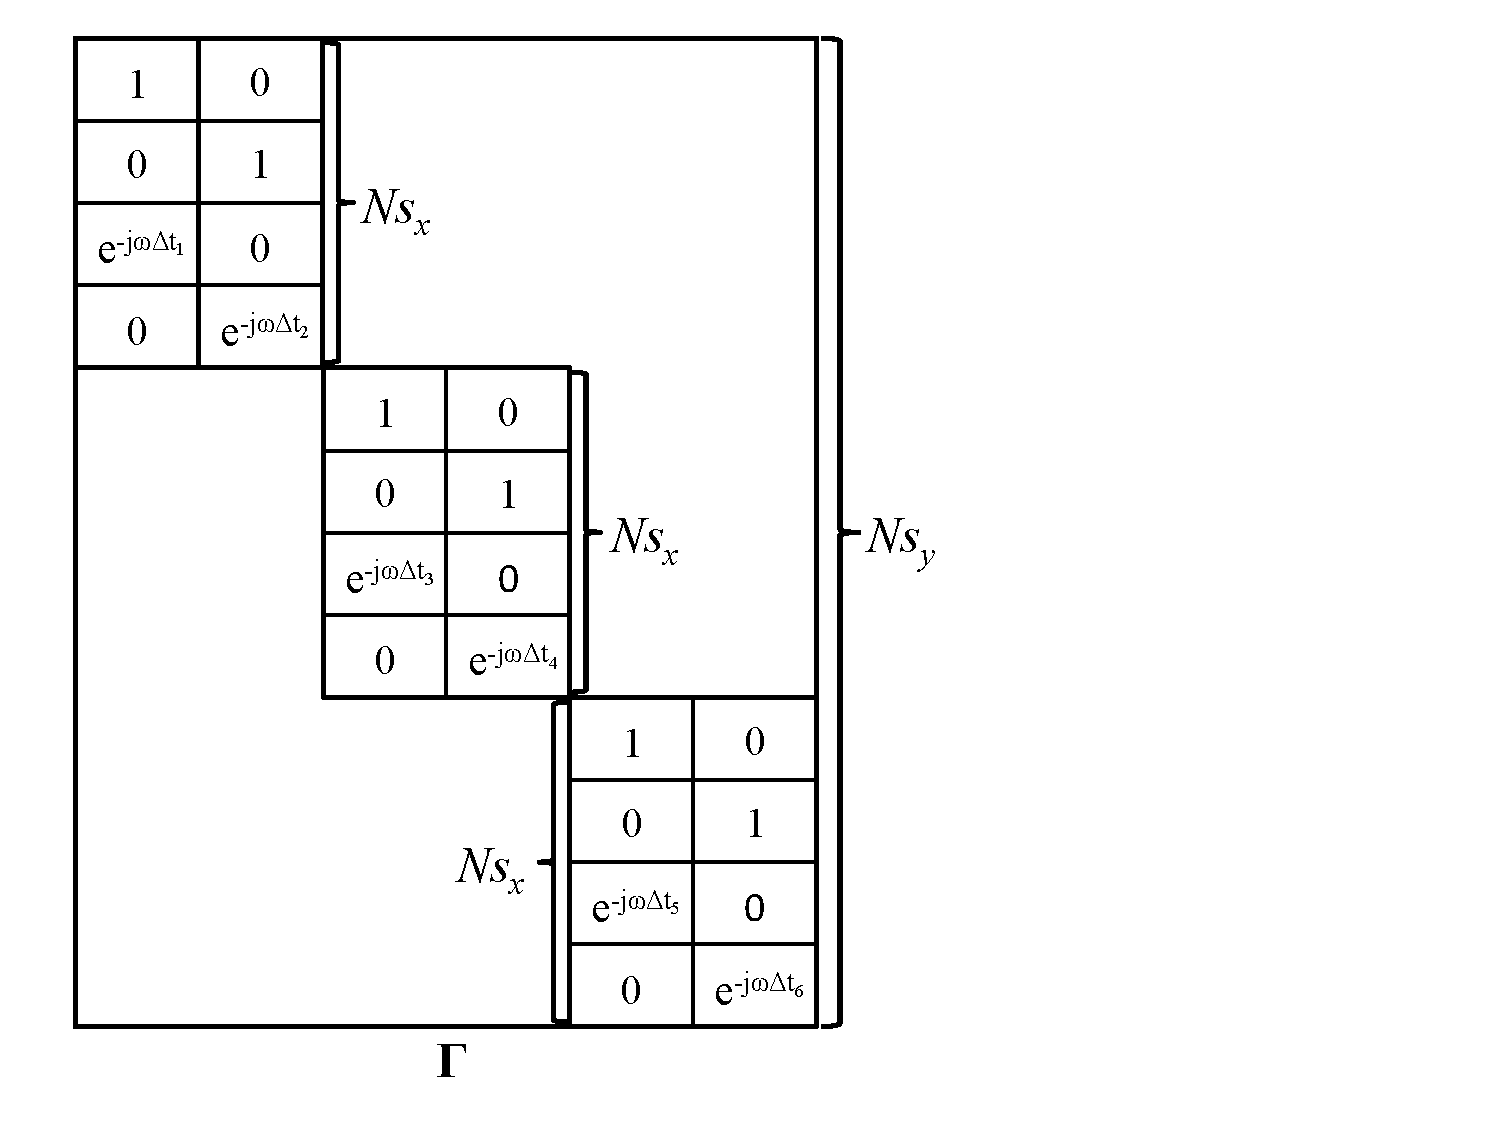
\includegraphics[width = 0.7\textwidth]{Plots/DrawingsCartesianFormat2}
		\caption{}
		\label{fig:Ch-Theory-3D-BlendingMatrix}
	\end{subfigure}
	
	\caption{Illustration of the blending matrix, $\mathbf{\Gamma}$, for 3D acquisition. (a) At each of the $Ns_y$ inline position the crossline sources ($x$ direction) are blended. Each of these 2D blending processes is described by a 2D blending matrix, which has as many rows as there are crossline sources, $Ns_x$. (b) The 2D blending matrices are assembled in a single 3D blending matrix, $\mathbf{\Gamma}$, which has $Ns_x$ by $Ns_y$ rows.}
	\label{fig:Ch-Theory-3D-BlendingMatrix-Design}

\end{figure}


\section{3D $f$-$k_x$-$k_y$ Filter} \label{sec:Ch-Theory-3dExtension-FKK}

In section \ref{sec:IterBlenNoiseEst} the 2D $f$-$k$ filter was introduced. In 3D there are two spatial directions ($x$,$y$), i.e. the filter can be extended to a 3D $f$-$k_x$-$k_y$ filter.

For this purpose one considers a 3D common-receiver gather, $\mathbf{p}(t,x_s,y_s)$, and brings it to the $f$-$k_x$-$k_y$ domain by applying a 3-dimensional Fourier transform. Next, a constant frequency slice is selected. This leaves a 2D matrix, which captures the crossline and inline wavenumbers ($k_x$, $k_y$) as shown in Figure \ref{fig:Ch-Theory-FK-f_slice-data}. The minimum wavefield velocity, $v_{min}$, and the frequency, $f$, determine the maximum wavenumber, $k_{max}$, according to equation \ref{eq_Ch-Theory-MaxWavenmber};

\begin{equation}
	k_{max} = \frac{f}{v_{min}}.
	\label{eq_Ch-Theory-MaxWavenmber-Repetition}
\end{equation} 

The total wavenumber, $k_{T}$, must be smaller than the maximum wavenumber, $k_{max}$,

\begin{equation}
	k_{T} = \sqrt{k_x^2 + k_{y}^2} < k_{max}.
	\label{eq:Ch-Theory-TotalWavenumber}
\end{equation}
\nomenclature{$k_T$}{Total wavenumber}

Hence the signal "cone" is defined by a circle (see Figure \ref{fig:Ch-Theory-FK-f_slice-mask}). This is repeated for each frequency component, such that the overall $f$-$k_x$-$k_y$ mask is a 3D cone (see Figure \ref{fig:Ch-Theory-FK-f_slice-data3d}). The cone can be sorted in a 2D view according to section \ref{sec:Ch-Theory-3dExtension-DataSorting} as illustrated in Figure \ref{fig:Ch-Theory-FK-delphi-data} and Figure \ref{fig:Ch-Theory-FK-delphi-mask}. Finally, this mask is computed for each receiver gather.

For comparison, a 2D $f$-$k$ filter is designed for 3D data and plotted in a 2D view in Figure \ref{fig:Ch-Mahdad3d-2dfk}. Note that the 3D $f$-$k_x$-$k_y$ filter (see Figure \ref{fig:Ch-Theory-FKK-Mask}) removes significantly more incoherent energy than the 2D $f$-$k$ filter. 

%The maximum crossline wavenumber, $k_x$, is defined according to section \ref{sec:IterBlenNoiseEst}. The resulting $f$-$k$-mask is shown in Figure \ref{fig:Ch-Mahdad3d-2dfk}. Note that it only filters the crossline wavenumbers $k_x$, i.e. it is a $f$-$k_x$ filter.

%The $f$-$k_x$-$k_y$ spectra of synthetic data shown in Figure \ref{fig:Ch-Theory-FK-f_slice-data} and \ref{fig:Ch-Theory-FK-delphi-data} illustrate that the 2D $f$-$k_x$-filter will also pass some energy which is not signal. In the following both spatial directions, $x$ and $y$, are considered to extend the filter to a 3D $f$-$k_x$-$k_y$-filter.

\begin{figure}
	\centering
	\begin{subfigure}[t]{0.3\textwidth}
		\centering
		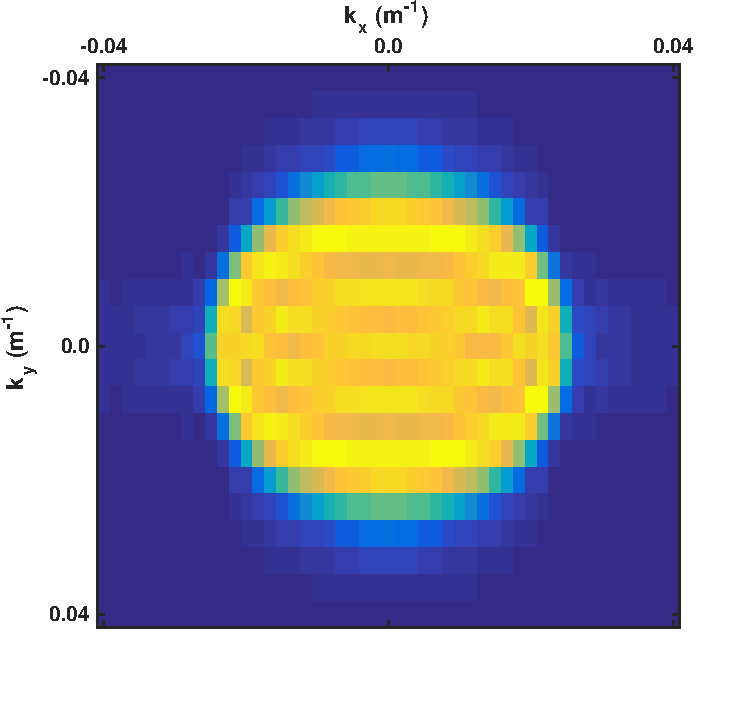
\includegraphics[width=\textwidth]{Plots/IdealData3d/P_f_slice40}
		\caption{}
		\label{fig:Ch-Theory-FK-f_slice-data}
	\end{subfigure}
	%
	\centering
	\begin{subfigure}[t]{0.3\textwidth}
		\centering
		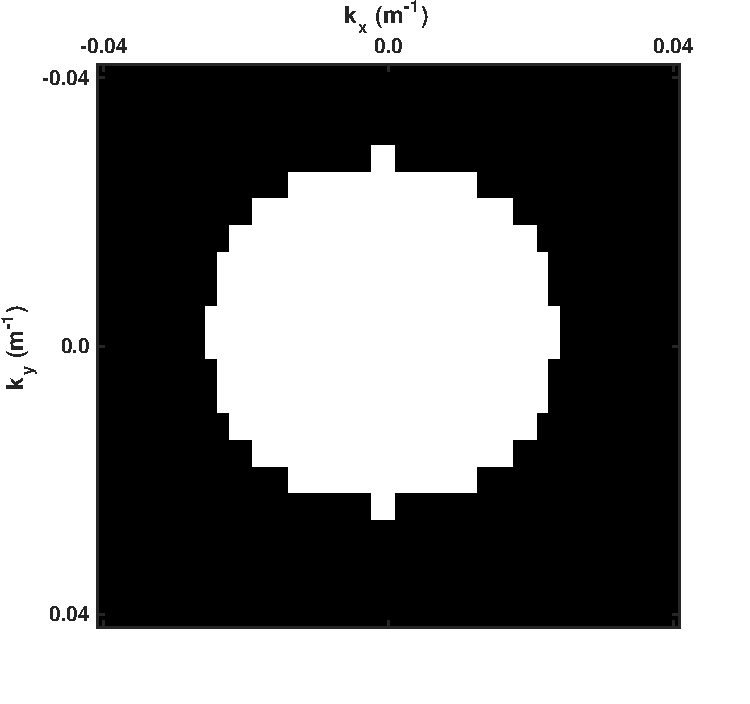
\includegraphics[width=\textwidth]{Plots/IdealData3d/fkk-mask-slice40}
		\caption{}
		\label{fig:Ch-Theory-FK-f_slice-mask}
	\end{subfigure}
	%
	\centering
	\begin{subfigure}[t]{0.3\textwidth}
		\centering
		\includegraphics[width=\textwidth]{Plots/IdealData3d/fk-slices/3dfk-cone}
		\caption{}
		\label{fig:Ch-Theory-FK-f_slice-data3d}
	\end{subfigure}
	
	\begin{subfigure}[t]{\textwidth}
		\centering
		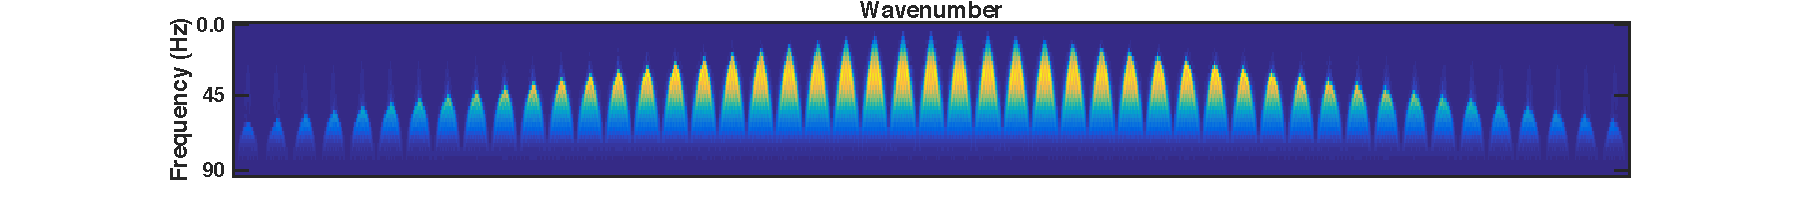
\includegraphics[width=0.9\textwidth]{Plots/IdealData3d/P_fkk_Delphi}
		\caption{}
		\label{fig:Ch-Theory-FK-delphi-data}
	\end{subfigure}
	\par\bigskip
	\begin{subfigure}[t]{\textwidth}
		\centering
		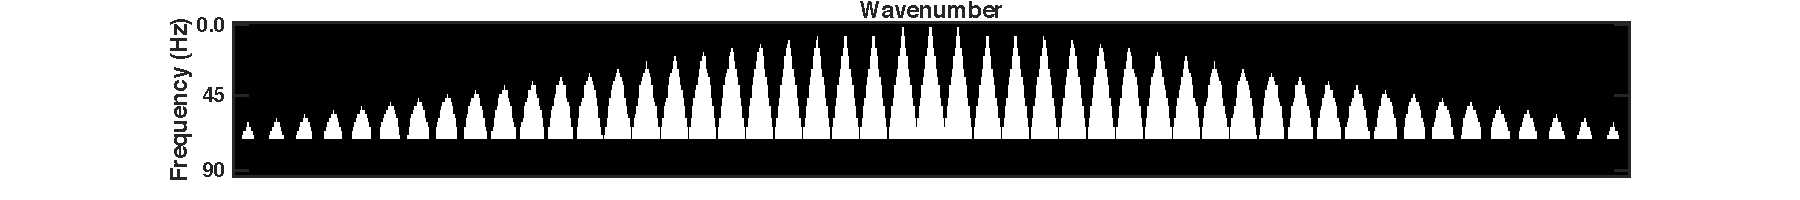
\includegraphics[width=0.9\textwidth]{Plots/IdealData3d/fkk-mask-Delphi}
		\caption{}
		\label{fig:Ch-Theory-FK-delphi-mask}
	\end{subfigure}
	
	\caption{Illustration of the 3D $f$-$k_x$-$k_y$ filter. (a) is a \SI{40}{\hertz} frequency slice of the $f$-$k_x$-$k_y$ spectrum of the data in Figure \ref{fig:Ch-Theory-DataSorting}. $k_x$ and $k_y$ refer to the crossline and inline wavenumber respectively. (b) is a \SI{40}{\hertz} frequency slice of the $f$-$k_x$-$k_y$ mask, where the white area equals 1 and the black area is 0. (c) shows the \SI{40}{\hertz} frequency slice of (a) sorted in a 3D cube. The red cone represents the edge of the 3D $f$-$k_x$-$k_y$ filter mask. (d) and (e) display the $f$-$k_x$-$k_y$ data spectrum and mask sorted according to section \ref{sec:Ch-Theory-3dExtension-DataSorting}, i.e. each sub-cone refers to one inline wavenumber. Note that due to the sorting the wavenumber axis is a mix of crossline and inline wavenumbers. For this reason the wavenumber axis has no labels.}
	\label{fig:Ch-Theory-FKK-Mask}

\end{figure}



\begin{figure}

	\centering 
	\begin{subfigure}[t]{0.45\textwidth}
		\centering
		\includegraphics[width = 0.65\textwidth]{Plots/IdealData3d/fkk-mask-slice40-2d}
		\caption{}
		\label{fig:Ch-Mahdad3d-2dfk-slice}
	\end{subfigure}
	
	\par\bigskip
	
	\centering
	\begin{subfigure}[t]{\textwidth}
		\centering
		\includegraphics[width = 0.9\textwidth]{Plots/IdealData3d/fkk-mask-Delphi-2d}
		\caption{}
		\label{fig:Ch-Mahdad3d-2dfk-Delphi}
	\end{subfigure}
	
	\caption{2D $f$-$k_x$ filter for 3D data. (a) shows a \SI{40}{\hertz} frequency slice of the $f$-$k_x$-$k_y$ spectrum, where the white area equals 1 and the black area is 0. Note that the filter is not affecting the inline wavenumbers $k_y$. (b) illustrates the 2D $f$-$k_x$ filter sorted according to section \ref{sec:Ch-Theory-3dExtension-DataSorting}. Each cone represents a 2D $f$-$k$ filter for a single inline wavenumber.}
	\label{fig:Ch-Mahdad3d-2dfk}
\end{figure}



\begin{comment}
Once the mask is built for a 5D data array it can either be applied to filter a 5D data array, or the mask is sorted to 2D according to section \ref{sec:Ch-Theory-3dExtension-DataSorting}, and applied to the $f$-$k_x$-$k_y$-spectrum of the data matrix (see Figure \ref{fig:Ch-Theory-FK-delphi-data}, \ref{fig:Ch-Theory-FK-delphi-mask}).
\end{comment}




\section{Results}

The 3D $f$-$k_x$-$k_y$ filter removes incoherent energy in the crossline and inline direction. The 3D blended acquisition design suggested in this thesis blends shots within the same crossline. Hence, an underlying question is whether an extension of the 2D $f$-$k_x$ filter to the inline direction provides significant deblending enhancements.

For this purpose the synthetic data of Figure \ref{fig:Ch-Mahdad3d-Unbl-Delphi} are blended: Within each crossline there are 21 sources, which are blended in 3 experiments. For each experiment 7 randomly selected sources are blended with random time delays, i.e. the blending pattern with mixed incoherency is applied. The maximum allowed firing-time delay is set to \SI{400}{\milli\second}. The incoherency measure of the used blending matrix, $\mathbf{\Gamma}$, is $\mu = \SI{99}{\percent}$. 

The blended data are deblended with the 3D deblending algorithm. In one case a 2D $f$-$k_x$ filter is applied (see Figure \ref{fig:Ch-Mahdad3d-Deblending-2dfk}). In the other case a 3D $f$-$k_x$-$k_y$ filter is applied (see Figure \ref{fig:Ch-Mahdad3d-Deblending-3dfk}). It is clearly visible that the deblending quality increases significantly with the 3D $f$-$k_x$-$k_y$ filter. Figure \ref{fig:Ch-Mahdad3d-Deblending-2dvs3d-fk-tslice} displays a $\SI{420}{\milli\second}$ time slice of each subplot in Figure \ref{fig:Ch-Mahdad3d-Deblending-2dvs3d-fk}.
 
\begin{figure}
	
	\centering
	\begin{subfigure}[t]{0.8\textwidth}
		\centering
		\includegraphics[width = \textwidth]{Plots/BlendingPatterns/Unblended_Delphi_zoom-font14}
		\caption{Unblended synthetic data}
		\label{fig:Ch-Mahdad3d-Unbl-Delphi}
	\end{subfigure}

	\par\bigskip
	
	\centering
	\begin{subfigure}[t]{0.8\textwidth}
		\includegraphics[width = \textwidth]{Plots/BlendingPatterns/Pseudo-Deblendedv5_xt_100}
		\caption{Pseudo-deblended data}
		\label{fig:Ch-Mahdad3d-Deblending-Pseudo-Zoom}
	\end{subfigure}
	
	\par\bigskip

	\centering
	\begin{subfigure}[t]{0.8\textwidth}
		\includegraphics[width = \textwidth]{Plots/2dvs3dfk/Deblendedv6_xt_100}
		\caption{Deblended data with a 2D $f$-$k_x$ filter}
		\label{fig:Ch-Mahdad3d-Deblending-2dfk}
	\end{subfigure}
	
	\par\bigskip
	
	\centering
	\begin{subfigure}[t]{0.8\textwidth}
		\includegraphics[width = \textwidth]{Plots/2dvs3dfk/Deblendedv5_xt_100}
		\caption{Deblended data with a 3D $f$-$k_x$-$k_y$ filter}
		\label{fig:Ch-Mahdad3d-Deblending-3dfk}
	\end{subfigure}
	
	\caption{(a) is a synthetic 3D common-receiver gather in 2D view. The data are generated by 21 crossline shots and 51 inline shots. The shown section is a zoom on the strongest events. Figure \ref{fig:Ch-Results-Unbl-inline10} shows one crossline of the data for all times. The data are blended with a mixed incoherency blending pattern. Then, the 3D deblending algorithm is applied. (b) shows the pseudo-deblended data. In case (c) the algorithm uses a 2D $f$-$k_x$ filter. In case (d) it uses a 3D $f$-$k_x$-$k_y$ filter.}
	\label{fig:Ch-Mahdad3d-Deblending-2dvs3d-fk}
	
\end{figure}


\begin{figure}
	
	\centering
	\begin{subfigure}[t]{0.45\textwidth}
		\centering
		\includegraphics[width = \textwidth]{Plots/BlendingPatterns/time-slices/Unblendedv5_100-tslice}
		\caption{Unblended synthetic data}
		\label{fig:Ch-Mahdad3d-Unbl-Delphi-tslice}
	\end{subfigure}
	%
	\centering
	\begin{subfigure}[t]{0.45\textwidth}
		\includegraphics[width = \textwidth]{Plots/BlendingPatterns/time-slices/Pseudo-Deblendedv5_xt_100-tslice_b7}
		\caption{Pseudo-deblended data}
		\label{fig:Ch-Mahdad3d-Deblending-Pseudo-Zoom-tslice}
	\end{subfigure}
	
	\par\bigskip

	\centering
	\begin{subfigure}[t]{0.45\textwidth}
		\includegraphics[width = \textwidth]{Plots/BlendingPatterns/time-slices/Deblendedv6_xt_100-tslice}
		\caption{Deblended data with a 2D $f$-$k_x$ filter}
		\label{fig:Ch-Mahdad3d-Deblending-2dfk-tslice}
	\end{subfigure}
	%
	\centering
	\begin{subfigure}[t]{0.45\textwidth}
		\includegraphics[width = \textwidth]{Plots/BlendingPatterns/time-slices/Deblendedv5_xt_100-tslice}
		\caption{Deblended data with a 3D $f$-$k_x$-$k_y$ filter}
		\label{fig:Ch-Mahdad3d-Deblending-3dfk-tslice}
	\end{subfigure}
	
	\caption{(a) - (d) show \SI{420}{\milli\second} time slices of the data in Figure \ref{fig:Ch-Mahdad3d-Deblending-2dvs3d-fk}.}
	\label{fig:Ch-Mahdad3d-Deblending-2dvs3d-fk-tslice}
	
\end{figure}


In order to quantify the quality gap between the results with 2D and 3D filters, the data of Figure \ref{fig:Ch-Mahdad3d-Unbl-Delphi} are blended with maximum firing-time delays varying between \SI{40}{\milli\second} and \SI{400}{\milli\second}. The blended data are deblended in one case with a 2D $f$-$k$ filter, and in the other case with a 3D $f$-$k_x$-$k_y$ filter. The resulting quality factors are shown in Figure \ref{fig:Ch-Mahdad3d-2dvs3dfk}.



\begin{figure}
	\centering
	\includegraphics[width = 0.6\textwidth]{Plots/2dvs3dfk/Q_2d-vs-3d_fk_v2}
	\caption{Comparison of the deblending quality with a 2D $f$-$k_x$ filter and a 3D $f$-$k_x$-$k_y$ filter. The data in Figure \ref{fig:Ch-Mahdad3d-Unbl-Delphi} are blended with varying maximum firing-time delay. Then the blended data are deblended using a 2D $f$-$k_x$ filter and a 3D $f$-$k_x$-$k_y$ filter.}
	\label{fig:Ch-Mahdad3d-2dvs3dfk}
\end{figure}

\FloatBarrier


\section{Conclusions}

The presented deblending method uses a coherency constraint. It has been demonstrated that for 3D deblending the quality of the deblended data can be enhanced significantly by extending the coherency constraint to crossline direction too.



















    	\include{Chapters/chapter-ComplexData}
    	\include{Chapters/chapter-DiscussionConclusion}
    	%\chapter{Results}

This chapter presents the major results of this thesis. First, an optimal blending pattern for simultaneous crossline sources will be derived. Then, the advantages of a 3D $f$-$k_x$-$k_y$-filter towards a 2D $f$-$k$-filter will be shown. Finally, the feasibility of the suggested acquisition design will be proven on a synthetic 3D data set. 

 
\section{Blending pattern}


\begin{itemize}
	\item Explain how the acquisition limits the firing pattern
	\item Introduce spatial incoherency
	\item Suggest the applied blending pattern
	\item Show quality factor versus incoherency/firing pattern
\end{itemize}

An incoherent blending pattern is crucial for good deblending performance (see section \ref{sec:BlendingMatrix}). Thus, a measure of incoherency will be introduced. Then, the importance of the maximum firing delay time will be demonstrated.

\subsection*{Incoherency Measure}

In this thesis only the incoherency of the acquisition design is considered. Thus, the blending matrix, $\Gamma$, determines the incoherency. In section \ref{sec:BlendingMatrix} it was shown that for an incoherent blending pattern the elements, $\mathrm{e}^{-j \omega \Delta t_{kl}}$, along a sub-diagonal of the product $\mathbf{\Gamma \Gamma}^H$ should be out of phase. 

These sub-diagonal elements, $\mathrm{e}^{-j \omega \Delta t_{kl}}$, are complex numbers with unit length and variable phase. Hence, the elements are located in the complex plane on a circle with radius 1 (see Figure \ref{fig:Ch-Results-complex-circle}). 

\begin{figure}
	\centering
	\includegraphics[width = 0.5\textwidth]{Plots/complex-circle}
	\caption{Illustration of the sub-diagonal elements in the complex number plane. The elements have unit length and variable phase. The absolute value of their sum depends on the phase coherency of the elements.}
	\label{fig:Ch-Results-complex-circle}
\end{figure}


If all elements are in phase the length of their sum is maximized. The more the elements are out of phase, i.e. the more incoherent they are, the smaller is the length of the summed elements. Figure \ref{fig:Ch-Results-Diagonal-Sums} illustrates the length of the summed sub-diagonals. The elements on the main diagonal of the product $\mathbf{\Gamma \Gamma}^H$ are all equal to 1. Thus, the spike in Figure \ref{fig:Ch-Results-Diagonal-Sums} refers to the main diagonal of $\mathbf{\Gamma \Gamma}^H$. For a perfectly incoherent blending design the elements on a sub-diagonal cancel and the plot becomes a perfect spike. 


\begin{figure}
	\centering
	\includegraphics[width=0.6\textwidth]{Plots/diagonal-sums}
	\caption{The sub-diagonal elements, $\mathrm{e}^{-j \omega \Delta t_{kl}}$, of the product $\mathbf{\Gamma \Gamma}^H$ are summed. The length of each output is plotted as a function of the diagonal. The spike is caused by the main diagonal elements of $\mathbf{\Gamma \Gamma}^H$ because they are all in phase.}
	\label{fig:Ch-Results-Diagonal-Sums}
\end{figure}

The incoherency, $\mu$, can be quantified by comparing the length of the summed main diagonal of $\mathbf{\Gamma \Gamma}^H$ with the length of the summed sub-diagonals;

\begin{equation}
	\mu = \frac{  \sum_{\omega} \left( \left| \sum \mathbf{\Gamma \Gamma}^H_{00} (\omega) \right|^2  \right)  }{  \sum_{\omega} \left( \sum_{i = 1-N_s}^{N_s-1}	 \left( \left| \sum \mathbf{\Gamma \Gamma}^H_{ii} (\omega) \right|^2 \right) \right)  }
	.
\end{equation}










Different incoherent blending patterns will be tested, in particular, temporally and spatially incoherent blending patterns. 

This thesis considers the following blended acquisition set up: The sources are assembled in crossline direction and move in inline direction due to the vessel movement (see Figure \ref{fig:Ch-Theory-3D-BlendedAcquisition}). As a consequence each experiment can blend sources which belong to the same crossline. The source sampling rate in inline direction must be sufficiently small to avoid spatial aliasing. Thus, the sources within one crossline must be blended and recorded before the vessel reaches the next inline position.

Based on this set up there are three possibilities to blend the sources incoherently. First, the sources can be blended with random time delays (temporal incoherency). Second, one can randomly pick sources for each experiment (spatial incoherency). Third, temporal and spatial incoherency can be combined, i.e. randomly picked sources are blended with random time delays.

In the following these blending patterns will applied to a synthetic data set (see Figure \ref{fig:Ch-Results-Unbl-Delphi}, \ref{fig:Ch-Results-Unbl-inline10}, \ref{fig:Ch-Results-Unbl-xline10}). Next, the data is deblended with the 3D deblending algorithm of section \ref{sec:MahdadMethod3d}. 

The deblending results are shown in Figure \ref{fig:Ch-Results-Debl-Delphi} and \ref{fig:Ch-Results-Debl-x-inline}. The results suggest that only spatial incoherency is not sufficient to deblend the data (see Figure \ref{fig:Ch-Results-Debl-Delphi-x}, \ref{fig:Ch-Results-Debl-inline10-x}, \ref{fig:Ch-Results-Debl-xline10-x}). By introducing random firing time delays the deblended data improves significantly as shown in Figure \ref{fig:Ch-Results-Debl-Delphi-t}, \ref{fig:Ch-Results-Debl-inline10-t}, \ref{fig:Ch-Results-Debl-xline10-t}). A combination of both spatial and temporal incoherency enhances the deblended data further (see Figure \ref{fig:Ch-Results-Debl-Delphi-xt}, \ref{fig:Ch-Results-Debl-inline10-xt}, \ref{fig:Ch-Results-Debl-xline10-xt}).

\begin{figure}
	\centering
	\begin{subfigure}[t]{0.8\textwidth}
		\centering
		\includegraphics[width = \textwidth]{Plots/BlendingPatterns/Unblended_Delphi_zoom}
		\caption{}
		\label{fig:Ch-Results-Unbl-Delphi}
	\end{subfigure}
	\par\bigskip
	\centering
	\begin{subfigure}[t]{0.8\textwidth}
		\centering
		\includegraphics[width = \textwidth]{Plots/BlendingPatterns/Deblended_Delphi_zoomx}
		\caption{}
		\label{fig:Ch-Results-Debl-Delphi-x}
	\end{subfigure}
	\par\bigskip
	\centering
	\begin{subfigure}[t]{0.8\textwidth}
		\centering
		\includegraphics[width = \textwidth]{Plots/BlendingPatterns/Deblended_Delphi_zoomt}
		\caption{}
		\label{fig:Ch-Results-Debl-Delphi-t}
	\end{subfigure}
	\par\bigskip
	\centering
	\begin{subfigure}[t]{0.8\textwidth}
		\centering
		\includegraphics[width = \textwidth]{Plots/BlendingPatterns/Deblended_Delphi_zoomxt}
		\caption{}
		\label{fig:Ch-Results-Debl-Delphi-xt}
	\end{subfigure}
	
	\caption{These 3D common receiver gathers are sorted according to section \ref{sec:Ch-Theory-3dExtension-DataSorting}. The unblended synthetic data (a) is used to simulate a blended acquisition with 3 experiments per crossline and 7 shots per experiment. The maximum firing time delay is \SI{400}{\milli\second}. The sources are blended in three different patterns: (b) Randomly selected sources are blended without time delay, (c) neighboring sources are blended with random time delays, (d) randomly picked sources are blended with random time delays. Next, the blended data sets are deblended. The corresponding deblending results are illustrated in (b) to (d).}
	\label{fig:Ch-Results-Debl-Delphi}
	
\end{figure}

\todo[inline]{Make a sketch of the set up of the synthetic data.}

\begin{figure}
	\centering
	\begin{subfigure}[t]{0.24\textwidth}
		\centering
		\includegraphics[height = 0.38\textheight]{Plots/BlendingPatterns/Unblended_inline10}
		\caption{}
		\label{fig:Ch-Results-Unbl-inline10}
	\end{subfigure}
	%	
	\centering
	\begin{subfigure}[t]{0.24\textwidth}
		\centering
		\includegraphics[height = 0.38\textheight]{Plots/BlendingPatterns/Deblended_inline10x}
		\caption{}
		\label{fig:Ch-Results-Debl-inline10-x}
	\end{subfigure}
	%
	\centering
	\begin{subfigure}[t]{0.24\textwidth}
		\centering
		\includegraphics[height = 0.38\textheight]{Plots/BlendingPatterns/Deblended_inline10t}
		\caption{}
		\label{fig:Ch-Results-Debl-inline10-t}
	\end{subfigure}
	%
	\centering
	\begin{subfigure}[t]{0.24\textwidth}
		\centering
		\includegraphics[height = 0.38\textheight]{Plots/BlendingPatterns/Deblended_inline10xt}
		\caption{}
		\label{fig:Ch-Results-Debl-inline10-xt}
	\end{subfigure}
	\par\bigskip
	\centering
	\begin{subfigure}[t]{0.24\textwidth}
		\centering
		\includegraphics[height = 0.38\textheight]{Plots/BlendingPatterns/Unblended_xline10}
		\caption{}
		\label{fig:Ch-Results-Unbl-xline10}
	\end{subfigure}
	%	
	\centering
	\begin{subfigure}[t]{0.24\textwidth}
		\centering
		\includegraphics[height = 0.38\textheight]{Plots/BlendingPatterns/Deblended_xline10x}
		\caption{}
		\label{fig:Ch-Results-Debl-xline10-x}
	\end{subfigure}
	%
	\centering
	\begin{subfigure}[t]{0.24\textwidth}
		\centering
		\includegraphics[height = 0.38\textheight]{Plots/BlendingPatterns/Deblended_xline10t}
		\caption{}
		\label{fig:Ch-Results-Debl-xline10-t}
	\end{subfigure}
	%
	\centering
	\begin{subfigure}[t]{0.24\textwidth}
		\centering
		\includegraphics[height = 0.38\textheight]{Plots/BlendingPatterns/Deblended_xline10xt}
		\caption{}
		\label{fig:Ch-Results-Debl-xline10-xt}
	\end{subfigure}
	
	\caption{(a)-(d) show inline slices of the data shown in Figure \ref{fig:Ch-Results-Debl-Delphi}. (e)-(h) display the corresponding crossline slices. }
	\label{fig:Ch-Results-Debl-x-inline}

\end{figure}

The deblending performance is quantified with a quality factor, $Q$, which is defined by \citet{IbrahimQuality} as;

\begin{equation}
	Q = 10 \cdot \frac{\left|\left|\text{Unblended data}\right|\right| _2 ^2}{\left|\left|\text{Unblended data - Deblended data}\right|\right| _2 ^2} .	
\end{equation}

Figure \ref{fig:Ch-Results-QualityFactors} illustrates the quality factor for the 3 blending patterns as a function of the maximum firing time delay. The plot confirms the previous observations: Only spatial incoherency limits the deblended data quality, whereas temporal incoherency allows to achieve significantly better deblending performance. The combination of spatial and temporal incoherency can even enhance the result further.

\begin{figure}
	\centering
	\includegraphics[width = 0.6\textwidth]{Plots/BlendingPatterns/quality_line_plot_avg}
	\caption{The 3 suggested blending patterns are simulated with maximum firing time delays between \SI{40}{\milli\second} and \SI{400}{\milli\second}. The quality factors are computed with respect to the unblended data and illustrated as a function of the maximum firing time.}
	\label{fig:Ch-Results-QualityFactors}
\end{figure}

\FloatBarrier
\section{3D FKK Filter Performance}

\section{Feasibility}









		%\chapter{Incoherency} \label{chap::incoherency}

When multiple sources are applied in one experiment the wavefields of the individual sources overlap. \cite{Mahdad-Deblending-Method} presented a method to separate the overlapping wavefields: A key step is pseudo-deblending, which yields the the desired unblended data superimposed by so called blending noise. This noise is generated by the overlap of the individual sources and can be removed with noise filters. However, if the individual wavefields overlap coherently, the blending noise will also be coherent and cannot be removed. In other words it is crucial to fire the sources incoherently.

In this chapter the incoherency of the source overlap is analyzed by considering three questions: Which factors control the incoherency? How can the incoherency be measured? How can the incoherency be maximized for an optimal deblending result?

\section{Incoherency Control Factors}

The deblended data can be represented by

\begin{equation}
	\mathbf{ P_{debl} } = \mathbf{X S \Gamma \Gamma ^H}.
	\label{eq:Ch-Incoherency-Deblended-Data}
\end{equation} 

Each of the matrices in the above equation influences the degree of incoherency of the source overlap. First, the contribution of the Earth \textbf{X} is neglected because it cannot be controlled in a seismic experiment. Second, the source signature \textbf{S}, in particular its time duration, determines the required minimum time delay between sources to avoid an overlap. Consequently, when designing an acquisition with simultaneous sources one must take into account the source signature. Thirdly, the incoherency is strongly dependent on the blending matrix $\mathbf{\Gamma}$ because it captures the firing pattern, i.e. it knows which sources are superimposed and the time delays between the sources in a given experiment. Therefore, the main focus of the incoherency analysis will be on the blending matrix $\mathbf{\Gamma}$.

\section{Quantification of Incoherency}

A mathematical tool to express incoherency is the autocorrelation function $R(\tau)$,

\begin{equation}
	R(\tau) = \int\limits_{\mathbb{R}} f^*(x) f(x + \tau) \, \text{d} x.
	\label{eq:Ch-Incoherency-Autocorrelation}
\end{equation}

For example, in a 1D case the autocorrelation of a fully incoherent function is a spike at zero lag. If a coherent or repetitive pattern is present in a function the autocorrelation will also have non zero amplitudes at other lags. 

For comparative purposes the incoherency of a function $f(x)$ should be quantified. It is suggested to measure incoherency $\mu$ as the ratio of the squared zero lag autocorrelation and the sum of the squared autocorrelation amplitudes,

\begin{equation}
	\mu = \frac{R(\tau = 0)^2}{\sum\limits_{\tau} R(\tau)^2}	.
	\label{eq:Ch-Incoherency-Incoherency}
\end{equation} 

This expression quantifies incoherency as a number between 0 and 1. A fully incoherent function $f(x)$ yields an autocorrelation which is a perfect spike. Thus, the ratio in equation \ref{eq:Ch-Incoherency-Incoherency} equals 1. For a perfectly coherent function $f(x)$ the ratio in equation \ref{eq:Ch-Incoherency-Incoherency} is nearly zero.

The incoherency strongly depends on the blending matrix $\mathbf{\Gamma}$ which is a 3D array. Before applying an autocorrelation the blending matrix $\mathbf{\Gamma}$ is transformed to time domain. The time domain blending matrix is denoted as $\mathbf{\gamma}$. It has the dimensions

\begin{equation}
	\text{dim}(\mathbf{\gamma}) = \text{Sources x Experiments x Time}.
	\label{eq:Ch-Incoherency-gamma}
\end{equation}

If a source $s_i$ is fired in an experiment $e_i$ at a time $t_i$ the element $(s_i,e_i,t_i)$ of $\mathbf{\gamma}$ is 1, else it is 0. If the source is not a perfect spike its amplitude can smear out across several time samples in the matrix $\mathbf{\gamma}$.

The incoherency of the blending matrix $\mathbf{\gamma}$ can be quantified by replacing the 1D autocorrelation in equation \ref{eq:Ch-Incoherency-Autocorrelation} and \ref{eq:Ch-Incoherency-Incoherency} with a 3D autocorrelation, which can be written as,

\begin{equation}
	R(\tau_1,\tau_2,\tau_3) = \iiint\limits_{\mathbb{R}^3} f^*(x,y,z) f(x + \tau_1,y + \tau_2, z + \tau_3) \, \text{d} x \, \text{d} y \, \text{d} z.
	\label{eq:Ch-Incoherency-3dAutocorrelation}
\end{equation}

\todo[inline]{The calculation of the 3D autocorrelation function requires significant computational power such that symmetry properties of the autocorrelation should be exploited to reduce the cost. Symmetry with respect to the origin, but using convn in Matlab I cannot access it}

The elements of the resulting 3D autocorrelation array are a measure for the correlation between wavefields at a specific source, experiment and time lag. For example, if in each experiment adjacent sources are fired with a constant time delay $\Delta t$, the 3D autocorrelation will yield a high amplitude at the source lag 1, experiment lag 0 and time lag $\Delta t$.

Combining equations \ref{eq:Ch-Incoherency-Incoherency} and \ref{eq:Ch-Incoherency-3dAutocorrelation} the incoherency of the time domain blending matrix $\mathbf{\gamma}$ can be expressed as,

\begin{equation}
	\mu = \frac{R(\tau_1 = 0,\tau_2 = 0,\tau_3 = 0)^2}{\sum\limits_{(\tau_1,\tau_2,\tau_3)} R(\tau_1,\tau_2,\tau_3)^2}	.
	\label{eq:Ch-Incoherency-Incoherency3d}
\end{equation} 

\section{Optimization of Incoherency}

\todo[inline]{Relate the incoherency estimate to the quality factor of the deblending. Point out that the quality factor is very sensitive to the time incoherency while the incoherency with respect to experiments or sources has less impact on the deblending performance.}

\section{Fingerprint of the Incoherency in the Blending Matrix $\mathbf{\Gamma}$}

To achieve a better understanding of the blending process the relation between the incoherency quantification and the blending matrix $\Gamma$ is assessed.

In frequency domain the blending matrix has the dimension,

\begin{equation}
	\text{dim}(\mathbf{\Gamma}) = \text{Sources x Experiments x Frequency},
	\label{eq:Ch-Incoherency-Dim-Gamma}
\end{equation}

where each element is a complex number $a \mathrm{e}^{ - \mathrm{j} \omega t }$.























%\cite{Mahdad-Deblending-Method}

% Acknowledgements
    \nonumchap{Acknowledgements}%
    The research of this thesis was carried out in cooperation with PGS and TU Delft. 
     
    I would like to thank to all people who have supported my thesis. In particular, I owe my gratitude to Gert-Jan van Groenestijn for his guidance, his comments and many hours of inspirational discussions. Besides, I thank Guy Drijkoningen for his useful suggestions. 
    
    Last but not least, I would like to give thanks to all colleagues of the PGS office in Leiden Rolf Baardman, Roald van Borselen, Martijn Frijlink, Rob Hegge, Dorit K\"{o}nitz, Christina Riyanti and Sixue Wu for providing a great working environment.
    %Thanks to my colleagues Gert-Jan, Rolf and Martijn for the great table soccer competitions, which were very inspiring for my thesis. In particular, the concept of incoherent shooting was shaped significantly during these legendary matches.

    %First of all I want to thank all the people who have participated in this project ..
    %Remember, often more people have contributed to your final thesis than you initially would think of.
    \vspace*{15mm}

    \noindent
    Delft, University of Technology \hfill \mscname\\ % change to the university where you carried out your final MSc thesis research
    \mscdate


%
% Biblio
    \bibliographystyle{apalike}
    \printbib{my_bib} % in MyBib.bib you add all your reference information, following the correct format. Sometimes, the bib file needs to be built several times, as well as the main file, before all references occur correctly in your PDF. 


%============================= Back matter =========================================
\appendix

    %\chapter{The back of the thesis}

    %\section{An appendix section}
    
    \todo[inline]{List of matlab functions!}

    %\subsection{An appendix subsection with C++ Lisitng}

    %\lstset{language=C++}
    %\lstinputlisting{test.c}

    %\subsection{A \matlab $ $ Listing}

    %\lstset{language=matlab}
    %\lstinputlisting{test.m}
    
\begin{comment}
	


    \chapter{Yet another appendix}

    \section{Another test section}

    Ok, all is well.

% Index
    \printindex%
    \cleardoublepage%
    
\end{comment}
    %\printglossary
   
	%\printnomenclature
\end{document}

